%! TEX TS-program = xelatex

\documentclass[a4paper,10pt]{article}

% Подключение библиотек
\usepackage{geometry}
\usepackage{lipsum}
\usepackage{fancyhdr}
\usepackage{fontspec}
\usepackage{setspace}
\usepackage{ulem}
\usepackage{indentfirst}
\usepackage[english, russian]{babel}
\usepackage[hidelinks]{hyperref}
\usepackage{graphicx}
\usepackage{amsmath}
\usepackage{totcount}
\usepackage{calc}
\usepackage{tabularx}
\usepackage{ifthen}
\usepackage{threeparttable}
\usepackage{float}

% Установка пути картинок
\graphicspath{ {./images/} {./images.example/} }

% Установка базового шрифта (Требуется XeLatex)
\setmainfont{Times New Roman}

% Подключение файлов. В них возможны подключения библиотек. Поэтому выше список используемых  библиотек не полон.
% Файл с константами документа
\IfFileExists{./constants.tex}{
    % Константы

% ТПЖА
\newcommand{\tpga}{TПЖА 09.03.01.387}

% Тип документа
\newcommand{\doctype}{ДПЛ}

% Кафедра и группа
\newcommand{\departmentandgroupinframe}{Кафедра ЭВМ Группа ИВТ-41}

% Разработал
\newcommand{\authorinframe}{Жеребцов}

% Проверяющий
\newcommand{\inspectorinframe}{Долженкова}

% Нормоконтролер
\newcommand{\norminspectorinframe}{Скворцов}

% Утверждающий
\newcommand{\approverinframe}{Долженкова}

}{
    % Константы

% Тема
\newcommand{\topic}{Разработка машины времени}

% ТПЖА
\newcommand{\tpga}{TПЖА 09.03.01.514}

% Тип документа
\newcommand{\doctype}{ДДП}

% Кафедра и группа
\newcommand{\departmentandgroupinframe}{Кафедра ЭВМ Группа ИВТ-41}

% Разработал
\newcommand{\authorinframe}{Волков}

% Проверяющий
\newcommand{\inspectorinframe}{Долженкова}

% Нормоконтролер
\newcommand{\norminspectorinframe}{Скворцов}

% Утверждающий
\newcommand{\approverinframe}{Долженкова}

}
% Файл с рамками
% Определение рамок
\usepackage{fontspec}
\newcommand{\arial}{\fontspec{Arial}}
\usepackage{tikz}

\usepackage{xkeyval}

\makeatletter

% Определение команды с ключами и значениями
\define@key{mainframe}{creator}[]{\def\mf@creator{#1}}
\define@key{mainframe}{inspector}[]{\def\mf@inspector{#1}}
\define@key{mainframe}{norminspector}[]{\def\mf@norminspector{#1}}
\define@key{mainframe}{approver}[]{\def\mf@approver{#1}}
\define@key{mainframe}{page}[]{\def\mf@page{#1}}
\define@key{mainframe}{total}[]{\def\mf@total{#1}}
\define@key{mainframe}{departmentandgroup}[]{\def\mf@departmentandgroup{#1}}
\define@key{mainframe}{tpga}[]{\def\mf@tpga{#1}}
\define@key{mainframe}{topic}[]{\def\mf@topic{#1}}
\define@key{mainframe}{letter}[]{\def\mf@letter{#1}}
\define@key{mainframe}{topicstyle}[\large]{\def\mf@topicstyle{#1}}

\newcommand{\mainframe}[1][]{
	\setkeys{mainframe}{
		creator,
		inspector,
		norminspector,
		approver,
		page,
		total,
		departmentandgroup,
		tpga,
		topic,
		letter,
		topicstyle
	}
	\setkeys{mainframe}{#1}
	\itshape
	\small
	\arial
	\begin{tikzpicture}[remember picture, overlay]

		\draw[black, ultra thick]

		([shift={(20mm, 5mm)}] current page.south west)
		--
		([shift={(20mm, -5mm)}] current page.north west)
		--
		([shift={(-5mm, -5mm)}] current page.north east)
		--
		([shift={(-5mm, 5mm)}] current page.south east)
		-- cycle;
		\draw[black, ultra thick]
		([shift={(20mm, 45mm)}] current page.south west)
		--
		([shift={(-5mm, 45mm)}] current page.south east)
		([shift={(20mm, 35mm)}] current page.south west)
		--
		++(65mm, 0)
		([shift={(20mm, 30mm)}] current page.south west)
		--
		([shift={(-5mm, 30mm)}] current page.south east)
		++(0, -5mm)
		--
		+(-50mm, 0)
		++(0, -5mm)
		--
		+(-50mm, 0)

		([shift={(20mm, 45mm)}] current page.south west)
		++(7mm, 0)
		--
		+(0mm, -15mm)
		++(10mm, 0)
		--
		+(0, -40mm)
		++(23mm, 0)
		--
		+(0, -40mm)
		++(15mm, 0)
		--
		+(0, -40mm)
		++(10mm, 0)
		--
		+(0, -40mm)

		([shift={(-5mm, 30mm)}] current page.south east)
		++(-20mm, 0)
		--
		+(0, -10mm)
		++(-15mm, 0)
		--
		+(0, -10mm)
		++(-15mm, 0)
		--
		+(0, -25mm);

		\draw[black, thick]
		([shift={(-5mm, 30mm)}] current page.south east)
		++(-40mm, -5mm)
		--
		+(0, -5mm)
		++(-5mm, 0)
		--
		+(0, -5mm);
		\draw[black, thick]
		([shift={(20mm, 5mm)}] current page.south west)
		++(0, 5mm)
		--
		+(65mm, 0)
		++(0, 5mm)
		--
		+(65mm, 0)
		++(0, 5mm)
		--
		+(65mm, 0)
		++(0, 5mm)
		--
		+(65mm, 0)
		++(0, 15mm)
		--
		+(65mm, 0);
		\draw[anchor=mid]
		([shift={(20mm, 35mm)}] current page.south west)
		++(0, -2.7mm)
		+(3.5mm, 0)
		node {Изм.}

		+(12mm, 0)
		node {Лист}

		+(28.5mm, 0)
		node {№ докум.}

		+(47.5mm, 0)
		node {Подп.}

		+(60mm, 0)
		node {Дата}

		+(8.5mm, -5mm)
		node [
				text width = 15mm,
				align = left
			] {Разраб.}

		+(8.5mm, -10mm)
		node [
				text width = 15mm,
				align = left
			]{Пров.}

		+(8.5mm, -15mm)
		node [
				text width = 15mm,
				align = left
			] {Реценз.}

		+(8.5mm, -20mm)
		node [
				text width = 15mm,
				align = left
			] {Н. контр.}

		+(8.5mm, -25mm)
		node [
				text width = 15mm,
				align = left
			] {Утв.}





		([shift={(-5mm, 30mm)}] current page.south east)
		++(0, -2.7mm)
		+(-10mm, 0)
		node {Листов}

		+(-27.5mm, 0)
		node {Лист}

		+(-42.5mm, 0)
		node {Лит.}

		++(0, -5mm)
		+(-10mm, 0)
		node {\mf@total}

		+(-27.5mm, 0)
		node {\mf@page}

		+(-47.5mm, 0)
		node {\mf@letter}
		;


		\draw[anchor=mid]
		([shift={(37mm, 30mm)}] current page.south west)

		+(11.5mm, -2.7mm)
		node [
				text width = 21mm,
				align = left
			] {\mf@creator}

		+(11.5mm, -7.7mm)
		node [
				text width = 21mm,
				align = left
			] {\mf@inspector}

		+(11.5mm, -17.7mm)
		node [
				text width = 21mm,
				align = left
			] {\mf@norminspector}

		+(11.5mm, -22.7mm)
		node [
				text width = 21mm,
				align = left
			] {\mf@approver}
		;

		%\upshape
		\huge
		\draw
		([shift={(-5mm, 30mm)}] current page.south east)
		+(-60mm, 7.5mm)
		node {\mf@tpga}
		;

		\large
		\draw
		([shift={(-5mm, 5mm)}] current page.south east)
		+(-25mm, 7.5mm)
		node [
				anchor = center,
				text width = 50mm,
				align = center
			]{\mf@departmentandgroup}
		;

		\mf@topicstyle
		\draw
		([shift={(-55mm, 5mm)}] current page.south east)
		+(-35mm, 12.5mm)
		node [
				anchor = center,
				text width = 70mm,
				align = center
			]{\mf@topic}
		;

	\end{tikzpicture}
}
\makeatother


\newcommand{\pageframe}[2]{
	\itshape
	\small
	\arial
	\begin{tikzpicture}[remember picture, overlay]

		\draw[black, ultra thick]

		([shift={(20mm, 5mm)}] current page.south west)
		--
		([shift={(20mm, -5mm)}] current page.north west)
		--
		([shift={(-5mm, -5mm)}] current page.north east)
		--
		([shift={(-5mm, 5mm)}] current page.south east)
		-- cycle;
		\draw[black, ultra thick]
		([shift={(20mm, 20mm)}] current page.south west)
		--
		([shift={(-5mm, 20mm)}] current page.south east)

		([shift={(20mm, 10mm)}] current page.south west)
		--
		+(65mm, 0)

		([shift={(-5mm, 5mm)}] current page.south east)
		+(0, 8mm) -- +(-10mm, 8mm)
		+(-10mm, 0) -- +(-10mm, 15mm)

		([shift={(20mm, 5mm)}] current page.south west)
		++(7mm, 0) -- +(0, 15mm)
		++(10mm, 0) -- +(0, 15mm)
		++(23mm, 0) -- +(0, 15mm)
		++(15mm, 0) -- +(0, 15mm)
		++(10mm, 0) -- +(0, 15mm)
		;

		\draw[black, thick]
		([shift={(20mm, 15mm)}] current page.south west)
		-- +(65mm, 0)
		;

		\draw[anchor=mid]
		([shift={(20mm, 5mm)}] current page.south west)
		++(0, 2.3mm)
		+(3.5mm, 0)
		node {Изм.}

		++(7mm, 0)
		+(5mm, 0)
		node {Лист}

		++(10mm, 0)
		+(11.5mm, 0)
		node {№ докум.}

		++(23mm, 0)
		+(7.5mm, 0)
		node {Подп.}

		++(15mm, 0)
		+(5mm, 0)
		node {Дата}

		([shift={(-5mm, 13mm)}] current page.south east)
		+(-5mm, 3.3mm)
		node {Лист}
		;

		\normalsize
		\draw
		([shift={(-10mm, 9mm)}] current page.south east)
		node {#2}
		;

		\huge
		\draw
		([shift={(85mm, 5mm)}] current page.south west)
		+(55mm, +7.5mm)
		node {#1}
		;

	\end{tikzpicture}
}

% Файл, в котором содержаться пользовательские команды
% Пользовательские команды

% Команда определения заголовков разделов, которые без нумерации и по середине страницы
\newcommand{\csection}[1]{
	{
			\titleformat{\section}[block]{\centering}{\thesection}{1em}{}
			\phantomsection
			\section*{#1}
			\addcontentsline{toc}{section}{#1}
		}
}


\newcounter{appendix}
\renewcommand{\theappendix}{\ifcase\value{appendix}\or А\or Б\or В\or Г\or Д\or Е\or Ж\or З\or И\or Й\or К\or Л\or М\or Н\or О\or П\or Р\or С\or Т\or У\or Ф\or Х\or Ц\or Ч\or Ш\or Щ\or Ъ\or Ы\or Ь\or Э\or Ю\or Я\fi}
% Приложение
% 1 необязательный аргумент - характер приложения (По умолчанию - обязательное)
% 2 аргумент - название приложения
\newcommand{\docappendix}[2][обязательное]{
	\refstepcounter{appendix}
	\newpage
	\begin{center}
		\phantomsection
		\addcontentsline{toc}{section}{Приложение \theappendix. #2}
		Приложение \theappendix

		(#1)

		#2
	\end{center}
	\vspace{1em}
}

% Ссылка на элемент библиографического списка
\newcommand{\refref}[1]{\hyperref[#1]{[\ref*{#1}]}}

% Общие натройки стилей

% Размер первого отступа абзаца.
\newcommand{\docparindent}{12.5mm}

% Размер верхнего отступа фигуры
\newcommand{\toppaddingoffigure}{1cm}

% Размер нижнего отступа таблицы
\newcommand{\bottompaddingoftable}{0.5cm}


% Файл настроек / стилизации таблицы содержания ("Содержание")
% Изменение стилей таблицы содержимого
\usepackage{tocloft}

\setcounter{tocdepth}{2}

\renewcommand{\cftsecleader}{\cftdotfill{\cftdotsep}}
\renewcommand{\cftdotsep}{1}
\cftsetrmarg{0pt}
\renewcommand{\cfttoctitlefont}{}


\renewcommand{\cftsecpagefont}{}
\renewcommand{\cftsubsecpagefont}{}
\renewcommand{\cftsubsubsecpagefont}{}
\renewcommand{\cftparafont}{}

%\newcommand{\secnumwidth}{1cm}
%\newcommand{\subsecnumwidth}{1.5cm}
%\newcommand{\subsubsecnumwidth}{2cm}
%\newcommand{\paranumwidth}{2cm}


\setlength{\cftsecnumwidth}{2em}
\setlength{\cftsubsecnumwidth}{3em}
\setlength{\cftsubsubsecnumwidth}{4em}
\setlength{\cftparanumwidth}{5em}

\newcommand{\secindent}{0em}
\newcommand{\subsecindent}{1em}
\newcommand{\subsubsecindent}{2em}
\newcommand{\paraindent}{3em}

\setlength{\cftsecindent}{-\cftsecnumwidth}
\setlength{\cftsubsecindent}{-\cftsubsecnumwidth}
\setlength{\cftsubsubsecindent}{-\cftsubsubsecnumwidth}
\setlength{\cftparaindent}{-\cftparanumwidth}

\renewcommand{\cftsecfont}{\hspace{\cftsecnumwidth}\hspace{\secindent}}
\renewcommand{\cftsubsecfont}{\hspace{\cftsubsecnumwidth}\hspace{\subsecindent}}
\renewcommand{\cftsubsubsecfont}{\hspace{\cftsubsubsecnumwidth}\hspace{\subsubsecindent}}
\renewcommand{\cftparafont}{\hspace{\cftparanumwidth}\hspace{\paraindent}}


\setlength{\cftbeforesecskip}{0.5em}
\setlength{\cftbeforesubsecskip}{0.5em}
\setlength{\cftbeforesubsubsecskip}{0.5em}
\setlength{\cftbeforeparaskip}{0.5em}




% Файл стилизации названий разделов
% Изменение стилей названий разделов
\usepackage{titlesec}

\setcounter{secnumdepth}{4}

\titleformat{\section}[block]{\hspace{\parindent}}{\thesection}{1em}{}
\titleformat{\subsection}[block]{\hspace{\parindent}}{\thesubsection}{1em}{}
\titleformat{\subsubsection}[block]{\hspace{\parindent}}{\thesubsubsection}{1em}{}
\titleformat{\paragraph}[block]{\hspace{\parindent}}{\theparagraph}{1em}{}


\titlespacing{\section}{0pt}{2em}{2em}
\titlespacing{\subsection}{0pt}{2em}{2em}
\titlespacing{\subsubsection}{0pt}{0em}{0em}
\titlespacing{\paragraph}{0pt}{0em}{0em}

% Файл стилизации описаний рисунков и таблиц
% Изменение стилей описаний рисунков, таблиц...
\usepackage{caption}

\DeclareCaptionLabelSeparator{custom}{ -- }
\DeclareCaptionLabelFormat{flformat}{Рисунок #2}
\DeclareCaptionLabelFormat{tlformat}{Таблица #2}


\captionsetup[figure]{
	font=Large,
	labelsep=custom,
	labelformat=flformat,
	justification=centering,
	margin=1cm,
	aboveskip=0.5cm,
	belowskip=0.5cm,
}


\captionsetup[table]{
	format=plain,
	font=Large,
	labelsep=custom,
	labelformat=tlformat,
	singlelinecheck=false,
	margin=0pt,
	%margin={\docparindent, 0pt},
	aboveskip=1em,
	belowskip=0.5cm,
}

% Файл стилизации списков
% Изменение стилей списков

\usepackage{enumitem}



\newcommand{\labelv}{--}
% Отступ от label у itemize
\newcommand{\ilabelsep}{0.5em}
% Отступ от label y enumerate, level 1
\newcommand{\eilabelsep}{0.5em}
% Отступ от label у enumarate, level 2
\newcommand{\eiilabelsep}{0em}


\setlist[itemize]{
	itemsep=0pt,
	parsep=0pt,
	topsep=0pt,
	listparindent=\parindent,
	labelsep=\ilabelsep,
	label=\labelv,
	itemindent=\parindent+\ilabelsep+\labelwidth,
	leftmargin=0pt,
	align=left,
}


\setlist[enumerate,1]{
	label=\arabic*),
	ref=\arabic*,
	align=left,
	itemsep=0pt,
	parsep=0pt,
	topsep=0pt,
	labelwidth=\widthof{99)},
	labelsep=\eilabelsep,
	leftmargin=\parindent+\labelwidth+\labelsep,
}

\setlist[enumerate,2]{
	label=\theenumi.\arabic*),
	align=left,
	itemsep=0pt,
	parsep=0pt,
	topsep=0pt,
	labelsep=\eiilabelsep,
	labelwidth=\widthof{99.99)},
	leftmargin=\labelwidth+\labelsep,
}

\newlist{references}{enumerate}{1}
\setlist[references]{
	itemsep=0pt,
	parsep=0pt,
	topsep=0pt,
	labelsep=\ilabelsep,
	label=\arabic*.,
	ref=\arabic*,
	itemindent=\ilabelsep+\labelwidth,
	leftmargin=0pt,
	align=left,
}

% Файл стилизации кода

\usepackage{listings}

\lstset{
	basicstyle=\ttfamily\large,
	breaklines=true,
	keepspaces=true,
}


%\renewcommand{\cftchapleader}{\cftdotfill{\cftdotsep}}

% Настройка отступов от краёв страницы до текста
\geometry{top = 15mm, left = 25mm, right = 10mm, bottom = 15mm}


% Определение переменной для установки рамок.
% По умолчанию рамки установлены.
\newboolean{setframes}
\setboolean{setframes}{true}

% Подключение файла пользовательских стилей, команд и т.д.
\IfFileExists{./custom.tex}{
    \usepackage{adjustbox}

% Здесь указываются пользовательские стили, команды...
% Также возможно преопределение стилей, команд


% Просто новая команда, чтобы показать пример
\newcommand{\examplecommand}{
	\begin{center}
		Выполнена команда тест
	\end{center}
}

\setcounter{tocdepth}{2}

\setboolean{setframes}{false} % or false

}{
    % Здесь указываются пользовательские стили, команды...
% Также возможно преопределение стилей, команд


% Просто новая команда, чтобы показать пример
\newcommand{\examplecommand}{
	\begin{center}
		Выполнена команда тест
	\end{center}
}



% Команда изменения стиля темы в рамке.
% В данном примере размер шрифта - large.
% Если данная команда не будет указана, то по умолчанию 
% для темы в рамке будет указан размер шрифта - \large.
% Если вам не нужно менять стиль темы, то закомментируйте или удалите данную команду.
\newcommand{\topicstyleinframe}{\large}

% Установить рамки.
% По умолчанию рамки и так установлены. Если вы хотите их убрать,
% то установите false. Можно удалить или закомментировать данную 
% строчку - рамки останутся.
% Данная опция полезна, когда нужно конвертировать pdf в docx для отправки на
% антиплагиат, чтобы избавиться от таблиц, в которые превращаются рамки.
\setboolean{setframes}{true} % or false

}

% Убираем линию у верхнего колонтитула
\renewcommand{\headrulewidth}{0pt}

% Определяем стиль главной рамки
\fancypagestyle{mainframe} {
    \fancyhf{}
    \fancyhead[L]{
        \mainframe[
            tpga=\tpga,
            departmentandgroup=\departmentandgroupinframe,
            topic=\topic,
            creator=\authorinframe,
            inspector=\inspectorinframe,
            norminspector=\norminspectorinframe,
            approver=\approverinframe,
            page=\thepage,
            total=\total{page},
            topicstyle={\selectlanguage{nohyphenation}
                \ifdefined\topicstyleinframe\topicstyleinframe
                \else\large\fi}
        ]
    }

}
% Определяем стиль рамки для страниц
\fancypagestyle{pageframe} {
    \fancyhf{}
    \fancyhead[L]{
        \pageframe
        {\tpga}
        {\thepage}
    }
}


%\setlength{\textfloatsep}{1cm plus 0.5cm minus 0.5cm}

% Межстрочный интервал, равный 1.5
\onehalfspacing

% Устанавливаем отступ абзаца (Значение берется из файла констант)
\setlength{\parindent}{\docparindent}

% Выравнивание по ширине 
% (Если не влезает текст, то увеличивает отступы между словами)
\sloppy

% Регистрация счётчиков для подсчёта разных объектов документа(страниц, формул, таблиц...)
\regtotcounter{page}
\regtotcounter{equation}
\regtotcounter{figure}
\regtotcounter{table}
\regtotcounter{appendix}




% Начало документа
\begin{document}

% Устанавливаем размер шрифта 14pt
\Large
% Устанавливаем стиль пустой, чтобы убрать дефолтную нумерацию страниц
\pagestyle{empty}

% Меняем название заголовка таблицы содержимого
\renewcommand{\contentsname}{\hfill Содержание \hfill}

% Подключаем титульник
% Титульник не изменяет счётчик страниц, он как бы не участвует в нумерации страниц,
% поэтому нумерация страниц начнётся со страницы "Реферат". 
% В итоге как бы реферат не будет участвовать в нумерации, что нам и нужно
\IfFileExists{./pages/title.tex} {
	
\makeatletter

% Определение команды с ключами и значениями
\define@key{titletable}{creator}[]{\def\tt@creator{#1}}
\define@key{titletable}{inspector}[]{\def\tt@inspector{#1}}
\define@key{titletable}{norminspector}[]{\def\tt@norminspector{#1}}
\define@key{titletable}{approver}[]{\def\tt@approver{#1}}
\define@key{titletable}{page}[]{\def\tt@page{#1}}
\define@key{titletable}{total}[]{\def\tt@total{#1}}
\define@key{titletable}{departmentandgroup}[]{\def\tt@departmentandgroup{#1}}
\define@key{titletable}{tpga}[]{\def\tt@tpga{#1}}
\define@key{titletable}{name}[]{\def\tt@name{#1}}
\define@key{titletable}{namestyle}[]{\def\tt@namestyle{#1}}


% Таблица рамки заглавной страницы
\newcommand{\titletable}[1][]{
	\setkeys{titletable}{
		creator,
		inspector,
		norminspector,
		approver,
		page,
		total,
		departmentandgroup,
		tpga,
		name,
		namestyle
	}
	\setkeys{titletable}{#1}
	\itshape
	\small
	\begin{tikzpicture}[remember picture, overlay]

		\draw[black, ultra thick]
		([shift={(-5mm, 60mm)}] current page.south east)
		--
		+(-185mm, 0)
		++(0, -15mm)
		--
		+(-120mm, 0)
		++(0, -5mm)
		--
		+(-50mm, 0)
		++(0, -15mm)
		--
		+(-50mm, 0)
		++(0, -5mm)
		--
		++(-120mm, 0)
		++(0, 15mm)
		--
		+(-65mm, 0)
		++(0, 5mm)
		--
		++(-65mm, 0)
		++(0, 20mm)
		--
		+(0, -55mm)
		++(7mm, 0)
		--
		+(0, -25mm)
		++(10mm, 0)
		--
		+(0, -55mm)
		++(23mm, 0)
		--
		+(0, -55mm)
		++(15mm, 0)
		--
		+(0, -55mm)
		++(10mm, 0)
		--
		+(0, -55mm)

		++(70mm, -15mm)
		--
		+(0, -40mm)
		++(15mm, 0)
		--
		+(0, -20mm)
		+(5mm, -20mm)
		--
		+(5mm, -25mm)
		++(17mm, 0)
		--
		+(0, -20mm)
		;


		\draw[black, thick]
		([shift={(-190mm, 55mm)}] current page.south east)
		--
		+(65mm, 0)
		++(0, -5mm)
		--
		+(65mm, 0)
		++(0, -5mm)
		--
		+(65mm, 0)
		++(0, -15mm)
		--
		+(65mm, 0)
		++(0, -5mm)
		--
		+(65mm, 0)
		++(0, -5mm)
		--
		+(65mm, 0)
		++(0, -5mm)
		--
		+(65mm, 0)
		++(0, -5mm)
		--
		++(65mm, 0)

		++(75mm, 15mm)
		--
		+(0, 15mm)
		++(5mm, 0)
		--
		+(0, 15mm)
		++(5mm, 0)
		--
		+(0, 15mm)


		;

		\draw[anchor=mid]
		([shift={(-190mm, 40mm)}] current page.south east)
		++(0, -2.7mm)
		+(3.5mm, 0)
		node {Изм.}

		+(12mm, 0)
		node {Лист}

		+(28.5mm, 0)
		node {№ докум.}

		+(47.5mm, 0)
		node {Подп.}

		+(60mm, 0)
		node {Дата}

		+(8.5mm, -5mm)
		node [
				text width = 15mm,
				align = left
			] {Разраб.}

		+(8.5mm, -10mm)
		node [
				text width = 15mm,
				align = left
			]{Пров.}

		+(8.5mm, -15mm)
		node [
				text width = 15mm,
				align = left
			] {Т. контр.}

		+(8.5mm, -25mm)
		node [
				text width = 15mm,
				align = left
			] {Н. контр.}

		+(8.5mm, -30mm)
		node [
				text width = 15mm,
				align = left
			] {Утв.}

		++(28.5mm, -5mm)
		+(0, 0mm)
		node [
				text width = 21mm,
				align = left
			] {\tt@creator}

		+(0, -5mm)
		node [
				text width = 21mm,
				align = left
			] {\tt@inspector}

		+(0, -20mm)
		node [
				text width = 21mm,
				align = left
			] {\tt@norminspector}

		+(0, -25mm)
		node [
				text width = 21mm,
				align = left
			] {\tt@approver}



		([shift={(-5mm, 25mm)}] current page.south east)
		++(0, -2.7mm)
		+(-15mm, 0)
		node {Листов~\tt@total}

		+(-40mm, 0)
		node {Лист~\tt@page}

		++(0, 20mm)
		+(-9mm, 0)
		node {Масштаб}
		+(-26.5mm, 0)
		node {Масса}
		+(-42.5mm, 0)
		node {Лит.}
		;


		%\upshape
		\huge
		\draw
		([shift={(-5mm, 45mm)}] current page.south east)
		+(-60mm, 7.5mm)
		node {\tt@tpga}
		;

		\large
		\draw
		([shift={(-5mm, 5mm)}] current page.south east)
		+(-25mm, 7.5mm)
		node [
				anchor = center,
				text width = 50mm,
				align = center
			]{\tt@departmentandgroup}
		;

		\tt@namestyle
		\draw
		([shift={(-55mm, 20mm)}] current page.south east)
		+(-35mm, 12.5mm)
		node [
				anchor = center,
				text width = 70mm,
				align = center
			]{\tt@name}
		;

	\end{tikzpicture}
}
\makeatother



}{
	\begin{titlepage}

	\newcommand{\verticalspace}{1.5cm}


	\ifthenelse{\boolean{consultantexists}}{
		\renewcommand{\verticalspace}{1.2cm}}{}

	\newpage
	\singlespacing
	\vspace{0.8cm}
	\large
	%\setlength{\ULdepth}{1.8pt}

	\begin{center}
		\large
		%\fontsize{11pt}{13pt}
		\bfseries
		МИНИСТЕРСТВО НАУКИ И ВЫСШЕГО ОБРАЗОВАНИЯ РФ \\
		ФЕДЕРАЛЬНОЕ ГОСУДАРСТВЕННОЕ БЮДЖЕТНОЕ \\
		ОБРАЗОВАТЕЛЬНОЕ УЧРЕЖДЕНИЕ ВЫСШЕГО ОБРАЗОВАНИЯ \\
		«ВЯТСКИЙ ГОСУДАРСТВЕННЫЙ УНИВЕРСИТЕТ» \\
		ИНСТИТУТ МАТЕМАТИКИ И ИНФОРМАЦИОННЫХ СИСТЕМ \\
		ФАКУЛЬТЕТ АВТОМАТИКИ И ВЫЧИСЛИТЕЛЬНОЙ ТЕХНИКИ \\
		КАФЕДРА ЭЛЕКТРОННЫХ ВЫЧИСЛИТЕЛЬНЫХ МАШИН
	\end{center}

	\vspace{0.8cm}
	\begin{center}
		\textbf{Направление}
		\uline{\specialization}

		\small
		\textit{(код и наименование направления)}

		\large
		Профиль – \uline{\profile}
	\end{center}

	\vspace{0.8cm}
	\begin{flushright}
		{
			\onehalfspacing
			Допускаю к защите \\
			Заведующий кафедрой ЭВМ \\
		}
		\vspace{1mm}
		\uline{\hspace{3cm}} / \uline{\headofdepartment} / \\
		\vspace{1mm}
		\small
		\itshape
		(подпись) \hspace{1.8cm} (Ф.И.О.) \hspace{1.4cm}

	\end{flushright}

	\vspace{1.5cm}
	\begin{center}
		\huge
		\bfseries
		\topic
	\end{center}
	\vspace{0pt}
	\begin{center}
		Пояснительная записка выпускной квалификационной работы \\
		\tpga
	\end{center}

	\newcommand{\ulinesize}{2.5cm}
	\newcommand{\namesize}{3.7cm}

	\large
	\vspace{1cm}
	\noindent
	Разработал: \studentgroup
	\hfill
	\uline{\hspace{\ulinesize}}
	/\uline{\makebox[\namesize][l]{ \authorwithinitials}} /
	\uline{\hspace{\ulinesize}}

	\vspace{\verticalspace}
	\noindent
	Руководитель: \supervisorrank
	\hfill
	\uline{\hspace{\ulinesize}}
	/\uline{\makebox[\namesize][l]{ \supervisor}} /
	\uline{\hspace{\ulinesize}}

	\ifthenelse{\boolean{consultantexists}}{
		\vspace{\verticalspace}
		\noindent
		Консультант: \consultantrank
		\hfill
		\uline{\hspace{\ulinesize}}
		/\uline{\makebox[\namesize][l]{ \consultant}} /
		\uline{\hspace{\ulinesize}}}{}

	\vspace{\verticalspace}
	\noindent
	Нормоконтролер: \norminspectorrank
	\hfill
	\uline{\hspace{\ulinesize}}
	/\uline{\makebox[\namesize][l]{ \norminspector}} /
	\uline{\hspace{\ulinesize}}

	{
		\small
		\itshape
		\hfill
		\makebox[\ulinesize][c]{(подпись)}~
		\makebox[\namesize][c]{(Ф.И.О)}~
		\makebox[\ulinesize][c]{(дата)}
	}

	\begin{center}
		\vfill
		Киров \the\year
		\vspace{1cm}
	\end{center}


\end{titlepage}

}

% Меняем размер нижнего отступа до текста, чтобы текст не заезжал на главную рамку. 
% (Отступ текста до рамки 10mm)
% Меняем как бы на странице "Реферат", чтобы изменения были задействованы на странице 
% "Содержание". 
\addtolength{\textheight}{-40mm}

% Подключаем страницу "Реферат"
\IfFileExists{./pages/abstract.tex} {
	\include{pages/abstract.tex}
}{
	
{

\vspace{0.8cm}
\begin{center}
	Реферат
\end{center}

\vspace{1em}

\authorwithinitials\
\topic
:\
\mbox{\tpga}\
ВКР / ВятГУ, каф. ЭВМ; рук.
\supervisor – Киров, \the\year. –
Гр.ч. \numberofposters л. ф.А1;
ПЗ
\total{page} с.,
\total{figure} рис.,
\total{table} табл.,
\total{equation} форм.,
\ref*{ref:total} источников,
\total{appendix} прил.

\vspace{1.5em}

\IfFileExists{pages/abstract/tags.tex}{
	
ИНТЕРЕСЫ,
ПАРКОВКА, ПОСЕТИТЕЛИ,
ПРЕДСКАЗАНИЕ, СИСТЕМА,
PYTHON,
TENSORFLOW.

}{
	
ИНТЕРЕСЫ,
ПАРКОВКА, ПОСЕТИТЕЛИ,
ПРЕДСКАЗАНИЕ, СИСТЕМА,
PYTHON,
TENSORFLOW.

}

\vspace{1.5em}

\IfFileExists{pages/abstract/content.tex}{
	% Привер файла содержимого документа
% Измените подключаемые файлы в зависимости от вашей структуры документа


\csection{Введение}

В современном мире сбор и анализ данных играют ключевую роль в принятии решений во многих сферах деятельности. 
Благодаря развитию технологий, стало возможным эффективно использовать огромные объемы данных для улучшения 
различных процессов и повышения эффективности работы. В особенности, методы компьютерного зрения и искусственного 
интеллекта открывают новые возможности для автоматизации и оптимизации задач, которые ранее выполнялись вручную.

С развитием технологий обработки данных и машинного обучения, особенно нейронных сетей, стало возможным решать 
сложные задачи, такие как распознавание образов, анализ поведения, предсказания исходов каких-любо событи и так далее. 
Эти технологии находят широкое применение в самых разных областях, от маркетинга и розничной 
торговли до здравоохранения и транспорта.

Современные маркетологи сталкиваются с необходимостью глубоко понимать интересы и предпочтения своих клиентов, чтобы создавать эффективные стратегии и кампании. Проект по автоматизации процесса сбора и анализа интересов клиентов автостоянки предоставляет маркетологам мощный инструмент для достижения этой цели.

Благодаря полученным данным, маркетологи смогут более точно сегментировать аудиторию, разрабатывать персонализированные предложения и эффективно проводить рекламные кампании. Это приведет к улучшению взаимодействия с клиентами, увеличению их лояльности и, в конечном итоге, к росту продаж и прибыли компании.

Исходя из выше сказанного, было принято решение о создании системы, которая смогла бы автоматизировать процесс сбора и 
анализа интересов клиентов автостоянки, для того чтобы предоставить пользователям информацию о посетителях.

\pagebreak


\section{Анализ предметной области}

\subsection{Машина времени}

Машина времени является гипотетическим устройством, способным перемещаться во времени, обеспечивая возможность путешествия в прошлое или будущее. В связи с этим, анализ предметной области машины времени включает следующие аспекты:


\begin{enumerate}
	\item физические принципы: необходимо изучить теоретические основы, согласно которым могла бы функционировать машина времени. Это может включать обсуждение специальной теории относительности, черных дыр, петель времени и других концепций из физики;

	\item технические особенности: рассмотрим возможные способы построения и дизайна машины времени. Какие технологии или материалы могут быть использованы для ее создания? Какие опасности или препятствия могут возникнуть при ее конструировании?

	\item парадоксы времени: проанализируем различные парадоксы, которые могут возникнуть при использовании машины времени, такие как "парадокс дедушки" или "парадокс самовыполнения". Какие последствия они могут иметь для временных путешественников?

	\item этические и социальные аспекты: обсудим влияние машины времени на общество и индивидуума. Какие этические вопросы возникают при использовании данной технологии? Какие последствия она может иметь для личной и мировой истории?

	\item возможные приложения: рассмотрим потенциальные области применения машины времени, такие как исследования истории, изменение прошлого или будущего, предсказание событий и т. д.
\end{enumerate}

\subsection{Сравнение аналогов}

Машина времени 1:
\begin{itemize}
	\item перемещает человека в прошлое или будущее;
	\item имеет ограничение по количеству путешествий во времени;
	\item не поддерживает контроль точного места приземления.
\end{itemize}

Машина времени 2:
\begin{itemize}
	\item позволяет путешествовать во времени как в прошлое, так и в будущее;
	\item имеет более сложную систему навигации и управления;
	\item предоставляет дополнительные возможности и функции.
\end{itemize}

Машина времени 3:
\begin{itemize}
	\item позволяет точно указывать дату, время и место для путешествия;
	\item обладает самой передовой технологией и функционалом;
	\item эффективнее и безопаснее других машин времени.
\end{itemize}

Эти машины времени можно сравнивать через их уникальные особенности, функционал, надежность и возможности путешествия. Каждая из них обладает своими преимуществами и ограничениями, что делает их различными в использовани

В таблице \ref{t:comp-an} представлено сравнение аналагов.

\begin{table}[ht]

	\centering
	\Large
	\begin{threeparttable}
		\caption{Сравнение аналогов}
		\label{t:comp-an}
		\begin{tabularx}{\textwidth}{|X|c|c|c|}
			\hline
			Критерии \textbackslash\ Аналоги & Машина времени 1 & Машина времени 2 & Машина времени 3 \\
			\hline
			Критерий 1
			                                 & нет              & да               & да               \\
			\hline
			Критерий 2
			                                 & нет              & да               & да               \\
			\hline
			Критерий 3
			                                 & да               & да               & нет              \\
			\hline
			Критерий 4
			                                 & нет              & нет              & да               \\
			\hline
		\end{tabularx}
	\end{threeparttable}
	\vspace{\bottompaddingoftable}
\end{table}

Таким образом разработка машины времени является актуальной.

\section*{Выводы}


Анализ предметной области машины времени требует не только фантазии и творческого мышления, но и глубоких знаний в области физики, философии, этики и технологии.



\newpage

\section{Структура машины времени}

Структура машины времени представлена на рисунке~\ref{f:time-machine}.


\begin{figure}[ht]
	\centering
	\vspace{\toppaddingoffigure}
	
\includegraphics[width=0.7\textwidth]{time-machine}
	\caption{Структура машины времени}
	\label{f:time-machine}
\end{figure}


Разработка структуры машины времени является сложной задачей, поскольку такое устройство находится за пределами существующих научных и инженерных возможностей. Однако, если мы предположим, что машина времени возможна, то ее структура, вероятно, будет иметь следующие основные компоненты:

\begin{enumerate}
	\item часовой механизм: стандартный механизм, который управляет передвижением во времени, аналогично тому, как часовой механизм контролирует передвижение стрелок на циферблате часов;

	\item энергетический источник: мощный источник энергии, способный обеспечить работу машины времени и перемещение объектов во времени;

	\item контрольная система: комплекс алгоритмов и программного обеспечения, которые контролируют точное время и координируют перемещение во времени;

	\item защитные механизмы: системы, предотвращающие нежелательное перемещение во времени или обеспечивающие безопасность при использовании машины времени;

	\item интерфейс пользователя: устройства ввода и вывода, позволяющие пользователю программировать желаемые временные точки или координировать перемещение во времени;

	\item материалы и конструкция: специальные материалы и компоненты, обеспечивающие устойчивость и работоспособность машины времени.
\end{enumerate}

Хотя это очень упрощенное описание возможной структуры машины времени, это может помочь представить основные компоненты, которые потребуются для того, чтобы создать такое устройство. Однако необходимо помнить, что вышеописанная концепция является вымышленной и не имеет научного обоснования.


Пример ссылки на источник \refref{ref:num-methods}.

Пример еще ссылки на источник \refref{ref:time-series-analysis}.

Код представлен в приложении \ref{ax:code}.

Авторская справка представлена в приложении \ref{ax:authornote}.

Какое-то справочное приложение представлено в приложении \ref{ax:ref}.


\subsection{Расчёты}

Расчёты представлены ниже

\begin{gather}
	a = \tan(\frac{\alpha}{2})*a*\pi, \\
	\bigtriangleup b = \cos(\beta)*a, \\
	c = \sin{\beta}.
\end{gather}


\examplecommand

\newpage

\section{Программная реализация}
В данном разделе будут рассмотрены средства, методы и библиотеки, которые использовались при программной реализации. Кроме того, тут будут описаны основные функции, которые реализованы в модулях, и то как они работают. Так же будет рассмотрен процесс работы системы на заданном примере. 

Для наглядного описания взаимодействия разработанных компонентов ниже приведена диаграмма вариантов использования (рисунок~\ref{f:diag-comp}).

\begin{figure}[h!]
    \centering
    \vspace{\toppaddingoffigure}
    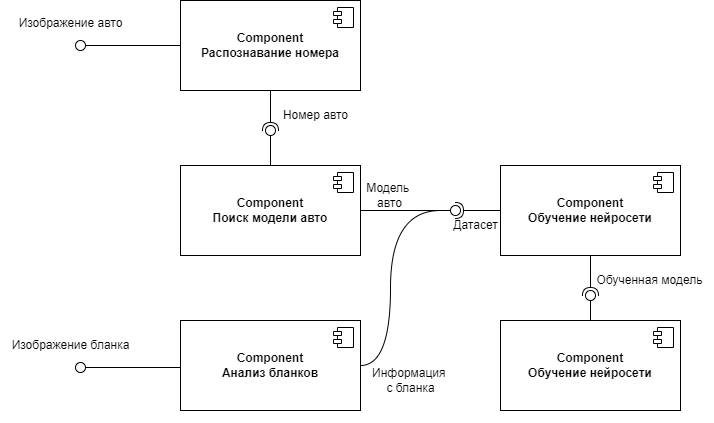
\includegraphics[width=0.8\textwidth]{diag-comp}
    \caption{Диаграмма компонентов}
    \label{f:diag-comp}
\end{figure}

\subsection{Программная реализация модуля для сбора данных}

В данном разделе рассматриваются технологии, используемые при реализации, и описывается сама программная реализация всех компонентов, которые выходят в модуль сбора данных.

\subsubsection{Анализ бланков}

В коде компонента используются библиотеки «cv2» (OpenCV) для обработки изображений, «numpy» для работы с массивами, «argparse» для обработки аргументов командной строки, «imutils» для удобных функций обработки изображений, «csv» для записи результатов в CSV-файл и «pytesseract» для распознавания текста на изображении.
Сам компонент имеет следующие основные функции:

\begin{enumerate}
    \item process\_exam(image\_path). Функция принимает путь к изображению листа. Используя библиотеку «cv2», выполняет следующие шаги обработки изображения:
        \begin{enumerate}
            \item преобразует изображение в оттенки серого, размывает его и применяет пороговое преобразование для выделения контуров;
            \item находит контуры на изображении и выбирает наибольший контур, который предположительно является контуром экзаменационного листа;
            \item используя функцию «four\_point\_transform» из «imutils», выполняет перспективное преобразование изображения, чтобы получить прямоугольный экзаменационный лист;
            \item применяет пороговое преобразование к преобразованному изображению и находит контуры вопросов на экзаменационном листе;
            \item для каждого вопроса находит наибольший контур, который предположительно является контуром выбранного ответа;
            \item определяет выбранные ответы и возвращает результаты в виде списка;
        \end{enumerate}
    \item get\_age(image\_path). Функция принимает путь к изображению документа, содержащего возраст. Используя библиотеку «cv2», выполняет следующие шаги обработки изображения:
        \begin{enumerate}
            \item находит контуры на изображении и выбирает наибольший контур, который предположительно является контуром документа;
            \item используя функцию «four\_point\_transform» из «imutils», выполняет перспективное преобразование изображения, чтобы получить прямоугольный документ;
            \item применяет пороговое преобразование к преобразованному изображению и находит контуры чисел на документе;
            \item используя библиотеку «pytesseract», выполняет распознавание текста на изображении и находит числа, представляющие возраст;
            \item возвращает возраст в виде строки;
        \end{enumerate}
    \item write\_to\_csv(filename, results):
        \begin{enumerate}
            \item функция принимает путь к CSV-файлу и результаты обработки;
            \item используя библиотеку «csv», открывает файл в режиме добавления и записывает результаты в виде строки в CSV-файл;
        \end{enumerate}
    \item blank(path\_in, path\_out, model):
        \begin{enumerate}
            \item функция принимает путь к входному изображению, путь к выходному CSV-файлу и модель (номер экзаменационного листа);
            \item вызывает функции «process\_exam» и «get\_age» для обработки изображения и определения возраста;
            \item добавляет модель и возраст в начало списка результатов;
            \item вызывает функцию «write\_to\_csv» для записи результатов в CSV-файл;
        \end{enumerate}
    \item main():
        \begin{enumerate}
            \item основная функция, которая принимает путь к входному изображению и путь к выходному CSV-файлу с помощью аргументов командной строки;
            \item вызывает функции «process\_exam» и «get\_age» для обработки изображения и определения возраста;
            \item вызывает функцию «write\_to\_csv» для записи результатов в CSV-файл;
        \end{enumerate}
\end{enumerate}

\subsubsection{Поиск модели авто}

При программной реализации данного компонента использовалась библиотеку Selenium для автоматизации веб-браузера. Она включает в себя следующие функции и шаги:
\begin{enumerate}
    \item импортируются необходимые модули: selenium, time, и другие модули, необходимые для работы с Selenium;
    \item указывается путь к драйверу браузера (chromedriver.exe) в переменной «driver\_path»;
    \item указывается URL-адрес веб-сайта, на котором будет выполняться поиск, в переменной «website\_url»;
    \item указывается номер, который будет использоваться в качестве вводного параметра, в переменной «num»;
    \item создается экземпляр браузера Chrome с использованием указанного драйвера в переменной «driver»;
    \item ­определяется функция «site», которая принимает в качестве аргумента номер и выполняет следующие действия:
        \begin{enumerate}
            \item загружается веб-страница с указанным URL-адресом;
            \item на странице вводится номер в поле с именем "identifier";
            \item номер отправляется в поле ввода с помощью метода «send\_keys» и клавиши Enter;
            \item ожидается изменение URL-адреса на веб-странице с использованием «WebDriverWait»;
            \item ожидается 3 секунды для загрузки страницы;
            \item мна странице находится элемент с классом "pit4K", который содержит текст, связанный с номером;
            \item текст из элемента извлекается и разбивается на строки;
            \item результирующий текст объединяется в две строки с помощью «join(lines[:2])»;
            \item возвращается первая строка текста, разделенная запятой и приводится к нижнему регистру;
            \item завершается работа браузера с помощью «driver.quit()»;
        \end{enumerate}
        \item в блоке «if \_\_name\_\_ == "\_\_main\_\_":» вызывается функция «site» с передачей номера в качестве аргумента и выводится результат в консоль.
    \end{enumerate}

\subsubsection{Распознавание номера}

Для работы модуля используются следующие библиотеки и модули:
    \begin{itemize}
        \item PyQt6. Для создания графического интерфейса пользователя и обработки событий;
        \item OpenCV. для обработки изображений и видео, включая разделение видео на кадры и обнаружение номерных знаков;
        \item TensorFlow Lite. Для загрузки и использования моделей машинного обучения для распознавания номеров автомобилей;
        \item NumPy. Для работы с массивами и математических операций;
        \item Matplotlib. Для визуализации результатов обработки изображений;
        \item SciPy. Для преобразования изображений и обнаружения линий;
        \item autoteka и test\_blank. Пользовательские модули для работы с сайтом и создания пустых бланков.
    \end{itemize}

    Функции компонента:
    \begin{enumerate}
        \item load():
            \begin{enumerate}
                \item функция загружает видеофайл из диалогового окна выбора файлов;
                \item использует метод QFileDialog.getOpenFileName() для открытия диалогового окна выбора файлов;
                \item путь к выбранному видеофайлу сохраняется в переменной video\_file в формате Path(video\_file[0]);
            \end{enumerate}
        \item split():
            \begin{enumerate}
                \item функция разделяет видеофайл на отдельные кадры;
                \item создает папку с именем, соответствующим имени исходного видеофайла, если такой папки еще нет;
                \item использует библиотеку moviepy для разделения видео на кадры с заданной частотой кадров (SAVING\_FRAMES\_PER\_SECOND);
                \item каждый кадр сохраняется в папке с именем, соответствующим времени его появления в видео;
            \end{enumerate}
        \item choose():
            \begin{enumerate}
                \item функция распознает номер автомобиля на изображении;
                \item использует модели машинного обучения для обнаружения номерного знака и его распознавания;
                \item производит предварительную обработку изображения, включая изменение размера, преобразование в оттенки серого, применение фильтра Canny для обнаружения границ и преобразование изображения в бинарное;
                \item использует модель TensorFlow Lite для распознавания символов на номерном знаке;
                \item возвращает распознанный номер автомобиля в виде строки;
            \end{enumerate}
        \item recognize():
            \begin{enumerate}
                \item функция вызывается при нажатии на кнопку "Распознать";
                \item вызывает функцию `carplate\_text()` для распознавания номера автомобиля на выбранном изображении;
                \item отображает результат распознавания на метке;
                \item обновляет статистику по количеству распознанных номеров и их вероятности;
                \item проверяет формат распознанного номера и выводит сообщение об ошибке, если формат неверный;
                \item если формат верный, сохраняет результат в массив `arr` и обновляет статистику на метках;
                \item передает полученный номер в компонент определения модели машины;   
            \end{enumerate} 
    \end{enumerate}


\subsection{Программная реализация модуля для обучения нейросети и предсказания интересов}

В данном разделе будет описана программная реализация всех компонентов. Модуль разрабатывался на языке Python в среде разработки Visual Studio Code.

\subsubsection{Обучение нейросети}
Этот скрипт реализует процесс обучения нейронной сети для прогнозирования интересов на основе их возраста и модели авто. При его создании использовались следующие средства:
\begin{itemize}
    \item библиотека pandas. Используется для работы с данными в формате DataFrame, включая загрузку данных из CSV-файла и их предварительную обработку;
    \item библиотека numpy. Применяется для работы с числовыми данными и выполнения математических операций, таких как нормализация числовых данных;
    \item библиотека scikit-learn. Используется для разделения данных на обучающий и тестовый наборы, преобразования категориальных переменных в числовые с помощью OneHotEncoding, подбора оптимальных параметров модели с помощью GridSearchCV и других методов машинного обучения;
    \item библиотека TensorFlow. Применяется для создания и обучения нейронных сетей. В данном скрипте используется Keras API для построения и компиляции модели нейронной сети.
\end{itemize}

Теперь более подробно рассмотрим процесс реализации:
\begin{enumerate}
    \item загрузка данных. Из CSV-файла 'datanew.csv' данные загружаются в объект DataFrame библиотеки pandas. Входными параметрами являются поля Model и Age, а поля Sport, book/films, Science, Travel, Cooking, Politics выходными.
    \item предобработка данных. Категориальный столбец "Model" преобразуется в числовые значения с помощью метода OneHotEncoding из библиотеки sklearn. Нормализация числовых данных о возрасте также выполняется для лучшей работы нейронной сети;
    \item разделение данных. Данные разделяются на обучающий и тестовый наборы с использованием функции train\_test\_split из библиотеки sklearn;
    \item определение функции создания модели. Функция create\_model определяет архитектуру нейронной сети с возможностью настройки различных параметров, таких как количество слоев, количество нейронов, функция активации, dropout rate, оптимизатор и т.д.;
    \item создание модели KerasClassifier. Создается модель KerasClassifier, обертка над моделью Keras, для использования с методом кросс-валидации GridSearchCV из библиотеки sklearn;
    \item задание сетки параметров для подбора. Задаются параметры для поиска лучших комбинаций параметров модели с помощью GridSearchCV;
    \item создание объекта GridSearchCV. Создается объект GridSearchCV с указанными параметрами для поиска оптимальных гиперпараметров модели;
    \item определение обратного вызова EarlyStopping. Обратный вызов EarlyStopping определяется для автоматической остановки обучения, если происходит переобучение модели;
    \item подгонка объекта GridSearchCV к данным. Объект GridSearchCV подгоняется к обучающим данным с использованием метода fit, включая обратный вызов EarlyStopping;
    \item вывод лучших параметров. Выводятся лучшие параметры модели, найденные с помощью GridSearchCV;
    \item оценка модели с лучшими параметрами. Лучшая модель из GridSearchCV оценивается на тестовом наборе данных, и выводится точность предсказания.
\end{enumerate}


\subsubsection{Реализация модуля}

При реализации модуля были написаны 2 скрипта. Один для выполнения предсказаний, другой реализует интерфейс. Использовались следующие средства:
\begin{itemize}
    \item PyQt6. PyQt6 является набором библиотек для Python, предоставляющим интерфейс для работы с графическими приложениями на основе Qt, кросс-платформенного фреймворка для разработки приложений с графическим интерфейсом. В модуле с GUI используется PyQt6 для создания оконного приложения и визуализации элементов пользовательского интерфейса, таких как кнопки, поля ввода и таблица;
    \item TensorFlow. TensorFlow в модуле используется для загрузки обученной модели нейронной сети, выполнения предсказаний и обработки данных;
    \item NumPy. В модуле NumPy используется для предобработки данных и работы с массивами;
    \item Pandas. В модуле Pandas используется для загрузки данных из CSV-файла и предварительной обработки данных перед подачей их на вход нейронной сети;
    \item scikit-learn. В модуле scikit-learn используется для предобработки данных и выполнения OneHotEncoding для категориальных переменных. 
\end{itemize}

Рассмотрим первый скрипт более подробно. Ниже представлен его функционал:
\begin{enumerate}
    \item загрузка обученной модели. В начале модуля загружается обученная модель нейронной сети из файла, созданная и сохраненная в этапе обучения;
    \item преобразование новых данных. Функция preprocess\_new\_data принимает новые данные (модель и возраст) и преобразует их в формат, совместимый с обученной моделью. В частности, она преобразует категориальный столбец "Model" в числовые значения с помощью OneHotEncoding и нормализует числовые данные о возрасте;
    \item получение предсказаний. Функция get\_predictions принимает преобразованные данные и использует обученную модель для выполнения предсказаний. Она возвращает вероятности принадлежности к каждой из категорий интересов;
    \item вывод результатов. Функция print\_results выводит результаты предсказаний в консоль для отладки;
    \item главная функция main. Главная функция main принимает модель и возраст, вызывает описанные выше функции для выполнения предсказаний и форматирует результаты для дальнейшего использования. Она возвращает массив вероятностей принадлежности к каждой категории интересов;
    \item тестирование модули. В блоке if \_\_name\_\_ == "\_\_main\_\_": пример вызова функции main с тестовыми данными и вывод результатов предсказаний в консоль для отладки.
\end{enumerate}

Теперь рассмотрим скрипт, который реализует интерфейс:
\begin{enumerate}
    \item определение графического интерфейса. Создается класс MyWindow, который наследуется от QWidget и представляет собой окно приложения. В методе initUI определяется интерфейс окна, включая надписи, поля ввода, таблицу для отображения результатов и кнопку для выполнения предсказаний;
    \item обработка событий. В методе proc происходит обработка события нажатия на кнопку. Данные из полей ввода для модели и возраста извлекаются с помощью метода toPlainText(). Если оба поля не пустые, вызывается функция main(), описанная в предыдущем скрипте, для выполнения предсказаний. Результаты предсказаний отображаются в таблице;
    \item запуск приложения. В блоке if \_\_name\_\_ == '\_\_main\_\_': создается экземпляр приложения QApplication, создается окно MyWindow, показывается на экране и запускается выполнение приложения с помощью sys.exit(app.exec()).
\end{enumerate}


\subsection{Результат}


В ходе выполения проекта была разработана система, которая выполняет поставленную задачу сбора данных и прогнозирования интересов посетителей автостоянки.


Окно для сбора информации представлено на рисунке~\ref{f:window1}. На экране имеются необходимые кнопки дял выполнения заданых функций.

\begin{figure}[h!]
	\centering
	\vspace{\toppaddingoffigure}
	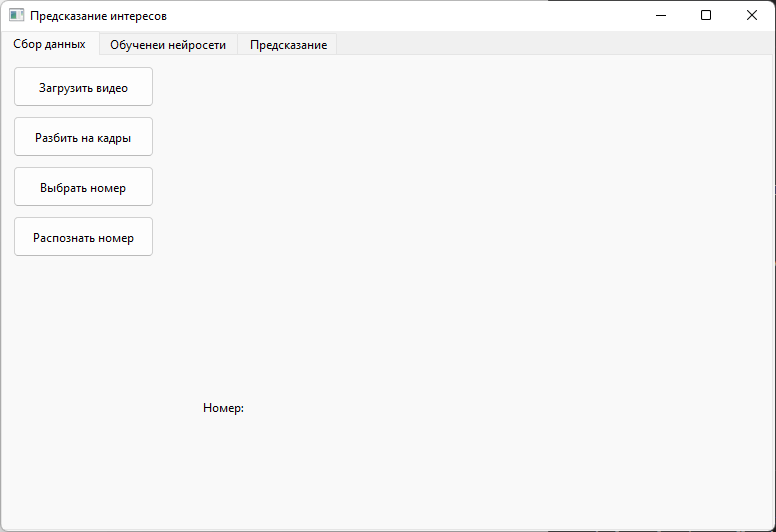
\includegraphics[width=0.5\textwidth]{window1}
	\caption{Окно программы}
	\label{f:window1}
\end{figure}

Выбор изображения представлен на рисунке~\ref{f:choose-pic}. Рядом с кнопками есть место для отрисовкм выбранного изображения.

\begin{figure}[h!]
	\centering
	\vspace{\toppaddingoffigure}
	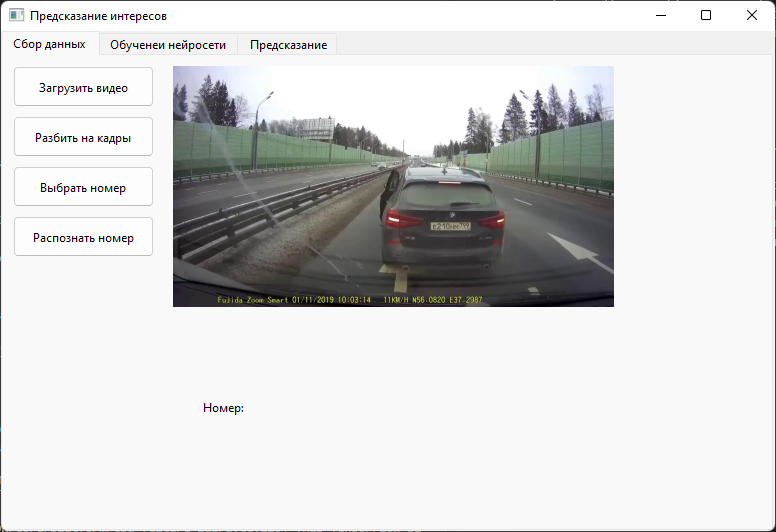
\includegraphics[width=0.5\textwidth]{choose-pic}
	\caption{Выбор изображения}
	\label{f:choose-pic}
\end{figure}

Распознавание номера представлено на рисунке~\ref{f:recognize}.

\begin{figure}[h!]
	\centering
	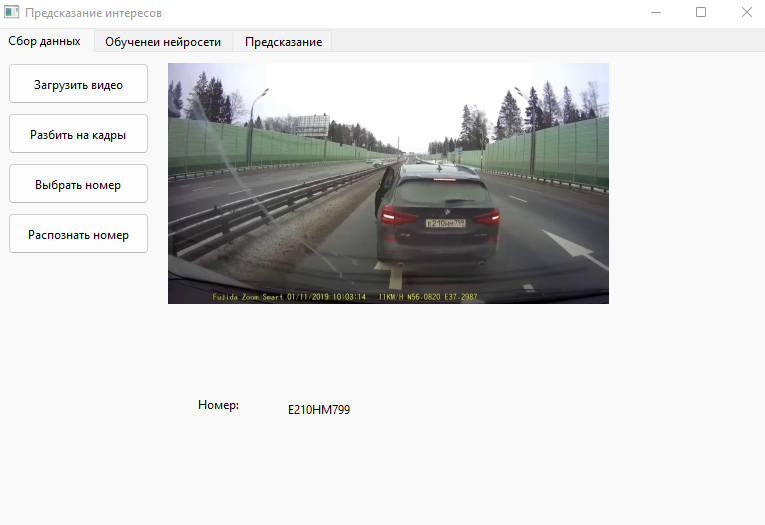
\includegraphics[width=0.5\textwidth]{recognize}
	\caption{Распознавание номера}
	\label{f:recognize}
\end{figure}


\newpage

Дальше происходит переход на сайт для определения модели автомобиля по распознанному номеру (рисунок~\ref{f:ident-model}).

\begin{figure}[h!]
	\centering
    \vspace{\toppaddingoffigure}
	
\includegraphics[width=0.5\textwidth]{ident-model}
	\caption{Определение модели авто}
	\label{f:ident-model}
\end{figure}


После этого предлагается выбрать изображение с бланком (рисунок~\ref{f:blank-examp}).

\begin{figure}[h!]
	\centering
	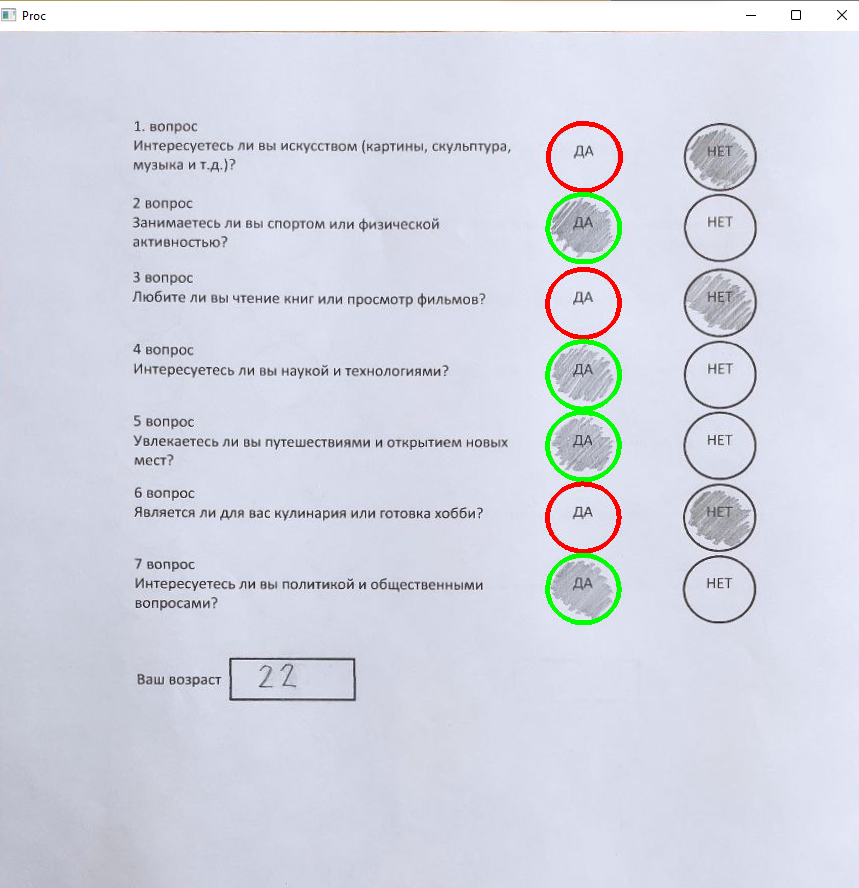
\includegraphics[width=0.5\textwidth]{blank-examp}
	\caption{Бланк опроса}
	\label{f:blank-examp}
\end{figure}


На бланке происходит обводка ответов. красным обводится в случае ответа НЕТ, а зеленым – в случае ответа ДА. Так же происходит считывание возраста, указанного в специальном поле.

Для удобства отладки происходит вывод в консоль (рисунок~\ref{f:console-log}).

\begin{figure}[h]
	\centering
	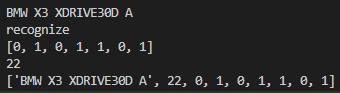
\includegraphics[width=0.5\textwidth]{console-log}
	\caption{Работа программы}
	\label{f:console-log}
\end{figure}

\newpage
Как можно увидеть по рисунку~\ref{f:console-log}, была определена модель автомобиля, так же выведен массив, содержащий ответы на вопросы. «0» означает ответ НЕТ, а «1» - ответ ДА. Кроме того, можно увидеть распознанный возраст «22». В конце все данные объединяются в единое целое, для записи в датасет – файл формата CSV. Результат записи представлен на рисунке~\ref{f:dataset}.

\begin{figure}[h!]
	\centering
    \vspace{\toppaddingoffigure}
	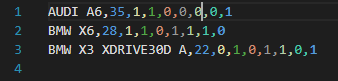
\includegraphics[width=0.5\textwidth]{dataset}
	\caption{Датасет}
	\label{f:dataset}
\end{figure}

\newpage
Окно для обучения нейросети представлено на рисунке~\ref{f:window2}. Имеются 2 кнопки дял выбора файла и начала обучения.

\begin{figure}[h!]
	\centering
    \vspace{\toppaddingoffigure}
	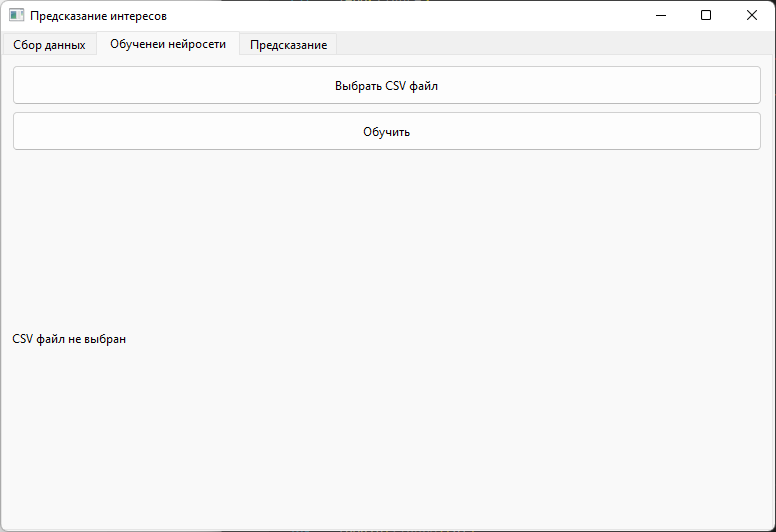
\includegraphics[width=0.5\textwidth]{window2}
	\caption{Окно программы}
	\label{f:window2}
\end{figure}

После выбора файла датасета выводится сообщение о выбранном файле (рисунок~\ref{f:window2.1}). Дальше можно приступать к обучению. По итогу обучения создается модель с расиширением ".keras".

\begin{figure}[h!]
	\centering
    \vspace{\toppaddingoffigure}
	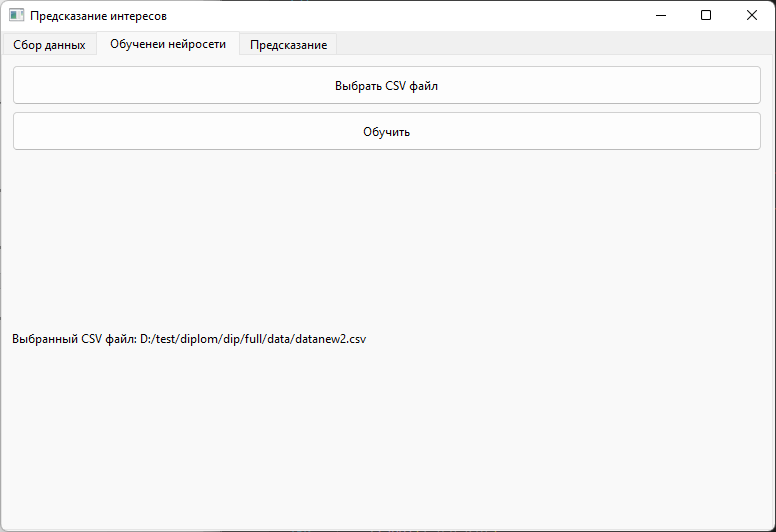
\includegraphics[width=0.5\textwidth]{window2.1}
	\caption{Окно программы}
	\label{f:window2.1}
\end{figure}

\newpage
Окно для предсказания интересов придставелно на рисунке~\ref{f:window3}.
\begin{figure}[h!]
	\centering
    \vspace{\toppaddingoffigure}
	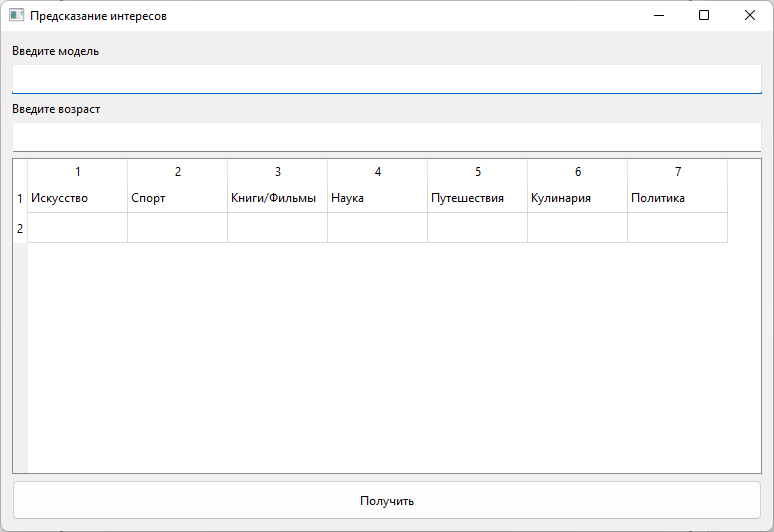
\includegraphics[width=0.5\textwidth]{window3}
	\caption{Окно программы}
	\label{f:window3}
\end{figure}

В поля для ввода необходимо ввести данные: название автомобиля и возраст владельца. После этого нажать на кнопку внизу экрана. Дальше модуль проведет работу, используя обученную модель для прогнозирования интересов. Результат работы представлен на рисунке~\ref{f:res-mod-pred}.
\begin{figure}[h!]
	\centering
    \vspace{\toppaddingoffigure}
	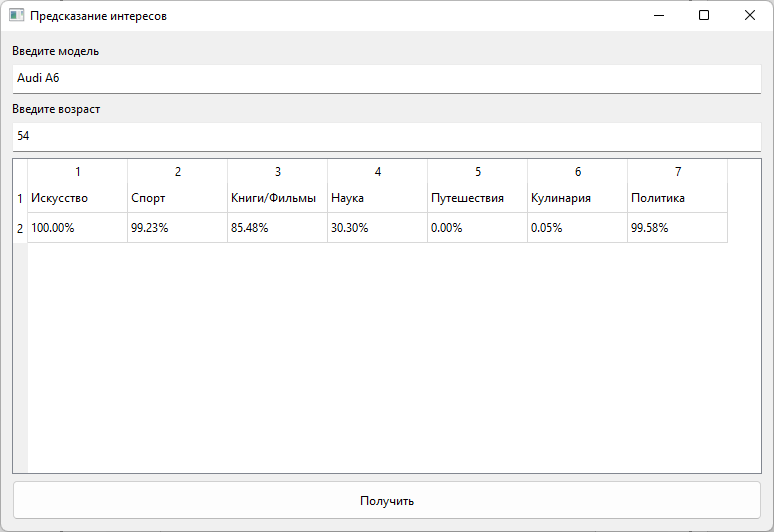
\includegraphics[width=0.5\textwidth]{res-mod-pred}
	\caption{Результат работы модуля}
	\label{f:res-mod-pred}
\end{figure}




\newpage
\section*{Выводы}
В двнном разделе были описаны основные технологии, которые использовались при разработке модулей, из которых состоит система. Было дано пояснение к основным функциям, а также расписан порядок их выполнения.
\newpage

\csection{Заключение}

В ходе выполнения проекта был разработан программная система, которая позволяет собирать информацию об интересах посетителей парковки и прогнозировать эти интересы. Для этого было использовано машинное обучение, методы компьютерного зрения и обработки опросных данных. 

Основной целью проекта было создать систему, которая поможет маркетологам анализировать интересы клиентов.

В процессе работы был проведен анализ предметной области, выявлены актуальность темы и ключевые требования. Были рассмотрены методы анализа данных, машинного обученияя и принцыпы копьютерного зрения.

Для реализации функционала были разработаны следующие компоненты: анализатор бланков, поиск модели автомобиля и распознавание номера. Кроме того были созданы скрипты для обучения нейронной сети с автоматизированным подбором гиперпараметров, а также для работы с обученной моделью. С помощью библиотеки-тюнера были подобраны наилучшие параметры для обучения и выбора оптимальной структуры нейронной сети.

Анализатор бланков позволяет автоматически обрабатывать изображения анкет, извлекать информацию об ответах на вопросы и возрасте. Для этого используются технологии обработки изображений и распознавания текста.

Компонент поиска модели автомобиля обеспечивает автоматизированный доступ к информации о моделях автомобилей. Для этого используется взаимодействие с сайтом, предоставляющим данные о транспортных средствах.

Компонент распознавания номера автомобиля служит для определения номера на изображении. Для этого используется предобученная модель машинного обучения.

В результате работы была разработана программная система, которая может быть использована в реальных задачах, направленных на анализ интересов посетителей парковок. Разработанная система принесет пользу для маркетологов и 
других людей, котороые работают с клиентами. Она помогает легко собирать и анализировать информацию о том, что нравится посетителям парковки. Это позволяет более точно нацеливать 
рекламные компании и предложения, что, в свою очередь, улучшает впечателния клиентов и делает маркетинг более эффективным.
% \newpage

\docappendix{Библиографический список}

\begin{references}
	\item\label{ref:num-methods} Бахвалов Н.С., Жидков Н.П., Кобельников Г.М.
	Численные методы [Текст] – 4-е изд. – М:. БИНОМ. Лаборатория
	знаний, 2006. – 636 с.: ил.
	\item Безрученко Б.П., Смирнов Д.А.
	Статистическое моделирование по временным рядам [Электронный ресурс]
	Cарат. отд-ние Ин-та радиотехники и электроники РАН.
	– Электрон. дан. – Саратов, 2000. – Режим доступа:
	http://www.masters.donntu.edu.ua/2012/fknt/dorosh/library/article4.pdf,
	свободный. - Загл. с экрана.
	\item Перельмутер А.В. Расчетные модели сооружений и возможность их анализа [Текст] / А.В. Перельмутер, В.И.
	Сливкер. Киев: Сталь, 2002. 600 с.
	\item NeuroShell 2 [Электронный ресурс] – Режим доступа: http://www.neuroproject.ru/aboutproduct.php, свободный. –
	Загл. с экрана.
	\item\label{ref:time-series-analysis} Бокс Дж., Дженкинс Г. Анализ временных рядов.
	Прогноз и управление [Текст]. - М.: Мир, 1974.

	\label{ref:total}
\end{references}

\docappendix{Авторская справка}\label{ax:authornote}
\input{pages/authornote.example.tex}


\docappendix{Листинг кода}\label{ax:code}

\begin{lstlisting}
    # Component for searching car models using the autoteka.ru website 
    from selenium import webdriver
    from selenium.webdriver.common.keys import Keys
    from selenium.webdriver.common.by import By
    from selenium.webdriver.support.ui import WebDriverWait  # Импортируем WebDriverWait
    from selenium.webdriver.support import expected_conditions as EC
    import time

    # Path to driver
    driver_path = 'drv/chromedriver-win64/chromedriver.exe'

    # URL link to the page
    website_url = 'https://autoteka.ru/'

    # Initializing the driver
    chrome_service = webdriver.chrome.service.Service(driver_path)
    driver = webdriver.Chrome(service=chrome_service)

    # Function for parsing
    def site(number):
        input = number
        driver.get(website_url)

        input_field = driver.find_element(By.NAME, 'identifier')
        input_field.send_keys(input)
        input_field.send_keys(Keys.ENTER)

        WebDriverWait(driver, 15).until(EC.url_changes(website_url))

        time.sleep(5)

        text_element = driver.find_element(By.CLASS_NAME, 'pit4K')
        text = text_element.text

        time.sleep(3)

        lines = text.split('\n')
        result = ' '.join(lines[:2])

        driver.quit()

        return result.split(',')[0].strip()
\end{lstlisting}

\begin{lstlisting}
    # Component for analyzing forms
    from imutils.perspective import four_point_transform
    from imutils import contours
    import numpy as np
    import argparse
    import imutils
    import cv2
    import csv
    import re
    import pytesseract
    
    # Define the correct answers for the exam (placeholder)
    ANSWER_KEY = {0: 0, 1: 0, 2: 0, 3: 0, 4: 0, 5: 0, 6: 0}
    
    # Path to Tesseract executable
    pytesseract.pytesseract.tesseract_cmd = r'C:\\Program Files\\Tesseract-OCR\\tesseract.exe'
    
    # Tesseract OCR configuration
    custom_config = r'--oem 3 --psm 6'
    
    def process_exam(image_path):
        # Read the input image
        image = cv2.imread(image_path)
        
        # Convert the image to grayscale
        gray = cv2.cvtColor(image, cv2.COLOR_BGR2GRAY)
        
        # Apply GaussianBlur to reduce noise and detail in the image
        blurred = cv2.GaussianBlur(gray, (5, 5), 0)
        
        # Use Canny edge detector to find edges in the image
        edged = cv2.Canny(blurred, 75, 200)
    
        # Find contours in the edged image
        cnts = cv2.findContours(edged.copy(), cv2.RETR_EXTERNAL, cv2.CHAIN_APPROX_SIMPLE)
        cnts = imutils.grab_contours(cnts)
        docCnt = None
    
        # Ensure at least one contour was found
        if len(cnts) > 0:
            # Sort the contours by area, keeping only the largest one
            cnts = sorted(cnts, key=cv2.contourArea, reverse=True)
            for c in cnts:
                # Approximate the contour
                peri = cv2.arcLength(c, True)
                approx = cv2.approxPolyDP(c, 0.02 * peri, True)
                
                # If the approximated contour has four points, assume it's the paper
                if len(approx) == 4:
                    docCnt = approx
                    break
    
        # Apply a perspective transform to obtain a top-down view of the paper
        paper = four_point_transform(image, docCnt.reshape(4, 2))
        warped = four_point_transform(gray, docCnt.reshape(4, 2))
    
        # Apply a binary threshold to the warped image
        thresh = cv2.threshold(warped, 0, 255, cv2.THRESH_BINARY_INV | cv2.THRESH_OTSU)[1]
    
        # Find contours in the thresholded image
        cnts = cv2.findContours(thresh.copy(), cv2.RETR_EXTERNAL, cv2.CHAIN_APPROX_SIMPLE)
        cnts = imutils.grab_contours(cnts)
        questionCnts = []
    
        # Loop over the contours
        for c in cnts:
            (x, y, w, h) = cv2.boundingRect(c)
            ar = w / float(h)
            
            # Filter the contours to find those that correspond to question bubbles
            if (w >= 50) and (h >= 50) and (ar >= 0.9) and (ar <= 1.1):
                questionCnts.append(c)
    
        # Sort the question contours top-to-bottom
        questionCnts = contours.sort_contours(questionCnts, method="top-to-bottom")[0]
        results = []
    
        # Loop over the question groups
        for (q, i) in enumerate(np.arange(0, len(questionCnts), 2)):
            cnts = contours.sort_contours(questionCnts[i:i + 2])[0]
            bubbled = None
            question_result = 0
    
            # Loop over the sorted contours
            for (j, c) in enumerate(cnts):
                mask = np.zeros(thresh.shape, dtype="uint8")
                cv2.drawContours(mask, [c], -1, 255, -1)
    
                mask = cv2.bitwise_and(thresh, thresh, mask=mask)
                total = cv2.countNonZero(mask)
                if bubbled is None or total > bubbled[0]:
                    bubbled = (total, j)
    
            color = (0, 0, 255)
            k = ANSWER_KEY[q]
    
            if k == bubbled[1]:
                question_result = 1
                color = (0, 255, 0)
    
            cv2.drawContours(paper, [cnts[k]], -1, color, 3)
            results.append(question_result)
    
        print(results)
    
        cv2.imshow("Proc", paper)
        cv2.waitKey(0)
    
        return results
    
    def get_age(image_path):
        # Read the input image
        image = cv2.imread(image_path)
        
        # Convert the image to grayscale
        gray = cv2.cvtColor(image, cv2.COLOR_BGR2GRAY)
        
        # Apply GaussianBlur to reduce noise and detail in the image
        blurred = cv2.GaussianBlur(gray, (5, 5), 0)
        
        # Use Canny edge detector to find edges in the image
        edged = cv2.Canny(blurred, 75, 200)
    
        # Find contours in the edged image
        cnts = cv2.findContours(edged.copy(), cv2.RETR_EXTERNAL, cv2.CHAIN_APPROX_SIMPLE)
        cnts = imutils.grab_contours(cnts)
        docCnt = None
    
        # Ensure at least one contour was found
        if len(cnts) > 0:
            # Sort the contours by area, keeping only the largest one
            cnts = sorted(cnts, key=cv2.contourArea, reverse=True)
            for c in cnts:
                # Approximate the contour
                peri = cv2.arcLength(c, True)
                approx = cv2.approxPolyDP(c, 0.02 * peri, True)
                
                # If the approximated contour has four points, assume it's the paper
                if len(approx) == 4:
                    docCnt = approx
                    break
    
        # Apply a perspective transform to obtain a top-down view of the paper
        paper = four_point_transform(image, docCnt.reshape(4, 2))
    
        # Further process the transformed image to find the age
        gray = cv2.cvtColor(paper, cv2.COLOR_BGR2GRAY)
        blurred = cv2.GaussianBlur(gray, (5, 5), 0)
        edged = cv2.Canny(blurred, 75, 200)
    
        cnts = cv2.findContours(edged.copy(), cv2.RETR_EXTERNAL, cv2.CHAIN_APPROX_SIMPLE)
        cnts = imutils.grab_contours(cnts)
        docCnt = None
    
        if len(cnts) > 0:
            cnts = sorted(cnts, key=cv2.contourArea, reverse=True)
            for c in cnts:
                peri = cv2.arcLength(c, True)
                approx = cv2.approxPolyDP(c, 0.02 * peri, True)
                if len(approx) == 4:
                    docCnt = approx
                    break
    
        paper = four_point_transform(paper, docCnt.reshape(4, 2))
    
        gray = cv2.cvtColor(paper, cv2.COLOR_BGR2GRAY)
        thresh = cv2.threshold(gray, 0, 255, cv2.THRESH_BINARY_INV | cv2.THRESH_OTSU)[1]
        
        # Use OCR to extract text from the thresholded image
        text = pytesseract.image_to_string(thresh, config=custom_config)
        
        # Find all two-digit numbers in the extracted text
        number = re.findall(r'\b\d+\b', text)
        two_digit_numbers = ' '.join(num for num in number if len(num) == 2)
        print(two_digit_numbers)
        return two_digit_numbers
    
    def write_to_csv(filename, results):
        # Append the results to a CSV file
        with open(filename, mode='a', newline='') as file:
            writer = csv.writer(file)
            writer.writerow(results)
    
    def blank(path_in, path_out, model):
        print(path_in)
        print(path_out)
        
        # Process the exam and get the age
        results = process_exam(path_in)
        age = get_age(path_in)
        
        # Insert model and age to the results
        results.insert(0, int(age))
        results.insert(0, model)
        
        print(results)
        write_to_csv(path_out, results)
        print("done")
    
    def main():
        # Set up argument parser
        ap = argparse.ArgumentParser()
        ap.add_argument("-i", "--image", required=True, help="path to the input image")
        ap.add_argument("-o", "--output", required=True, help="path to save the output CSV file")
        args = vars(ap.parse_args())
        
        # Process the exam and get the age
        results = process_exam(args["image"])
        age = get_age(args["image"])
        
        # Insert age to the results
        results.insert(0, int(age))
        print(results)
        
        # Write results to the CSV file
        write_to_csv(args["output"], results)
    
    if __name__ == "__main__":
        main()    
\end{lstlisting}

\begin{lstlisting}
    # Component for working with a trained model
    import numpy as np
    import pandas as pd
    import tensorflow as tf
    from sklearn.preprocessing import OneHotEncoder
    import os

    # Transforming new data
    def preprocess_new_data(new_data, full_data):
        # Convert categorical column "Model" to numeric values ​​using OneHotEncoding
        encoder = OneHotEncoder()
        encoder.fit(full_data[['Model']])
        model_encoded = encoder.transform(new_data[['Model']]).toarray()
        
        # Normalization of numerical data (age)
        age = new_data[['Age']].values
        age_normalized = (age - np.mean(full_data['Age'])) / np.std(full_data['Age'])

        # Merging the transformed data
        X_new = np.concatenate([age_normalized, model_encoded], axis=1)
        
        return X_new

    # Receiving Predictions
    def get_predictions(X_new, model_p):
        predictions = model_p.predict(X_new)
        # binary_predictions = np.round(predictions)
        return predictions

    # Output results
    def print_results(binary_predictions):
        # print("New data:")
        # print(new_data)
        print("\nPredictions:")
        np.set_printoptions(threshold=np.inf)
        print(binary_predictions)

    def main(model, age, model_pred):
        
        # Example of new data for testing
        new_data = pd.DataFrame({'Model': [model], 'Age': [int(age)]})

        # Transforming new data
        X_new = preprocess_new_data(new_data, full_data)

        if not os.path.isfile(model_pred):
            raise FileNotFoundError(f"Файл {model_pred} не найден")

        # Check file extension
        if not model_pred.endswith('.keras'):
            raise ValueError("Неправильный формат файла. Ожидался файл с расширением .keras")

        model_p = tf.keras.models.load_model(model_pred)

        # Getting predictions for just one example
        binary_predictions = get_predictions(X_new, model_p)

        art_prediction = binary_predictions[0][0]
        sport_prediction = binary_predictions[0][1]
        book_films_prediction = binary_predictions[0][2]
        science_prediction = binary_predictions[0][3]
        travel_prediction = binary_predictions[0][4]
        cooking_prediction = binary_predictions[0][5]
        politics_prediction = binary_predictions[0][6]

        # Writing to an array
        predictions_array = [art_prediction, sport_prediction, book_films_prediction, science_prediction, travel_prediction, cooking_prediction, politics_prediction]

        return predictions_array
\end{lstlisting}

\begin{lstlisting}
    # Component for training neural networks
    import pandas as pd
    import numpy as np
    import tensorflow as tf
    from tensorflow import keras
    from sklearn.model_selection import train_test_split, GridSearchCV
    from sklearn.preprocessing import OneHotEncoder
    from scikeras.wrappers import KerasClassifier
    from tensorflow.python.keras.callbacks import EarlyStopping, ModelCheckpoint
    from tqdm.keras import TqdmCallback

    # Load the dataset
    data = pd.read_csv('datanew2.csv')

    # Convert the categorical "Model" column to numerical values using OneHotEncoder
    encoder = OneHotEncoder()
    model_encoded = encoder.fit_transform(data[['Model']]).toarray()

    # Normalize the numerical "Age" column
    age = data[['Age']].values
    age_normalized = (age - np.mean(age)) / np.std(age)

    # Combine the normalized age data and the encoded model data
    X = np.concatenate([age_normalized, model_encoded], axis=1)

    # Extract the target variables (interests)
    y = data[['Art', 'Sport', 'Book/Films', 'Science', 'Travel', 'Cooking', 'Politics']].values

    # Split the data into training and test sets
    X_train, X_test, y_train, y_test = train_test_split(X, y, test_size=0.2, random_state=42)

    # Function to create the model with specified parameters
    def create_model(optimizer='adam', num_hidden_layers=2, num_neurons=20, activation='relu', dropout_rate=0.2, learning_rate=0.001):
        # Input layer
        inputs = tf.keras.Input(shape=(X.shape[1],))
        
        # First hidden layer
        x = tf.keras.layers.Dense(num_neurons, activation=activation)(inputs)
        x = tf.keras.layers.Dropout(dropout_rate)(x)
        
        # Additional hidden layers based on the parameter num_hidden_layers
        for _ in range(num_hidden_layers - 1):
            x = tf.keras.layers.Dense(num_neurons, activation=activation)(x)
            x = tf.keras.layers.Dropout(dropout_rate)(x)
        
        # Output layer with sigmoid activation for multi-label classification
        outputs = tf.keras.layers.Dense(7, activation='sigmoid')(x)
        
        # Create the model
        model = tf.keras.Model(inputs=inputs, outputs=outputs)
        
        # Set the optimizer based on the specified parameter
        if optimizer == 'adam':
            optimizer = tf.keras.optimizers.Adam(learning_rate=learning_rate)
        elif optimizer == 'rmsprop':
            optimizer = tf.keras.optimizers.RMSprop(learning_rate=learning_rate)
        elif optimizer == 'sgd':
            optimizer = tf.keras.optimizers.SGD(learning_rate=learning_rate)
        
        # Compile the model
        model.compile(optimizer=optimizer, loss='binary_crossentropy', metrics=['accuracy'])
        return model

    # Create a KerasClassifier with the create_model function
    model = KerasClassifier(model=create_model, verbose=0, epochs=100)

    # Define the grid of parameters for GridSearchCV
    param_grid = {
        'model__num_hidden_layers': [2, 3, 4, 5],
        'model__num_neurons': [20, 30, 40],
        'model__activation': ['relu', 'tanh'],
        'model__dropout_rate': [0.1, 0.2],
        'model__optimizer': ['adam', 'rmsprop', 'sgd'],
        'model__learning_rate': [0.001, 0.01, 0.1]
    }

    # Create a GridSearchCV object
    grid_search = GridSearchCV(estimator=model, param_grid=param_grid, cv=3, verbose=1, n_jobs=-1)

    # Fit the GridSearchCV object to the training data
    grid_search.fit(X_train, y_train)

    # Print the best parameters found by GridSearchCV
    print("Best: %f using %s" % (grid_search.best_score_, grid_search.best_params_))

    # Get the best parameters and create a model with them
    best_params = grid_search.best_params_
    best_model = create_model(
        optimizer=best_params['model__optimizer'],
        num_hidden_layers=best_params['model__num_hidden_layers'],
        num_neurons=best_params['model__num_neurons'],
        activation=best_params['model__activation'],
        dropout_rate=best_params['model__dropout_rate'],
        learning_rate=best_params['model__learning_rate']
    )

    # Define callbacks for early stopping, model checkpointing, and TQDM progress bar
    early_stopping = EarlyStopping(monitor='val_loss', patience=5, restore_best_weights=True)
    model_checkpoint = ModelCheckpoint('model.keras', save_best_only=True, monitor='val_loss', mode='min')
    tqdm_callback = TqdmCallback(verbose=1)

    # Train the best model with the callbacks
    history = best_model.fit(
        X_train, y_train,
        validation_split=0.2,
        epochs=100,
        callbacks=[early_stopping, model_checkpoint, tqdm_callback],
        verbose=0
    )

    # Evaluate the model on the test set
    loss, accuracy = best_model.evaluate(X_test, y_test)
    print(f'Test Accuracy: {accuracy}')
\end{lstlisting}

\begin{lstlisting}
    # Vehicle Number Plate Recognition Component
    import os
    from datetime import timedelta
    from pathlib import Path
    import matplotlib.pyplot as plt
    import cv2
    import numpy as np
    import re
    import imutils
    import pytesseract
    import pytesseract as tess
    tess.pytesseract.tesseract_cmd = r'Tesseract-OCR\tesseract.exe'
    from PyQt6 import uic
    from PyQt6.QtGui import QPixmap
    from PyQt6.QtWidgets import QApplication, QFileDialog, QMessageBox
    from imutils import contours
    from moviepy.editor import VideoFileClip
    import json
    import sqlite3
    import itertools
    import tensorflow as tf
    from skimage.feature import canny
    from skimage.transform import hough_line, hough_line_peaks, rotate
    from skimage.color import rgb2gray

    import matplotlib.gridspec as gridspec
    import cv2

    import autoteka
    import test_blank

    # Constants for saving frames per second from video
    SAVING_FRAMES_PER_SECOND = 1

    # Load the UI design file
    Form, Window = uic.loadUiType("Parking.ui")

    # Initialize the application and load the UI window
    app = QApplication([])
    window = Window()
    form = Form()
    form.setupUi(window)
    window.show()

    # Global variables to store the paths of video, image, and the result
    video_file = ''
    image_file = ''
    result = ''
    arr = []

    # Function to format the time delta for naming frames
    def format_timedelta(td):
        result = str(td)
        try:
            result, ms = result.split(".")
        except ValueError:
            return result + ".00".replace(":", "-")

        ms = round(int(ms) / 10000)
        return f"{result}.{ms:02}".replace(":", "-")

    # Function to load the video file
    def load():
        global video_file
        video_file = QFileDialog.getOpenFileName()
        path = Path(video_file[0])
        video_file = path.name
        print("load")

    # Function to split the video into frames
    def split():
        video_clip = VideoFileClip(video_file)
        filename, _ = os.path.splitext(video_file)

        if not os.path.isdir(filename):
            os.mkdir(filename)

        saving_frames_per_second = min(video_clip.fps, SAVING_FRAMES_PER_SECOND)
        step = 1 / video_clip.fps if saving_frames_per_second == 0 else 1 / saving_frames_per_second

        for current_duration in np.arange(0, video_clip.duration, step):
            frame_duration_formatted = format_timedelta(timedelta(seconds=current_duration)).replace(":", "-")
            frame_filename = os.path.join(filename, f"frame{frame_duration_formatted}.jpg")

            video_clip.save_frame(frame_filename, current_duration)
        print("split")

    # Function to check the format of the recognized license plate
    def check_format(variable):
        pattern = r'^[A-Z]\d{3}[A-Z]{2}\d{3}$'
        pattern2 = r'^[A-Z]\d{3}[A-Z]{2}\d{2}$'
        if re.match(pattern, variable) or re.match(pattern2, variable):
            return True
        else:
            return False

    # Function to choose an image file for recognition
    def choose():
        global image_file
        image_file = QFileDialog.getOpenFileName()
        image_file = image_file[0]
        form.label_6.setPixmap(QPixmap(image_file))
        form.label_6.setScaledContents(True)
        print("choose")

    # Function to recognize text from the car plate
    def carplate_text():
        global image_file

        image0 = cv2.imread(image_file)
        image_height, image_width, _ = image0.shape
        image = cv2.resize(image0, (1024, 1024))
        image = image.astype(np.float32)
        paths = 'model/recognize/model_resnet.tflite'
        interpreter = tf.lite.Interpreter(model_path=paths)
        interpreter.allocate_tensors()
        input_details = interpreter.get_input_details()
        output_details = interpreter.get_output_details()
        X_data1 = np.float32(image.reshape(1, 1024, 1024, 3))

        interpreter.set_tensor(input_details[0]['index'], X_data1)
        interpreter.invoke()
        detection = interpreter.get_tensor(output_details[0]['index'])
        net_out_value2 = interpreter.get_tensor(output_details[1]['index'])
        net_out_value3 = interpreter.get_tensor(output_details[2]['index'])
        net_out_value4 = interpreter.get_tensor(output_details[3]['index'])

        img = image0
        razmer = img.shape

        img2 = cv2.cvtColor(img, cv2.COLOR_BGR2RGB)
        img3 = img[:, :, :]

        number = 0
        while number < len(detection[0][number]) and detection[0, number, 0] > 0.9:
            number = number + 1

        box_x = int(detection[0, number, 0] * image_height)
        box_y = int(detection[0, number, 1] * image_width)
        box_width = int(detection[0, number, 2] * image_height)
        box_height = int(detection[0, number, 3] * image_width)

        cv2.rectangle(img2, (box_y, box_x), (box_height, box_width), (230, 230, 21), thickness=5)

        net_out_value3

        image = image0[box_x:box_width, box_y:box_height, :]
        img2 = cv2.cvtColor(image, cv2.COLOR_BGR2RGB)

        grayscale = rgb2gray(image)
        edges = canny(grayscale, sigma=3.0)
        out, angles, distances = hough_line(edges)
        h, theta, d = out, angles, distances
        angle_step = 0.5 * np.diff(theta).mean()
        d_step = 0.5 * np.diff(d).mean()
        bounds = [np.rad2deg(theta[0] - angle_step),
                np.rad2deg(theta[-1] + angle_step),
                d[-1] + d_step, d[0] - d_step]

        _, angles_peaks, _ = hough_line_peaks(out, angles, distances, num_peaks=20)
        angle = np.mean(np.rad2deg(angles_peaks))

        if 0 <= angle <= 90:
            rot_angle = angle - 90
        elif -45 <= angle < 0:
            rot_angle = angle - 90
        elif -90 <= angle < -45:
            rot_angle = 90 + angle
        if abs(rot_angle) > 20:
            rot_angle = 0

        rotated = rotate(image, rot_angle, resize=True) * 255
        rotated = rotated

        rotated1 = rotated[:, :, :]
        if rotated.shape[1] / rotated.shape[0] < 2:
            minus = np.abs(int(np.sin(np.radians(rot_angle)) * rotated.shape[0]))
            rotated1 = rotated[minus:-minus, :, :]
            print(minus)

        lab = cv2.cvtColor(rotated1, cv2.COLOR_BGR2LAB)
        l, a, b = cv2.split(lab)
        clahe = cv2.createCLAHE(clipLimit=3.0, tileGridSize=(8, 8))
        cl = clahe.apply(l)
        limg = cv2.merge((cl, a, b))
        final = cv2.cvtColor(limg, cv2.COLOR_LAB2BGR)

        letters = ['0', '1', '2', '3', '4', '5', '6', '7', '8', '9', 'A', 'B', 'C', 'E', 'H', 'K', 'M', 'O', 'P', 'T', 'X',
                'Y']

        def decode_batch(out):
            ret = []
            for j in range(out.shape[0]):
                out_best = list(np.argmax(out[j, 2:], 1))
                out_best = [k for k, g in itertools.groupby(out_best)]
                outstr = ''
                for c in out_best:
                    if c < len(letters):
                        outstr += letters[c]
                ret.append(outstr)
            return ret

        paths = 'model/recognize/model1_nomer.tflite'
        interpreter = tf.lite.Interpreter(model_path=paths)
        interpreter.allocate_tensors()

        input_details = interpreter.get_input_details()
        output_details = interpreter.get_output_details()
        img = final
        img = cv2.cvtColor(img, cv2.COLOR_BGR2GRAY)
        img = cv2.resize(img, (128, 64))
        img = img.astype(np.float32)
        img /= 255

        img1 = img.T
        img1.shape
        X_data1 = np.float32(img1.reshape(1, 128, 64, 1))
        input_index = (interpreter.get_input_details()[0]['index'])
        interpreter.set_tensor(input_details[0]['index'], X_data1)

        interpreter.invoke()

        net_out_value = interpreter.get_tensor(output_details[0]['index'])
        pred_texts = decode_batch(net_out_value)
        pred_texts

        fig = plt.figure(figsize=(10, 10))
        outer = gridspec.GridSpec(2, 1, wspace=10, hspace=0.1)
        ax1 = plt.Subplot(fig, outer[0])
        fig.add_subplot(ax1)
        ax2 = plt.Subplot(fig, outer[1])
        fig.add_subplot(ax2)
        return pred_texts[0]

    # Function to recognize the license plate and display information
    def recognize():
        global result
        result = carplate_text().upper()
        print(result)
        if result == '':
            QMessageBox.information(None, "Ошибка распознания", "НЕ РАСПОЗНАНО")
        elif check_format(result) != True:
            QMessageBox.information(None, "Ошибка формата", "Результат:" + result)
        else:
            form.label_7.setText(result)

            count = 0
            for i in range(len(arr)):
                if arr[i][0] == result:
                    count += 1

            if count == 0:
                arr.append([result, 1])
            else:
                for i in range(len(arr)):
                    if arr[i][0] == result:
                        arr[i][1] += 1

            for i in range(len(arr)):
                if arr[i][0] == result:
                    form.label_2.setText(str(arr[i][1]))
                    if arr[i][1] < 5:
                        form.label_5.setText('0%')
                    elif 5 <= arr[i][1] < 10:
                        form.label_5.setText('5%')
                    elif 10 <= arr[i][1] < 20:
                        form.label_5.setText('10%')
                    else:
                        form.label_5.setText('15%')
        
        model = autoteka.site(result)
        print(model)
        print("recognize")

        file_path, _ = QFileDialog.getOpenFileName()
        test_blank.blank(file_path, 'data/data.csv', model)

    # Connect UI buttons to their respective functions
    form.pushButton.clicked.connect(load)
    form.pushButton_2.clicked.connect(split)
    form.pushButton_3.clicked.connect(choose)
    form.pushButton_4.clicked.connect(recognize)

    # Start the application event loop
    app.exec()
\end{lstlisting}

\begin{lstlisting}
    #Interface
    # Importing necessary modules and libraries
    from PyQt6.QtWidgets import (
        QApplication, 
        QWidget, 
        QPushButton, 
        QLabel, 
        QVBoxLayout, 
        QTextEdit, 
        QTableWidget, 
        QTableWidgetItem,
        QTabWidget,
        QMainWindow,
        QFileDialog,
        QMessageBox
    )
    from PyQt6 import QtCore

    # Constant for saving frames per second from a video
    SAVING_FRAMES_PER_SECOND = 1

    # List of interest categories
    list_int = ["Искусство", "Спорт", "Книги/Фильмы", "Наука", "Путешествия", "Кулинария", "Политика"]

    # Global variables for storing file paths and results
    video_file = ''
    image_file = ''
    result = ''
    arr = []

    # Main window class inheriting from QMainWindow
    class MainWindow(QMainWindow):
        def __init__(self):
            super().__init__()

            self.setWindowTitle("Предсказание интересов")
            self.setGeometry(400, 250, 750, 500)

            # Creating a tab widget and setting it as the central widget
            self.tabs = QTabWidget()
            self.setCentralWidget(self.tabs)

            # Creating tabs
            self.create_tabs()

            self.model_pred = ""

        # Method to create tabs
        def create_tabs(self):
            # Creating the first tab for data collection
            tab1 = QWidget()
            
            self.pushButton = QPushButton(tab1)
            self.pushButton.setGeometry(QtCore.QRect(10, 10, 141, 41))
            self.pushButton.setObjectName("pushButton")
            self.pushButton.clicked.connect(self.load)
            self.pushButton.setText("Загрузить видео")

            self.pushButton_2 = QPushButton(tab1)
            self.pushButton_2.setGeometry(QtCore.QRect(10, 60, 141, 41))
            self.pushButton_2.setObjectName("pushButton_2")
            self.pushButton_2.clicked.connect(self.split)
            self.pushButton_2.setText("Разбить на кадры")

            self.pushButton_3 = QPushButton(tab1)
            self.pushButton_3.setGeometry(QtCore.QRect(10, 110, 141, 41))
            self.pushButton_3.setObjectName("pushButton_3")
            self.pushButton_3.clicked.connect(self.choose)
            self.pushButton_3.setText("Выбрать номер")

            self.pushButton_4 = QPushButton(tab1)
            self.pushButton_4.setGeometry(QtCore.QRect(10, 160, 141, 41))
            self.pushButton_4.setObjectName("pushButton_4")
            self.pushButton_4.clicked.connect(self.recognize)
            self.pushButton_4.setText("Распознать номер")

            self.label_6 = QLabel(tab1)
            self.label_6.setGeometry(QtCore.QRect(170, 10, 441, 241))
            self.label_6.setText("")
            self.label_6.setAlignment(QtCore.Qt.AlignmentFlag.AlignCenter)
            self.label_6.setObjectName("label_6")

            self.label_3 = QLabel(tab1)
            self.label_3.setGeometry(QtCore.QRect(200, 340, 71, 21))
            self.label_3.setText("Номер:")
            self.label_3.setObjectName("label_3")

            self.label_7 = QLabel(tab1)
            self.label_7.setGeometry(QtCore.QRect(290, 340, 161, 31))
            self.label_7.setText("")
            self.label_7.setObjectName("label_7")

            # Creating the second tab for neural network training
            tab2 = QWidget()
            tab2_layout = QVBoxLayout()

            self.pushButton_csv = QPushButton(tab2)
            self.pushButton_csv.setText("Выбрать CSV файл")
            self.pushButton_csv.setFixedSize(750, 40)
            self.pushButton_csv.clicked.connect(self.choose_csv_file)
            tab2_layout.addWidget(self.pushButton_csv)

            self.pushButton_learn = QPushButton(tab2)
            self.pushButton_learn.setText("Обучить")
            self.pushButton_learn.setFixedSize(750, 40)
            self.pushButton_learn.clicked.connect(self.learn)
            tab2_layout.addWidget(self.pushButton_learn)

            self.label_csv = QLabel(tab2)
            self.label_csv.setText("CSV файл не выбран")
            tab2_layout.addWidget(self.label_csv)

            tab2.setLayout(tab2_layout)

            # Creating the third tab for prediction
            tab3 = QWidget()
            tab3_layout = QVBoxLayout()

            self.label_model = QLabel('Введите модель', tab3)
            self.label_age = QLabel('Введите возраст', tab3)

            self.text_edit_model = QTextEdit(tab3)
            self.text_edit_model.setFixedSize(750, 30)
            
            self.text_edit_age = QTextEdit(tab3)
            self.text_edit_age.setFixedSize(750, 30)

            self.table = QTableWidget(tab3)
            self.table.setColumnCount(7)
            self.table.setRowCount(2)

            for col in range(7):
                item = QTableWidgetItem(list_int[col])
                self.table.setItem(0, col, item)

            self.button_predict = QPushButton('Получить', tab3)
            self.button_predict.setFixedSize(750, 40)
            self.button_predict.clicked.connect(self.proc)

            self.button_choose_file = QPushButton('Выбрать файл модели', tab3)
            self.button_choose_file.setFixedSize(750, 40)
            self.button_choose_file.clicked.connect(self.choose_model_file)

            # Adding widgets to the third tab
            tab3_layout.addWidget(self.label_model)
            tab3_layout.addWidget(self.text_edit_model)
            tab3_layout.addWidget(self.label_age)
            tab3_layout.addWidget(self.text_edit_age)
            tab3_layout.addWidget(self.button_choose_file)
            tab3_layout.addWidget(self.table)
            tab3_layout.addWidget(self.button_predict)

            tab3.setLayout(tab3_layout)

            # Adding tabs to the QTabWidget
            self.tabs.addTab(tab1, "Сбор данных")
            self.tabs.addTab(tab2, "Обучение нейросети")
            self.tabs.addTab(tab3, "Предсказание")

        # Placeholder method for learning
        def learn(path):
            pass

        # Method to choose a CSV file
        def choose_csv_file(self):
            file_dialog = QFileDialog()
            options = file_dialog.options()
            file_name, _ = QFileDialog.getOpenFileName(self, "Выберите CSV файл", "", "CSV Files (*.csv);;All Files (*)", options=options)
            if file_name:
                self.csv_file = file_name
                self.label_csv.setText(f"Выбранный CSV файл: {file_name}")
            print(self.csv_file)

        # Method to choose a model file
        def choose_model_file(self):
            file_dialog = QFileDialog()
            options = file_dialog.options()
            file_name, _ = QFileDialog.getOpenFileName(self, "Выберите файл модели", "", "Model Files (*.keras);;All Files (*)", options=options)
            if file_name:
                self.model_pred = file_name 
            print(self.model_pred)
            
        # Method to process the model and age input and get predictions
        def proc(self):
            model = self.text_edit_model.toPlainText()
            age = self.text_edit_age.toPlainText()
            if (model != "") & (age != "") & (self.model_pred != ""):
                predictions = test_single.main(model, age, self.model_pred)
                print(predictions)
                for col in range(7):
                    predictions[col] = float(predictions[col])
                    item = QTableWidgetItem(str("{:2.2f}".format(predictions[col] * 100)) + "%")
                    self.table.setItem(1, col, item)

    if __name__ == "__main__":
        app = QApplication(sys.argv)
                
        window = MainWindow()
        window.show()
                
        sys.exit(app.exec()) 
\end{lstlisting}


\docappendix[Справочное]{Библиографический список}

\begin{references}
	\item\label{ref:data-collection} Data Collection [Электронный ресурс] – Режим доступа: https://www.tutorialspoint.com/data-collection, свободный. – Загл. с экрана.

	\item\label{ref:data-analysis} Анализ данных [Электронный ресурс] – Режим доступа: https://en.wikipedia.org/wiki/Data\_analysis, свободный. – Загл. с экрана.

	\item\label{ref:data-visualization} Визуализация данных [Электронный ресурс] – Режим доступа: https://practicum.yandex.ru/blog/vizualizaciya-dannyh/, свободный. – Загл. с экрана.

	\item\label{ref:machine-learning} Машинное обучение: методы и способы [Электронный ресурс] – Режим доступа: https://www.osp.ru/cio/2018/05/13054535, свободный. – Загл. с экрана.

	\item\label{ref:marketing} Медведев П.М. Организация маркетинговой службы с нуля [Текст] ЗАО Издательский дом «Питер». 2005. – 224 с.: ил.

	\item\label{ref:res-net} Exploring ResNet50: An In-Depth Look at the Model Architecture and Code Implementation [Электронный ресурс] – Режим доступа: https://medium.com/@nitishkundu1993/exploring-resnet50-an-in-depth-look-at-the-model-architecture-and-code-implementation-d8d8fa67e46f, свободный. – Загл. с экрана.

	\item\label{ref:cnn-lstm} CNN-LSTM Architecture and Image Captioning [Электронный ресурс] – Режим доступа: https://medium.com/analytics-vidhya/cnn-lstm-architecture-and-image-captioning-2351fc18e8d7, свободный. – Загл. с экрана.
	
	\item\label{ref:neuron} Дюк В.А., Флегонтов А.В., Фомина И.К. Применение технологий интеллектуального анализа данных в естественнонаучных, технических и гуманитарных областях [Текст] Известия Российского государственного педагогического университета им. А.И. Герцена. 2011. No 138.

	\item\label{ref:back-error} Метод обратного распространения ошибки [Электронный ресурс] – Режим доступа: https://education.yandex.ru/handbook/ml/article/metod-obratnogo-rasprostraneniya-oshibki, свободный. – Загл. с экрана.

	\item\label{ref:neuron-model} Neurons in Neural Networks [Электронный ресурс] – Режим доступа: https://www.baeldung.com/cs/neural-networks-neurons, свободный. – Загл. с экрана.

	\item\label{ref:nbc} Наивный байесовский классификатор [Электронный ресурс] – Режим доступа: https://ru.wikipedia.org/wiki/Наивный\_байесовский\_классификатор, свободный. – Загл. с экрана.

	\item\label{ref:log-reg} Пампел Фред, Цвиркун Дмитрий, Груздев Артем. Логистическая регрессия [Текст] ДМК-Пресс, 2023 г. – 218 с.: ил.

	
	\label{ref:total}
\end{references}



} {
	% Привер файла содержимого документа
% Измените подключаемые файлы в зависимости от вашей структуры документа


\csection{Введение}

В современном мире сбор и анализ данных играют ключевую роль в принятии решений во многих сферах деятельности. 
Благодаря развитию технологий, стало возможным эффективно использовать огромные объемы данных для улучшения 
различных процессов и повышения эффективности работы. В особенности, методы компьютерного зрения и искусственного 
интеллекта открывают новые возможности для автоматизации и оптимизации задач, которые ранее выполнялись вручную.

С развитием технологий обработки данных и машинного обучения, особенно нейронных сетей, стало возможным решать 
сложные задачи, такие как распознавание образов, анализ поведения, предсказания исходов каких-любо событи и так далее. 
Эти технологии находят широкое применение в самых разных областях, от маркетинга и розничной 
торговли до здравоохранения и транспорта.

Современные маркетологи сталкиваются с необходимостью глубоко понимать интересы и предпочтения своих клиентов, чтобы создавать эффективные стратегии и кампании. Проект по автоматизации процесса сбора и анализа интересов клиентов автостоянки предоставляет маркетологам мощный инструмент для достижения этой цели.

Благодаря полученным данным, маркетологи смогут более точно сегментировать аудиторию, разрабатывать персонализированные предложения и эффективно проводить рекламные кампании. Это приведет к улучшению взаимодействия с клиентами, увеличению их лояльности и, в конечном итоге, к росту продаж и прибыли компании.

Исходя из выше сказанного, было принято решение о создании системы, которая смогла бы автоматизировать процесс сбора и 
анализа интересов клиентов автостоянки, для того чтобы предоставить пользователям информацию о посетителях.

\pagebreak


\section{Анализ предметной области}

\subsection{Машина времени}

Машина времени является гипотетическим устройством, способным перемещаться во времени, обеспечивая возможность путешествия в прошлое или будущее. В связи с этим, анализ предметной области машины времени включает следующие аспекты:


\begin{enumerate}
	\item физические принципы: необходимо изучить теоретические основы, согласно которым могла бы функционировать машина времени. Это может включать обсуждение специальной теории относительности, черных дыр, петель времени и других концепций из физики;

	\item технические особенности: рассмотрим возможные способы построения и дизайна машины времени. Какие технологии или материалы могут быть использованы для ее создания? Какие опасности или препятствия могут возникнуть при ее конструировании?

	\item парадоксы времени: проанализируем различные парадоксы, которые могут возникнуть при использовании машины времени, такие как "парадокс дедушки" или "парадокс самовыполнения". Какие последствия они могут иметь для временных путешественников?

	\item этические и социальные аспекты: обсудим влияние машины времени на общество и индивидуума. Какие этические вопросы возникают при использовании данной технологии? Какие последствия она может иметь для личной и мировой истории?

	\item возможные приложения: рассмотрим потенциальные области применения машины времени, такие как исследования истории, изменение прошлого или будущего, предсказание событий и т. д.
\end{enumerate}

\subsection{Сравнение аналогов}

Машина времени 1:
\begin{itemize}
	\item перемещает человека в прошлое или будущее;
	\item имеет ограничение по количеству путешествий во времени;
	\item не поддерживает контроль точного места приземления.
\end{itemize}

Машина времени 2:
\begin{itemize}
	\item позволяет путешествовать во времени как в прошлое, так и в будущее;
	\item имеет более сложную систему навигации и управления;
	\item предоставляет дополнительные возможности и функции.
\end{itemize}

Машина времени 3:
\begin{itemize}
	\item позволяет точно указывать дату, время и место для путешествия;
	\item обладает самой передовой технологией и функционалом;
	\item эффективнее и безопаснее других машин времени.
\end{itemize}

Эти машины времени можно сравнивать через их уникальные особенности, функционал, надежность и возможности путешествия. Каждая из них обладает своими преимуществами и ограничениями, что делает их различными в использовани

В таблице \ref{t:comp-an} представлено сравнение аналагов.

\begin{table}[ht]

	\centering
	\Large
	\begin{threeparttable}
		\caption{Сравнение аналогов}
		\label{t:comp-an}
		\begin{tabularx}{\textwidth}{|X|c|c|c|}
			\hline
			Критерии \textbackslash\ Аналоги & Машина времени 1 & Машина времени 2 & Машина времени 3 \\
			\hline
			Критерий 1
			                                 & нет              & да               & да               \\
			\hline
			Критерий 2
			                                 & нет              & да               & да               \\
			\hline
			Критерий 3
			                                 & да               & да               & нет              \\
			\hline
			Критерий 4
			                                 & нет              & нет              & да               \\
			\hline
		\end{tabularx}
	\end{threeparttable}
	\vspace{\bottompaddingoftable}
\end{table}

Таким образом разработка машины времени является актуальной.

\section*{Выводы}


Анализ предметной области машины времени требует не только фантазии и творческого мышления, но и глубоких знаний в области физики, философии, этики и технологии.



\newpage

\section{Структура машины времени}

Структура машины времени представлена на рисунке~\ref{f:time-machine}.


\begin{figure}[ht]
	\centering
	\vspace{\toppaddingoffigure}
	
\includegraphics[width=0.7\textwidth]{time-machine}
	\caption{Структура машины времени}
	\label{f:time-machine}
\end{figure}


Разработка структуры машины времени является сложной задачей, поскольку такое устройство находится за пределами существующих научных и инженерных возможностей. Однако, если мы предположим, что машина времени возможна, то ее структура, вероятно, будет иметь следующие основные компоненты:

\begin{enumerate}
	\item часовой механизм: стандартный механизм, который управляет передвижением во времени, аналогично тому, как часовой механизм контролирует передвижение стрелок на циферблате часов;

	\item энергетический источник: мощный источник энергии, способный обеспечить работу машины времени и перемещение объектов во времени;

	\item контрольная система: комплекс алгоритмов и программного обеспечения, которые контролируют точное время и координируют перемещение во времени;

	\item защитные механизмы: системы, предотвращающие нежелательное перемещение во времени или обеспечивающие безопасность при использовании машины времени;

	\item интерфейс пользователя: устройства ввода и вывода, позволяющие пользователю программировать желаемые временные точки или координировать перемещение во времени;

	\item материалы и конструкция: специальные материалы и компоненты, обеспечивающие устойчивость и работоспособность машины времени.
\end{enumerate}

Хотя это очень упрощенное описание возможной структуры машины времени, это может помочь представить основные компоненты, которые потребуются для того, чтобы создать такое устройство. Однако необходимо помнить, что вышеописанная концепция является вымышленной и не имеет научного обоснования.


Пример ссылки на источник \refref{ref:num-methods}.

Пример еще ссылки на источник \refref{ref:time-series-analysis}.

Код представлен в приложении \ref{ax:code}.

Авторская справка представлена в приложении \ref{ax:authornote}.

Какое-то справочное приложение представлено в приложении \ref{ax:ref}.


\subsection{Расчёты}

Расчёты представлены ниже

\begin{gather}
	a = \tan(\frac{\alpha}{2})*a*\pi, \\
	\bigtriangleup b = \cos(\beta)*a, \\
	c = \sin{\beta}.
\end{gather}


\examplecommand

\newpage

\section{Программная реализация}
В данном разделе будут рассмотрены средства, методы и библиотеки, которые использовались при программной реализации. Кроме того, тут будут описаны основные функции, которые реализованы в модулях, и то как они работают. Так же будет рассмотрен процесс работы системы на заданном примере. 

Для наглядного описания взаимодействия разработанных компонентов ниже приведена диаграмма вариантов использования (рисунок~\ref{f:diag-comp}).

\begin{figure}[h!]
    \centering
    \vspace{\toppaddingoffigure}
    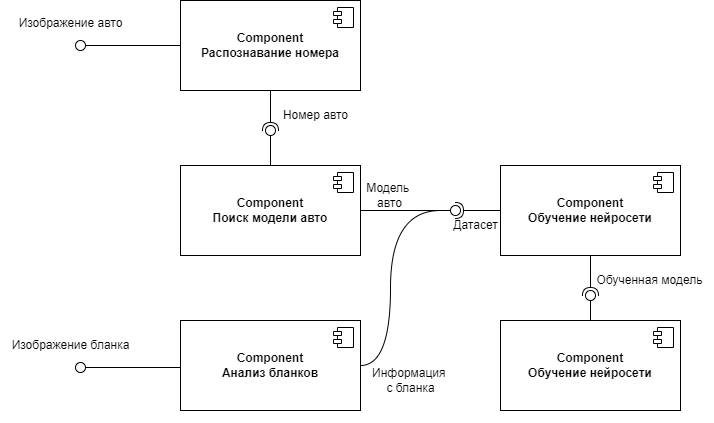
\includegraphics[width=0.8\textwidth]{diag-comp}
    \caption{Диаграмма компонентов}
    \label{f:diag-comp}
\end{figure}

\subsection{Программная реализация модуля для сбора данных}

В данном разделе рассматриваются технологии, используемые при реализации, и описывается сама программная реализация всех компонентов, которые выходят в модуль сбора данных.

\subsubsection{Анализ бланков}

В коде компонента используются библиотеки «cv2» (OpenCV) для обработки изображений, «numpy» для работы с массивами, «argparse» для обработки аргументов командной строки, «imutils» для удобных функций обработки изображений, «csv» для записи результатов в CSV-файл и «pytesseract» для распознавания текста на изображении.
Сам компонент имеет следующие основные функции:

\begin{enumerate}
    \item process\_exam(image\_path). Функция принимает путь к изображению листа. Используя библиотеку «cv2», выполняет следующие шаги обработки изображения:
        \begin{enumerate}
            \item преобразует изображение в оттенки серого, размывает его и применяет пороговое преобразование для выделения контуров;
            \item находит контуры на изображении и выбирает наибольший контур, который предположительно является контуром экзаменационного листа;
            \item используя функцию «four\_point\_transform» из «imutils», выполняет перспективное преобразование изображения, чтобы получить прямоугольный экзаменационный лист;
            \item применяет пороговое преобразование к преобразованному изображению и находит контуры вопросов на экзаменационном листе;
            \item для каждого вопроса находит наибольший контур, который предположительно является контуром выбранного ответа;
            \item определяет выбранные ответы и возвращает результаты в виде списка;
        \end{enumerate}
    \item get\_age(image\_path). Функция принимает путь к изображению документа, содержащего возраст. Используя библиотеку «cv2», выполняет следующие шаги обработки изображения:
        \begin{enumerate}
            \item находит контуры на изображении и выбирает наибольший контур, который предположительно является контуром документа;
            \item используя функцию «four\_point\_transform» из «imutils», выполняет перспективное преобразование изображения, чтобы получить прямоугольный документ;
            \item применяет пороговое преобразование к преобразованному изображению и находит контуры чисел на документе;
            \item используя библиотеку «pytesseract», выполняет распознавание текста на изображении и находит числа, представляющие возраст;
            \item возвращает возраст в виде строки;
        \end{enumerate}
    \item write\_to\_csv(filename, results):
        \begin{enumerate}
            \item функция принимает путь к CSV-файлу и результаты обработки;
            \item используя библиотеку «csv», открывает файл в режиме добавления и записывает результаты в виде строки в CSV-файл;
        \end{enumerate}
    \item blank(path\_in, path\_out, model):
        \begin{enumerate}
            \item функция принимает путь к входному изображению, путь к выходному CSV-файлу и модель (номер экзаменационного листа);
            \item вызывает функции «process\_exam» и «get\_age» для обработки изображения и определения возраста;
            \item добавляет модель и возраст в начало списка результатов;
            \item вызывает функцию «write\_to\_csv» для записи результатов в CSV-файл;
        \end{enumerate}
    \item main():
        \begin{enumerate}
            \item основная функция, которая принимает путь к входному изображению и путь к выходному CSV-файлу с помощью аргументов командной строки;
            \item вызывает функции «process\_exam» и «get\_age» для обработки изображения и определения возраста;
            \item вызывает функцию «write\_to\_csv» для записи результатов в CSV-файл;
        \end{enumerate}
\end{enumerate}

\subsubsection{Поиск модели авто}

При программной реализации данного компонента использовалась библиотеку Selenium для автоматизации веб-браузера. Она включает в себя следующие функции и шаги:
\begin{enumerate}
    \item импортируются необходимые модули: selenium, time, и другие модули, необходимые для работы с Selenium;
    \item указывается путь к драйверу браузера (chromedriver.exe) в переменной «driver\_path»;
    \item указывается URL-адрес веб-сайта, на котором будет выполняться поиск, в переменной «website\_url»;
    \item указывается номер, который будет использоваться в качестве вводного параметра, в переменной «num»;
    \item создается экземпляр браузера Chrome с использованием указанного драйвера в переменной «driver»;
    \item ­определяется функция «site», которая принимает в качестве аргумента номер и выполняет следующие действия:
        \begin{enumerate}
            \item загружается веб-страница с указанным URL-адресом;
            \item на странице вводится номер в поле с именем "identifier";
            \item номер отправляется в поле ввода с помощью метода «send\_keys» и клавиши Enter;
            \item ожидается изменение URL-адреса на веб-странице с использованием «WebDriverWait»;
            \item ожидается 3 секунды для загрузки страницы;
            \item мна странице находится элемент с классом "pit4K", который содержит текст, связанный с номером;
            \item текст из элемента извлекается и разбивается на строки;
            \item результирующий текст объединяется в две строки с помощью «join(lines[:2])»;
            \item возвращается первая строка текста, разделенная запятой и приводится к нижнему регистру;
            \item завершается работа браузера с помощью «driver.quit()»;
        \end{enumerate}
        \item в блоке «if \_\_name\_\_ == "\_\_main\_\_":» вызывается функция «site» с передачей номера в качестве аргумента и выводится результат в консоль.
    \end{enumerate}

\subsubsection{Распознавание номера}

Для работы модуля используются следующие библиотеки и модули:
    \begin{itemize}
        \item PyQt6. Для создания графического интерфейса пользователя и обработки событий;
        \item OpenCV. для обработки изображений и видео, включая разделение видео на кадры и обнаружение номерных знаков;
        \item TensorFlow Lite. Для загрузки и использования моделей машинного обучения для распознавания номеров автомобилей;
        \item NumPy. Для работы с массивами и математических операций;
        \item Matplotlib. Для визуализации результатов обработки изображений;
        \item SciPy. Для преобразования изображений и обнаружения линий;
        \item autoteka и test\_blank. Пользовательские модули для работы с сайтом и создания пустых бланков.
    \end{itemize}

    Функции компонента:
    \begin{enumerate}
        \item load():
            \begin{enumerate}
                \item функция загружает видеофайл из диалогового окна выбора файлов;
                \item использует метод QFileDialog.getOpenFileName() для открытия диалогового окна выбора файлов;
                \item путь к выбранному видеофайлу сохраняется в переменной video\_file в формате Path(video\_file[0]);
            \end{enumerate}
        \item split():
            \begin{enumerate}
                \item функция разделяет видеофайл на отдельные кадры;
                \item создает папку с именем, соответствующим имени исходного видеофайла, если такой папки еще нет;
                \item использует библиотеку moviepy для разделения видео на кадры с заданной частотой кадров (SAVING\_FRAMES\_PER\_SECOND);
                \item каждый кадр сохраняется в папке с именем, соответствующим времени его появления в видео;
            \end{enumerate}
        \item choose():
            \begin{enumerate}
                \item функция распознает номер автомобиля на изображении;
                \item использует модели машинного обучения для обнаружения номерного знака и его распознавания;
                \item производит предварительную обработку изображения, включая изменение размера, преобразование в оттенки серого, применение фильтра Canny для обнаружения границ и преобразование изображения в бинарное;
                \item использует модель TensorFlow Lite для распознавания символов на номерном знаке;
                \item возвращает распознанный номер автомобиля в виде строки;
            \end{enumerate}
        \item recognize():
            \begin{enumerate}
                \item функция вызывается при нажатии на кнопку "Распознать";
                \item вызывает функцию `carplate\_text()` для распознавания номера автомобиля на выбранном изображении;
                \item отображает результат распознавания на метке;
                \item обновляет статистику по количеству распознанных номеров и их вероятности;
                \item проверяет формат распознанного номера и выводит сообщение об ошибке, если формат неверный;
                \item если формат верный, сохраняет результат в массив `arr` и обновляет статистику на метках;
                \item передает полученный номер в компонент определения модели машины;   
            \end{enumerate} 
    \end{enumerate}


\subsection{Программная реализация модуля для обучения нейросети и предсказания интересов}

В данном разделе будет описана программная реализация всех компонентов. Модуль разрабатывался на языке Python в среде разработки Visual Studio Code.

\subsubsection{Обучение нейросети}
Этот скрипт реализует процесс обучения нейронной сети для прогнозирования интересов на основе их возраста и модели авто. При его создании использовались следующие средства:
\begin{itemize}
    \item библиотека pandas. Используется для работы с данными в формате DataFrame, включая загрузку данных из CSV-файла и их предварительную обработку;
    \item библиотека numpy. Применяется для работы с числовыми данными и выполнения математических операций, таких как нормализация числовых данных;
    \item библиотека scikit-learn. Используется для разделения данных на обучающий и тестовый наборы, преобразования категориальных переменных в числовые с помощью OneHotEncoding, подбора оптимальных параметров модели с помощью GridSearchCV и других методов машинного обучения;
    \item библиотека TensorFlow. Применяется для создания и обучения нейронных сетей. В данном скрипте используется Keras API для построения и компиляции модели нейронной сети.
\end{itemize}

Теперь более подробно рассмотрим процесс реализации:
\begin{enumerate}
    \item загрузка данных. Из CSV-файла 'datanew.csv' данные загружаются в объект DataFrame библиотеки pandas. Входными параметрами являются поля Model и Age, а поля Sport, book/films, Science, Travel, Cooking, Politics выходными.
    \item предобработка данных. Категориальный столбец "Model" преобразуется в числовые значения с помощью метода OneHotEncoding из библиотеки sklearn. Нормализация числовых данных о возрасте также выполняется для лучшей работы нейронной сети;
    \item разделение данных. Данные разделяются на обучающий и тестовый наборы с использованием функции train\_test\_split из библиотеки sklearn;
    \item определение функции создания модели. Функция create\_model определяет архитектуру нейронной сети с возможностью настройки различных параметров, таких как количество слоев, количество нейронов, функция активации, dropout rate, оптимизатор и т.д.;
    \item создание модели KerasClassifier. Создается модель KerasClassifier, обертка над моделью Keras, для использования с методом кросс-валидации GridSearchCV из библиотеки sklearn;
    \item задание сетки параметров для подбора. Задаются параметры для поиска лучших комбинаций параметров модели с помощью GridSearchCV;
    \item создание объекта GridSearchCV. Создается объект GridSearchCV с указанными параметрами для поиска оптимальных гиперпараметров модели;
    \item определение обратного вызова EarlyStopping. Обратный вызов EarlyStopping определяется для автоматической остановки обучения, если происходит переобучение модели;
    \item подгонка объекта GridSearchCV к данным. Объект GridSearchCV подгоняется к обучающим данным с использованием метода fit, включая обратный вызов EarlyStopping;
    \item вывод лучших параметров. Выводятся лучшие параметры модели, найденные с помощью GridSearchCV;
    \item оценка модели с лучшими параметрами. Лучшая модель из GridSearchCV оценивается на тестовом наборе данных, и выводится точность предсказания.
\end{enumerate}


\subsubsection{Реализация модуля}

При реализации модуля были написаны 2 скрипта. Один для выполнения предсказаний, другой реализует интерфейс. Использовались следующие средства:
\begin{itemize}
    \item PyQt6. PyQt6 является набором библиотек для Python, предоставляющим интерфейс для работы с графическими приложениями на основе Qt, кросс-платформенного фреймворка для разработки приложений с графическим интерфейсом. В модуле с GUI используется PyQt6 для создания оконного приложения и визуализации элементов пользовательского интерфейса, таких как кнопки, поля ввода и таблица;
    \item TensorFlow. TensorFlow в модуле используется для загрузки обученной модели нейронной сети, выполнения предсказаний и обработки данных;
    \item NumPy. В модуле NumPy используется для предобработки данных и работы с массивами;
    \item Pandas. В модуле Pandas используется для загрузки данных из CSV-файла и предварительной обработки данных перед подачей их на вход нейронной сети;
    \item scikit-learn. В модуле scikit-learn используется для предобработки данных и выполнения OneHotEncoding для категориальных переменных. 
\end{itemize}

Рассмотрим первый скрипт более подробно. Ниже представлен его функционал:
\begin{enumerate}
    \item загрузка обученной модели. В начале модуля загружается обученная модель нейронной сети из файла, созданная и сохраненная в этапе обучения;
    \item преобразование новых данных. Функция preprocess\_new\_data принимает новые данные (модель и возраст) и преобразует их в формат, совместимый с обученной моделью. В частности, она преобразует категориальный столбец "Model" в числовые значения с помощью OneHotEncoding и нормализует числовые данные о возрасте;
    \item получение предсказаний. Функция get\_predictions принимает преобразованные данные и использует обученную модель для выполнения предсказаний. Она возвращает вероятности принадлежности к каждой из категорий интересов;
    \item вывод результатов. Функция print\_results выводит результаты предсказаний в консоль для отладки;
    \item главная функция main. Главная функция main принимает модель и возраст, вызывает описанные выше функции для выполнения предсказаний и форматирует результаты для дальнейшего использования. Она возвращает массив вероятностей принадлежности к каждой категории интересов;
    \item тестирование модули. В блоке if \_\_name\_\_ == "\_\_main\_\_": пример вызова функции main с тестовыми данными и вывод результатов предсказаний в консоль для отладки.
\end{enumerate}

Теперь рассмотрим скрипт, который реализует интерфейс:
\begin{enumerate}
    \item определение графического интерфейса. Создается класс MyWindow, который наследуется от QWidget и представляет собой окно приложения. В методе initUI определяется интерфейс окна, включая надписи, поля ввода, таблицу для отображения результатов и кнопку для выполнения предсказаний;
    \item обработка событий. В методе proc происходит обработка события нажатия на кнопку. Данные из полей ввода для модели и возраста извлекаются с помощью метода toPlainText(). Если оба поля не пустые, вызывается функция main(), описанная в предыдущем скрипте, для выполнения предсказаний. Результаты предсказаний отображаются в таблице;
    \item запуск приложения. В блоке if \_\_name\_\_ == '\_\_main\_\_': создается экземпляр приложения QApplication, создается окно MyWindow, показывается на экране и запускается выполнение приложения с помощью sys.exit(app.exec()).
\end{enumerate}


\subsection{Результат}


В ходе выполения проекта была разработана система, которая выполняет поставленную задачу сбора данных и прогнозирования интересов посетителей автостоянки.


Окно для сбора информации представлено на рисунке~\ref{f:window1}. На экране имеются необходимые кнопки дял выполнения заданых функций.

\begin{figure}[h!]
	\centering
	\vspace{\toppaddingoffigure}
	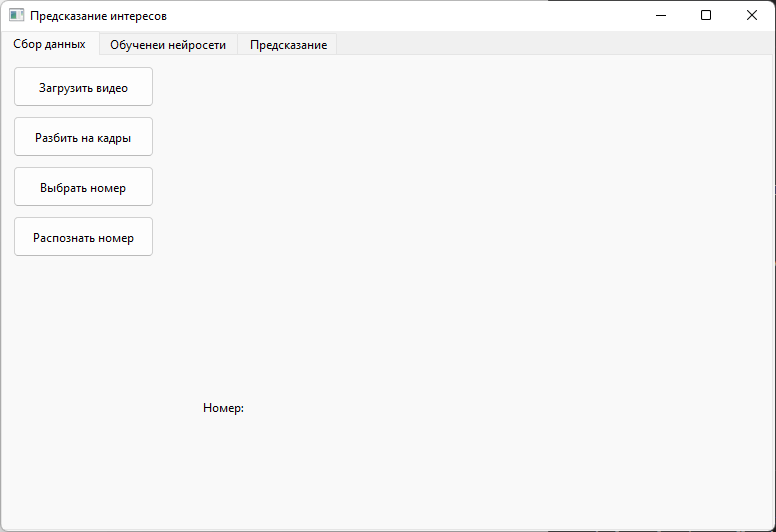
\includegraphics[width=0.5\textwidth]{window1}
	\caption{Окно программы}
	\label{f:window1}
\end{figure}

Выбор изображения представлен на рисунке~\ref{f:choose-pic}. Рядом с кнопками есть место для отрисовкм выбранного изображения.

\begin{figure}[h!]
	\centering
	\vspace{\toppaddingoffigure}
	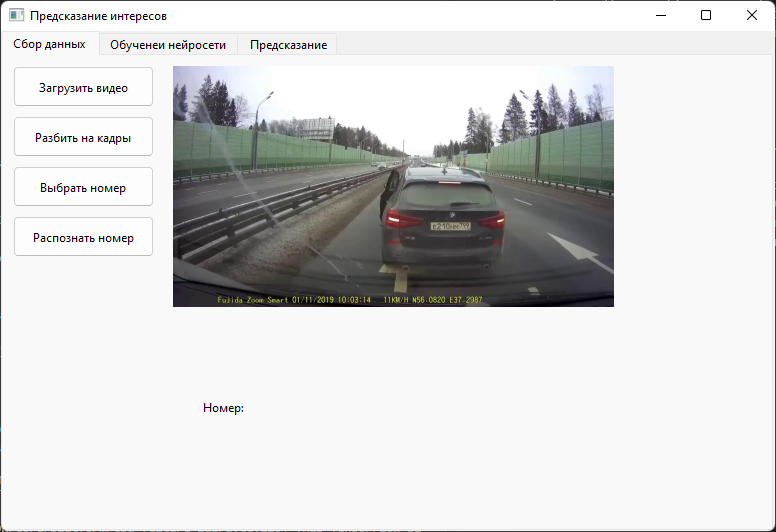
\includegraphics[width=0.5\textwidth]{choose-pic}
	\caption{Выбор изображения}
	\label{f:choose-pic}
\end{figure}

Распознавание номера представлено на рисунке~\ref{f:recognize}.

\begin{figure}[h!]
	\centering
	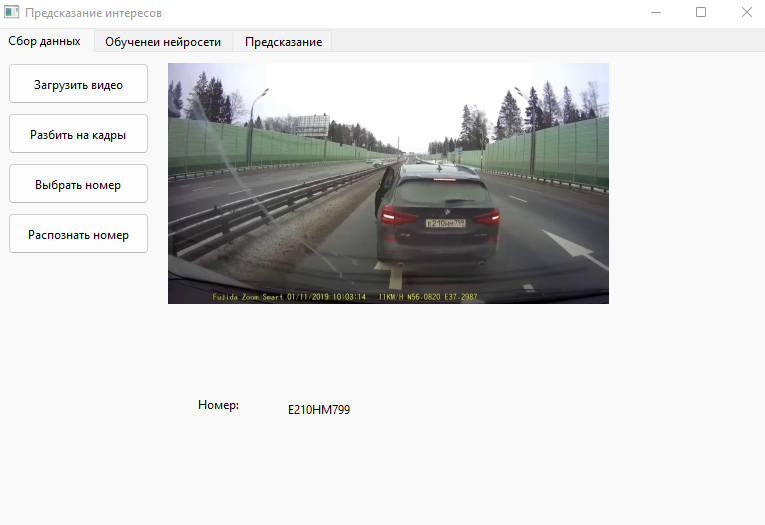
\includegraphics[width=0.5\textwidth]{recognize}
	\caption{Распознавание номера}
	\label{f:recognize}
\end{figure}


\newpage

Дальше происходит переход на сайт для определения модели автомобиля по распознанному номеру (рисунок~\ref{f:ident-model}).

\begin{figure}[h!]
	\centering
    \vspace{\toppaddingoffigure}
	
\includegraphics[width=0.5\textwidth]{ident-model}
	\caption{Определение модели авто}
	\label{f:ident-model}
\end{figure}


После этого предлагается выбрать изображение с бланком (рисунок~\ref{f:blank-examp}).

\begin{figure}[h!]
	\centering
	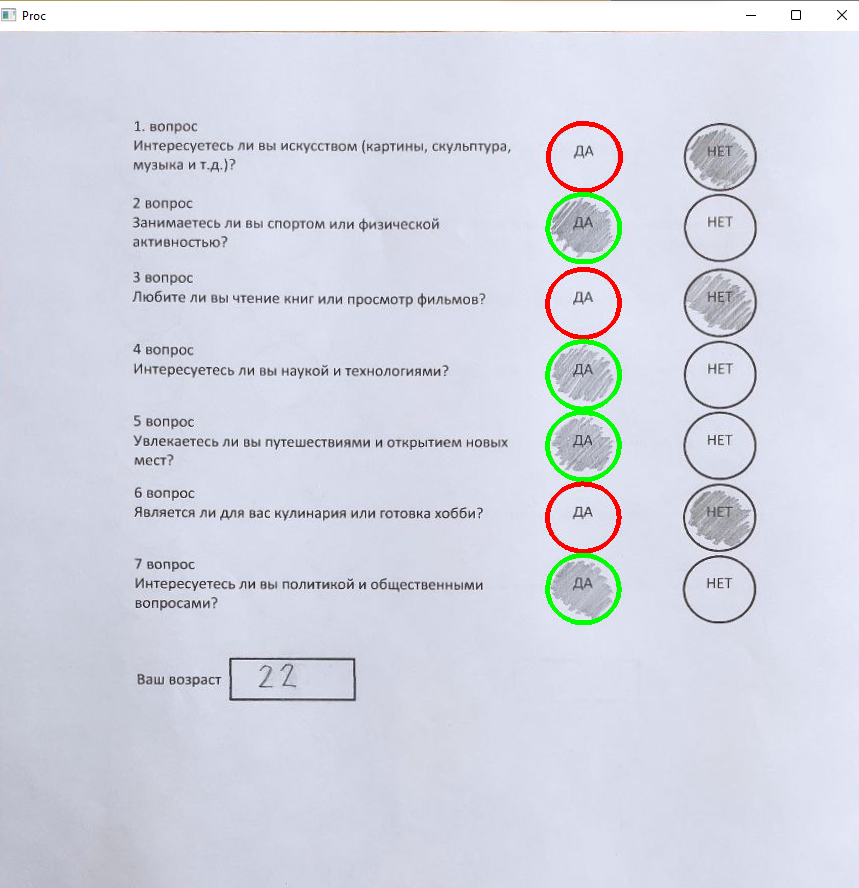
\includegraphics[width=0.5\textwidth]{blank-examp}
	\caption{Бланк опроса}
	\label{f:blank-examp}
\end{figure}


На бланке происходит обводка ответов. красным обводится в случае ответа НЕТ, а зеленым – в случае ответа ДА. Так же происходит считывание возраста, указанного в специальном поле.

Для удобства отладки происходит вывод в консоль (рисунок~\ref{f:console-log}).

\begin{figure}[h]
	\centering
	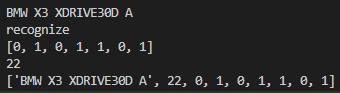
\includegraphics[width=0.5\textwidth]{console-log}
	\caption{Работа программы}
	\label{f:console-log}
\end{figure}

\newpage
Как можно увидеть по рисунку~\ref{f:console-log}, была определена модель автомобиля, так же выведен массив, содержащий ответы на вопросы. «0» означает ответ НЕТ, а «1» - ответ ДА. Кроме того, можно увидеть распознанный возраст «22». В конце все данные объединяются в единое целое, для записи в датасет – файл формата CSV. Результат записи представлен на рисунке~\ref{f:dataset}.

\begin{figure}[h!]
	\centering
    \vspace{\toppaddingoffigure}
	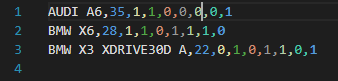
\includegraphics[width=0.5\textwidth]{dataset}
	\caption{Датасет}
	\label{f:dataset}
\end{figure}

\newpage
Окно для обучения нейросети представлено на рисунке~\ref{f:window2}. Имеются 2 кнопки дял выбора файла и начала обучения.

\begin{figure}[h!]
	\centering
    \vspace{\toppaddingoffigure}
	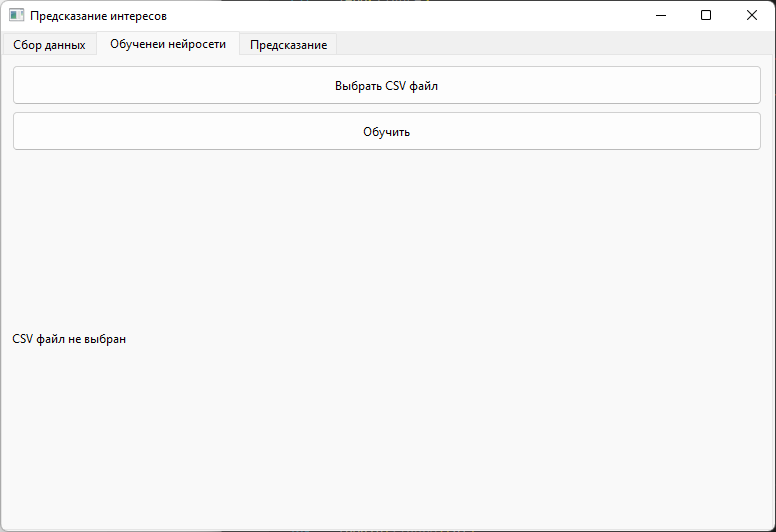
\includegraphics[width=0.5\textwidth]{window2}
	\caption{Окно программы}
	\label{f:window2}
\end{figure}

После выбора файла датасета выводится сообщение о выбранном файле (рисунок~\ref{f:window2.1}). Дальше можно приступать к обучению. По итогу обучения создается модель с расиширением ".keras".

\begin{figure}[h!]
	\centering
    \vspace{\toppaddingoffigure}
	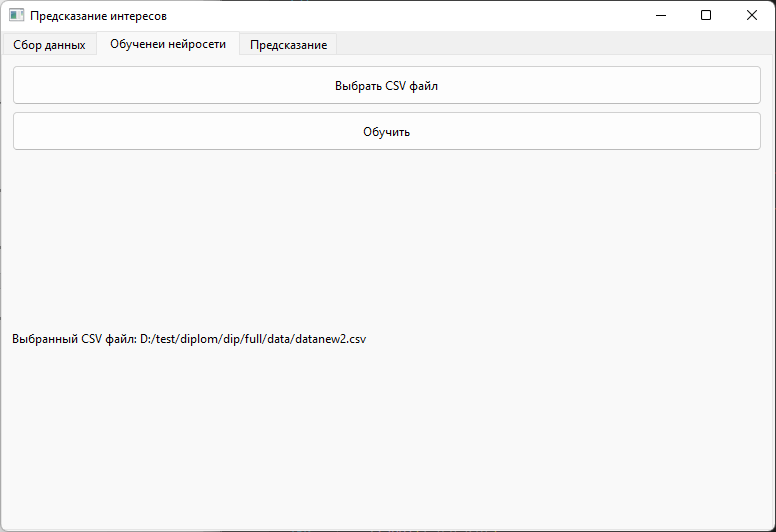
\includegraphics[width=0.5\textwidth]{window2.1}
	\caption{Окно программы}
	\label{f:window2.1}
\end{figure}

\newpage
Окно для предсказания интересов придставелно на рисунке~\ref{f:window3}.
\begin{figure}[h!]
	\centering
    \vspace{\toppaddingoffigure}
	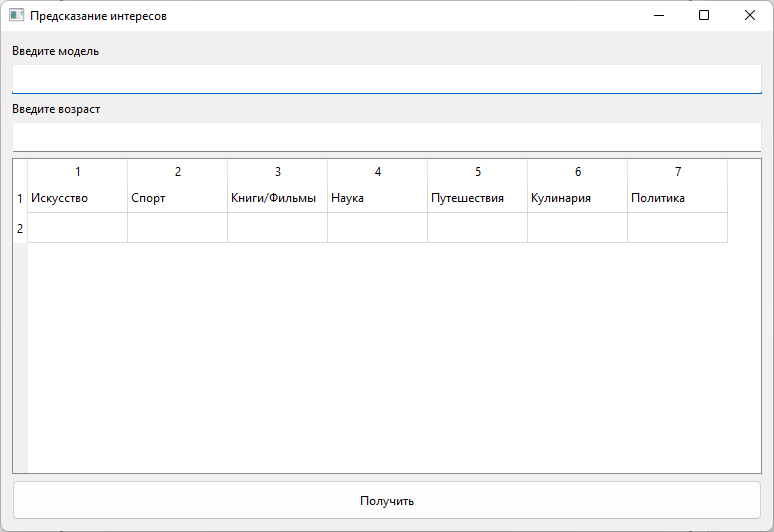
\includegraphics[width=0.5\textwidth]{window3}
	\caption{Окно программы}
	\label{f:window3}
\end{figure}

В поля для ввода необходимо ввести данные: название автомобиля и возраст владельца. После этого нажать на кнопку внизу экрана. Дальше модуль проведет работу, используя обученную модель для прогнозирования интересов. Результат работы представлен на рисунке~\ref{f:res-mod-pred}.
\begin{figure}[h!]
	\centering
    \vspace{\toppaddingoffigure}
	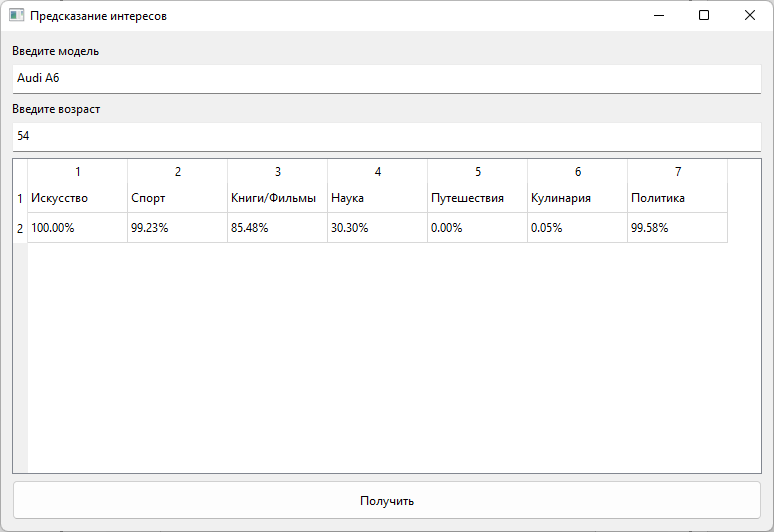
\includegraphics[width=0.5\textwidth]{res-mod-pred}
	\caption{Результат работы модуля}
	\label{f:res-mod-pred}
\end{figure}




\newpage
\section*{Выводы}
В двнном разделе были описаны основные технологии, которые использовались при разработке модулей, из которых состоит система. Было дано пояснение к основным функциям, а также расписан порядок их выполнения.
\newpage

\csection{Заключение}

В ходе выполнения проекта был разработан программная система, которая позволяет собирать информацию об интересах посетителей парковки и прогнозировать эти интересы. Для этого было использовано машинное обучение, методы компьютерного зрения и обработки опросных данных. 

Основной целью проекта было создать систему, которая поможет маркетологам анализировать интересы клиентов.

В процессе работы был проведен анализ предметной области, выявлены актуальность темы и ключевые требования. Были рассмотрены методы анализа данных, машинного обученияя и принцыпы копьютерного зрения.

Для реализации функционала были разработаны следующие компоненты: анализатор бланков, поиск модели автомобиля и распознавание номера. Кроме того были созданы скрипты для обучения нейронной сети с автоматизированным подбором гиперпараметров, а также для работы с обученной моделью. С помощью библиотеки-тюнера были подобраны наилучшие параметры для обучения и выбора оптимальной структуры нейронной сети.

Анализатор бланков позволяет автоматически обрабатывать изображения анкет, извлекать информацию об ответах на вопросы и возрасте. Для этого используются технологии обработки изображений и распознавания текста.

Компонент поиска модели автомобиля обеспечивает автоматизированный доступ к информации о моделях автомобилей. Для этого используется взаимодействие с сайтом, предоставляющим данные о транспортных средствах.

Компонент распознавания номера автомобиля служит для определения номера на изображении. Для этого используется предобученная модель машинного обучения.

В результате работы была разработана программная система, которая может быть использована в реальных задачах, направленных на анализ интересов посетителей парковок. Разработанная система принесет пользу для маркетологов и 
других людей, котороые работают с клиентами. Она помогает легко собирать и анализировать информацию о том, что нравится посетителям парковки. Это позволяет более точно нацеливать 
рекламные компании и предложения, что, в свою очередь, улучшает впечателния клиентов и делает маркетинг более эффективным.
% \newpage

\docappendix{Библиографический список}

\begin{references}
	\item\label{ref:num-methods} Бахвалов Н.С., Жидков Н.П., Кобельников Г.М.
	Численные методы [Текст] – 4-е изд. – М:. БИНОМ. Лаборатория
	знаний, 2006. – 636 с.: ил.
	\item Безрученко Б.П., Смирнов Д.А.
	Статистическое моделирование по временным рядам [Электронный ресурс]
	Cарат. отд-ние Ин-та радиотехники и электроники РАН.
	– Электрон. дан. – Саратов, 2000. – Режим доступа:
	http://www.masters.donntu.edu.ua/2012/fknt/dorosh/library/article4.pdf,
	свободный. - Загл. с экрана.
	\item Перельмутер А.В. Расчетные модели сооружений и возможность их анализа [Текст] / А.В. Перельмутер, В.И.
	Сливкер. Киев: Сталь, 2002. 600 с.
	\item NeuroShell 2 [Электронный ресурс] – Режим доступа: http://www.neuroproject.ru/aboutproduct.php, свободный. –
	Загл. с экрана.
	\item\label{ref:time-series-analysis} Бокс Дж., Дженкинс Г. Анализ временных рядов.
	Прогноз и управление [Текст]. - М.: Мир, 1974.

	\label{ref:total}
\end{references}

\docappendix{Авторская справка}\label{ax:authornote}
\input{pages/authornote.example.tex}


\docappendix{Листинг кода}\label{ax:code}

\begin{lstlisting}
    # Component for searching car models using the autoteka.ru website 
    from selenium import webdriver
    from selenium.webdriver.common.keys import Keys
    from selenium.webdriver.common.by import By
    from selenium.webdriver.support.ui import WebDriverWait  # Импортируем WebDriverWait
    from selenium.webdriver.support import expected_conditions as EC
    import time

    # Path to driver
    driver_path = 'drv/chromedriver-win64/chromedriver.exe'

    # URL link to the page
    website_url = 'https://autoteka.ru/'

    # Initializing the driver
    chrome_service = webdriver.chrome.service.Service(driver_path)
    driver = webdriver.Chrome(service=chrome_service)

    # Function for parsing
    def site(number):
        input = number
        driver.get(website_url)

        input_field = driver.find_element(By.NAME, 'identifier')
        input_field.send_keys(input)
        input_field.send_keys(Keys.ENTER)

        WebDriverWait(driver, 15).until(EC.url_changes(website_url))

        time.sleep(5)

        text_element = driver.find_element(By.CLASS_NAME, 'pit4K')
        text = text_element.text

        time.sleep(3)

        lines = text.split('\n')
        result = ' '.join(lines[:2])

        driver.quit()

        return result.split(',')[0].strip()
\end{lstlisting}

\begin{lstlisting}
    # Component for analyzing forms
    from imutils.perspective import four_point_transform
    from imutils import contours
    import numpy as np
    import argparse
    import imutils
    import cv2
    import csv
    import re
    import pytesseract
    
    # Define the correct answers for the exam (placeholder)
    ANSWER_KEY = {0: 0, 1: 0, 2: 0, 3: 0, 4: 0, 5: 0, 6: 0}
    
    # Path to Tesseract executable
    pytesseract.pytesseract.tesseract_cmd = r'C:\\Program Files\\Tesseract-OCR\\tesseract.exe'
    
    # Tesseract OCR configuration
    custom_config = r'--oem 3 --psm 6'
    
    def process_exam(image_path):
        # Read the input image
        image = cv2.imread(image_path)
        
        # Convert the image to grayscale
        gray = cv2.cvtColor(image, cv2.COLOR_BGR2GRAY)
        
        # Apply GaussianBlur to reduce noise and detail in the image
        blurred = cv2.GaussianBlur(gray, (5, 5), 0)
        
        # Use Canny edge detector to find edges in the image
        edged = cv2.Canny(blurred, 75, 200)
    
        # Find contours in the edged image
        cnts = cv2.findContours(edged.copy(), cv2.RETR_EXTERNAL, cv2.CHAIN_APPROX_SIMPLE)
        cnts = imutils.grab_contours(cnts)
        docCnt = None
    
        # Ensure at least one contour was found
        if len(cnts) > 0:
            # Sort the contours by area, keeping only the largest one
            cnts = sorted(cnts, key=cv2.contourArea, reverse=True)
            for c in cnts:
                # Approximate the contour
                peri = cv2.arcLength(c, True)
                approx = cv2.approxPolyDP(c, 0.02 * peri, True)
                
                # If the approximated contour has four points, assume it's the paper
                if len(approx) == 4:
                    docCnt = approx
                    break
    
        # Apply a perspective transform to obtain a top-down view of the paper
        paper = four_point_transform(image, docCnt.reshape(4, 2))
        warped = four_point_transform(gray, docCnt.reshape(4, 2))
    
        # Apply a binary threshold to the warped image
        thresh = cv2.threshold(warped, 0, 255, cv2.THRESH_BINARY_INV | cv2.THRESH_OTSU)[1]
    
        # Find contours in the thresholded image
        cnts = cv2.findContours(thresh.copy(), cv2.RETR_EXTERNAL, cv2.CHAIN_APPROX_SIMPLE)
        cnts = imutils.grab_contours(cnts)
        questionCnts = []
    
        # Loop over the contours
        for c in cnts:
            (x, y, w, h) = cv2.boundingRect(c)
            ar = w / float(h)
            
            # Filter the contours to find those that correspond to question bubbles
            if (w >= 50) and (h >= 50) and (ar >= 0.9) and (ar <= 1.1):
                questionCnts.append(c)
    
        # Sort the question contours top-to-bottom
        questionCnts = contours.sort_contours(questionCnts, method="top-to-bottom")[0]
        results = []
    
        # Loop over the question groups
        for (q, i) in enumerate(np.arange(0, len(questionCnts), 2)):
            cnts = contours.sort_contours(questionCnts[i:i + 2])[0]
            bubbled = None
            question_result = 0
    
            # Loop over the sorted contours
            for (j, c) in enumerate(cnts):
                mask = np.zeros(thresh.shape, dtype="uint8")
                cv2.drawContours(mask, [c], -1, 255, -1)
    
                mask = cv2.bitwise_and(thresh, thresh, mask=mask)
                total = cv2.countNonZero(mask)
                if bubbled is None or total > bubbled[0]:
                    bubbled = (total, j)
    
            color = (0, 0, 255)
            k = ANSWER_KEY[q]
    
            if k == bubbled[1]:
                question_result = 1
                color = (0, 255, 0)
    
            cv2.drawContours(paper, [cnts[k]], -1, color, 3)
            results.append(question_result)
    
        print(results)
    
        cv2.imshow("Proc", paper)
        cv2.waitKey(0)
    
        return results
    
    def get_age(image_path):
        # Read the input image
        image = cv2.imread(image_path)
        
        # Convert the image to grayscale
        gray = cv2.cvtColor(image, cv2.COLOR_BGR2GRAY)
        
        # Apply GaussianBlur to reduce noise and detail in the image
        blurred = cv2.GaussianBlur(gray, (5, 5), 0)
        
        # Use Canny edge detector to find edges in the image
        edged = cv2.Canny(blurred, 75, 200)
    
        # Find contours in the edged image
        cnts = cv2.findContours(edged.copy(), cv2.RETR_EXTERNAL, cv2.CHAIN_APPROX_SIMPLE)
        cnts = imutils.grab_contours(cnts)
        docCnt = None
    
        # Ensure at least one contour was found
        if len(cnts) > 0:
            # Sort the contours by area, keeping only the largest one
            cnts = sorted(cnts, key=cv2.contourArea, reverse=True)
            for c in cnts:
                # Approximate the contour
                peri = cv2.arcLength(c, True)
                approx = cv2.approxPolyDP(c, 0.02 * peri, True)
                
                # If the approximated contour has four points, assume it's the paper
                if len(approx) == 4:
                    docCnt = approx
                    break
    
        # Apply a perspective transform to obtain a top-down view of the paper
        paper = four_point_transform(image, docCnt.reshape(4, 2))
    
        # Further process the transformed image to find the age
        gray = cv2.cvtColor(paper, cv2.COLOR_BGR2GRAY)
        blurred = cv2.GaussianBlur(gray, (5, 5), 0)
        edged = cv2.Canny(blurred, 75, 200)
    
        cnts = cv2.findContours(edged.copy(), cv2.RETR_EXTERNAL, cv2.CHAIN_APPROX_SIMPLE)
        cnts = imutils.grab_contours(cnts)
        docCnt = None
    
        if len(cnts) > 0:
            cnts = sorted(cnts, key=cv2.contourArea, reverse=True)
            for c in cnts:
                peri = cv2.arcLength(c, True)
                approx = cv2.approxPolyDP(c, 0.02 * peri, True)
                if len(approx) == 4:
                    docCnt = approx
                    break
    
        paper = four_point_transform(paper, docCnt.reshape(4, 2))
    
        gray = cv2.cvtColor(paper, cv2.COLOR_BGR2GRAY)
        thresh = cv2.threshold(gray, 0, 255, cv2.THRESH_BINARY_INV | cv2.THRESH_OTSU)[1]
        
        # Use OCR to extract text from the thresholded image
        text = pytesseract.image_to_string(thresh, config=custom_config)
        
        # Find all two-digit numbers in the extracted text
        number = re.findall(r'\b\d+\b', text)
        two_digit_numbers = ' '.join(num for num in number if len(num) == 2)
        print(two_digit_numbers)
        return two_digit_numbers
    
    def write_to_csv(filename, results):
        # Append the results to a CSV file
        with open(filename, mode='a', newline='') as file:
            writer = csv.writer(file)
            writer.writerow(results)
    
    def blank(path_in, path_out, model):
        print(path_in)
        print(path_out)
        
        # Process the exam and get the age
        results = process_exam(path_in)
        age = get_age(path_in)
        
        # Insert model and age to the results
        results.insert(0, int(age))
        results.insert(0, model)
        
        print(results)
        write_to_csv(path_out, results)
        print("done")
    
    def main():
        # Set up argument parser
        ap = argparse.ArgumentParser()
        ap.add_argument("-i", "--image", required=True, help="path to the input image")
        ap.add_argument("-o", "--output", required=True, help="path to save the output CSV file")
        args = vars(ap.parse_args())
        
        # Process the exam and get the age
        results = process_exam(args["image"])
        age = get_age(args["image"])
        
        # Insert age to the results
        results.insert(0, int(age))
        print(results)
        
        # Write results to the CSV file
        write_to_csv(args["output"], results)
    
    if __name__ == "__main__":
        main()    
\end{lstlisting}

\begin{lstlisting}
    # Component for working with a trained model
    import numpy as np
    import pandas as pd
    import tensorflow as tf
    from sklearn.preprocessing import OneHotEncoder
    import os

    # Transforming new data
    def preprocess_new_data(new_data, full_data):
        # Convert categorical column "Model" to numeric values ​​using OneHotEncoding
        encoder = OneHotEncoder()
        encoder.fit(full_data[['Model']])
        model_encoded = encoder.transform(new_data[['Model']]).toarray()
        
        # Normalization of numerical data (age)
        age = new_data[['Age']].values
        age_normalized = (age - np.mean(full_data['Age'])) / np.std(full_data['Age'])

        # Merging the transformed data
        X_new = np.concatenate([age_normalized, model_encoded], axis=1)
        
        return X_new

    # Receiving Predictions
    def get_predictions(X_new, model_p):
        predictions = model_p.predict(X_new)
        # binary_predictions = np.round(predictions)
        return predictions

    # Output results
    def print_results(binary_predictions):
        # print("New data:")
        # print(new_data)
        print("\nPredictions:")
        np.set_printoptions(threshold=np.inf)
        print(binary_predictions)

    def main(model, age, model_pred):
        
        # Example of new data for testing
        new_data = pd.DataFrame({'Model': [model], 'Age': [int(age)]})

        # Transforming new data
        X_new = preprocess_new_data(new_data, full_data)

        if not os.path.isfile(model_pred):
            raise FileNotFoundError(f"Файл {model_pred} не найден")

        # Check file extension
        if not model_pred.endswith('.keras'):
            raise ValueError("Неправильный формат файла. Ожидался файл с расширением .keras")

        model_p = tf.keras.models.load_model(model_pred)

        # Getting predictions for just one example
        binary_predictions = get_predictions(X_new, model_p)

        art_prediction = binary_predictions[0][0]
        sport_prediction = binary_predictions[0][1]
        book_films_prediction = binary_predictions[0][2]
        science_prediction = binary_predictions[0][3]
        travel_prediction = binary_predictions[0][4]
        cooking_prediction = binary_predictions[0][5]
        politics_prediction = binary_predictions[0][6]

        # Writing to an array
        predictions_array = [art_prediction, sport_prediction, book_films_prediction, science_prediction, travel_prediction, cooking_prediction, politics_prediction]

        return predictions_array
\end{lstlisting}

\begin{lstlisting}
    # Component for training neural networks
    import pandas as pd
    import numpy as np
    import tensorflow as tf
    from tensorflow import keras
    from sklearn.model_selection import train_test_split, GridSearchCV
    from sklearn.preprocessing import OneHotEncoder
    from scikeras.wrappers import KerasClassifier
    from tensorflow.python.keras.callbacks import EarlyStopping, ModelCheckpoint
    from tqdm.keras import TqdmCallback

    # Load the dataset
    data = pd.read_csv('datanew2.csv')

    # Convert the categorical "Model" column to numerical values using OneHotEncoder
    encoder = OneHotEncoder()
    model_encoded = encoder.fit_transform(data[['Model']]).toarray()

    # Normalize the numerical "Age" column
    age = data[['Age']].values
    age_normalized = (age - np.mean(age)) / np.std(age)

    # Combine the normalized age data and the encoded model data
    X = np.concatenate([age_normalized, model_encoded], axis=1)

    # Extract the target variables (interests)
    y = data[['Art', 'Sport', 'Book/Films', 'Science', 'Travel', 'Cooking', 'Politics']].values

    # Split the data into training and test sets
    X_train, X_test, y_train, y_test = train_test_split(X, y, test_size=0.2, random_state=42)

    # Function to create the model with specified parameters
    def create_model(optimizer='adam', num_hidden_layers=2, num_neurons=20, activation='relu', dropout_rate=0.2, learning_rate=0.001):
        # Input layer
        inputs = tf.keras.Input(shape=(X.shape[1],))
        
        # First hidden layer
        x = tf.keras.layers.Dense(num_neurons, activation=activation)(inputs)
        x = tf.keras.layers.Dropout(dropout_rate)(x)
        
        # Additional hidden layers based on the parameter num_hidden_layers
        for _ in range(num_hidden_layers - 1):
            x = tf.keras.layers.Dense(num_neurons, activation=activation)(x)
            x = tf.keras.layers.Dropout(dropout_rate)(x)
        
        # Output layer with sigmoid activation for multi-label classification
        outputs = tf.keras.layers.Dense(7, activation='sigmoid')(x)
        
        # Create the model
        model = tf.keras.Model(inputs=inputs, outputs=outputs)
        
        # Set the optimizer based on the specified parameter
        if optimizer == 'adam':
            optimizer = tf.keras.optimizers.Adam(learning_rate=learning_rate)
        elif optimizer == 'rmsprop':
            optimizer = tf.keras.optimizers.RMSprop(learning_rate=learning_rate)
        elif optimizer == 'sgd':
            optimizer = tf.keras.optimizers.SGD(learning_rate=learning_rate)
        
        # Compile the model
        model.compile(optimizer=optimizer, loss='binary_crossentropy', metrics=['accuracy'])
        return model

    # Create a KerasClassifier with the create_model function
    model = KerasClassifier(model=create_model, verbose=0, epochs=100)

    # Define the grid of parameters for GridSearchCV
    param_grid = {
        'model__num_hidden_layers': [2, 3, 4, 5],
        'model__num_neurons': [20, 30, 40],
        'model__activation': ['relu', 'tanh'],
        'model__dropout_rate': [0.1, 0.2],
        'model__optimizer': ['adam', 'rmsprop', 'sgd'],
        'model__learning_rate': [0.001, 0.01, 0.1]
    }

    # Create a GridSearchCV object
    grid_search = GridSearchCV(estimator=model, param_grid=param_grid, cv=3, verbose=1, n_jobs=-1)

    # Fit the GridSearchCV object to the training data
    grid_search.fit(X_train, y_train)

    # Print the best parameters found by GridSearchCV
    print("Best: %f using %s" % (grid_search.best_score_, grid_search.best_params_))

    # Get the best parameters and create a model with them
    best_params = grid_search.best_params_
    best_model = create_model(
        optimizer=best_params['model__optimizer'],
        num_hidden_layers=best_params['model__num_hidden_layers'],
        num_neurons=best_params['model__num_neurons'],
        activation=best_params['model__activation'],
        dropout_rate=best_params['model__dropout_rate'],
        learning_rate=best_params['model__learning_rate']
    )

    # Define callbacks for early stopping, model checkpointing, and TQDM progress bar
    early_stopping = EarlyStopping(monitor='val_loss', patience=5, restore_best_weights=True)
    model_checkpoint = ModelCheckpoint('model.keras', save_best_only=True, monitor='val_loss', mode='min')
    tqdm_callback = TqdmCallback(verbose=1)

    # Train the best model with the callbacks
    history = best_model.fit(
        X_train, y_train,
        validation_split=0.2,
        epochs=100,
        callbacks=[early_stopping, model_checkpoint, tqdm_callback],
        verbose=0
    )

    # Evaluate the model on the test set
    loss, accuracy = best_model.evaluate(X_test, y_test)
    print(f'Test Accuracy: {accuracy}')
\end{lstlisting}

\begin{lstlisting}
    # Vehicle Number Plate Recognition Component
    import os
    from datetime import timedelta
    from pathlib import Path
    import matplotlib.pyplot as plt
    import cv2
    import numpy as np
    import re
    import imutils
    import pytesseract
    import pytesseract as tess
    tess.pytesseract.tesseract_cmd = r'Tesseract-OCR\tesseract.exe'
    from PyQt6 import uic
    from PyQt6.QtGui import QPixmap
    from PyQt6.QtWidgets import QApplication, QFileDialog, QMessageBox
    from imutils import contours
    from moviepy.editor import VideoFileClip
    import json
    import sqlite3
    import itertools
    import tensorflow as tf
    from skimage.feature import canny
    from skimage.transform import hough_line, hough_line_peaks, rotate
    from skimage.color import rgb2gray

    import matplotlib.gridspec as gridspec
    import cv2

    import autoteka
    import test_blank

    # Constants for saving frames per second from video
    SAVING_FRAMES_PER_SECOND = 1

    # Load the UI design file
    Form, Window = uic.loadUiType("Parking.ui")

    # Initialize the application and load the UI window
    app = QApplication([])
    window = Window()
    form = Form()
    form.setupUi(window)
    window.show()

    # Global variables to store the paths of video, image, and the result
    video_file = ''
    image_file = ''
    result = ''
    arr = []

    # Function to format the time delta for naming frames
    def format_timedelta(td):
        result = str(td)
        try:
            result, ms = result.split(".")
        except ValueError:
            return result + ".00".replace(":", "-")

        ms = round(int(ms) / 10000)
        return f"{result}.{ms:02}".replace(":", "-")

    # Function to load the video file
    def load():
        global video_file
        video_file = QFileDialog.getOpenFileName()
        path = Path(video_file[0])
        video_file = path.name
        print("load")

    # Function to split the video into frames
    def split():
        video_clip = VideoFileClip(video_file)
        filename, _ = os.path.splitext(video_file)

        if not os.path.isdir(filename):
            os.mkdir(filename)

        saving_frames_per_second = min(video_clip.fps, SAVING_FRAMES_PER_SECOND)
        step = 1 / video_clip.fps if saving_frames_per_second == 0 else 1 / saving_frames_per_second

        for current_duration in np.arange(0, video_clip.duration, step):
            frame_duration_formatted = format_timedelta(timedelta(seconds=current_duration)).replace(":", "-")
            frame_filename = os.path.join(filename, f"frame{frame_duration_formatted}.jpg")

            video_clip.save_frame(frame_filename, current_duration)
        print("split")

    # Function to check the format of the recognized license plate
    def check_format(variable):
        pattern = r'^[A-Z]\d{3}[A-Z]{2}\d{3}$'
        pattern2 = r'^[A-Z]\d{3}[A-Z]{2}\d{2}$'
        if re.match(pattern, variable) or re.match(pattern2, variable):
            return True
        else:
            return False

    # Function to choose an image file for recognition
    def choose():
        global image_file
        image_file = QFileDialog.getOpenFileName()
        image_file = image_file[0]
        form.label_6.setPixmap(QPixmap(image_file))
        form.label_6.setScaledContents(True)
        print("choose")

    # Function to recognize text from the car plate
    def carplate_text():
        global image_file

        image0 = cv2.imread(image_file)
        image_height, image_width, _ = image0.shape
        image = cv2.resize(image0, (1024, 1024))
        image = image.astype(np.float32)
        paths = 'model/recognize/model_resnet.tflite'
        interpreter = tf.lite.Interpreter(model_path=paths)
        interpreter.allocate_tensors()
        input_details = interpreter.get_input_details()
        output_details = interpreter.get_output_details()
        X_data1 = np.float32(image.reshape(1, 1024, 1024, 3))

        interpreter.set_tensor(input_details[0]['index'], X_data1)
        interpreter.invoke()
        detection = interpreter.get_tensor(output_details[0]['index'])
        net_out_value2 = interpreter.get_tensor(output_details[1]['index'])
        net_out_value3 = interpreter.get_tensor(output_details[2]['index'])
        net_out_value4 = interpreter.get_tensor(output_details[3]['index'])

        img = image0
        razmer = img.shape

        img2 = cv2.cvtColor(img, cv2.COLOR_BGR2RGB)
        img3 = img[:, :, :]

        number = 0
        while number < len(detection[0][number]) and detection[0, number, 0] > 0.9:
            number = number + 1

        box_x = int(detection[0, number, 0] * image_height)
        box_y = int(detection[0, number, 1] * image_width)
        box_width = int(detection[0, number, 2] * image_height)
        box_height = int(detection[0, number, 3] * image_width)

        cv2.rectangle(img2, (box_y, box_x), (box_height, box_width), (230, 230, 21), thickness=5)

        net_out_value3

        image = image0[box_x:box_width, box_y:box_height, :]
        img2 = cv2.cvtColor(image, cv2.COLOR_BGR2RGB)

        grayscale = rgb2gray(image)
        edges = canny(grayscale, sigma=3.0)
        out, angles, distances = hough_line(edges)
        h, theta, d = out, angles, distances
        angle_step = 0.5 * np.diff(theta).mean()
        d_step = 0.5 * np.diff(d).mean()
        bounds = [np.rad2deg(theta[0] - angle_step),
                np.rad2deg(theta[-1] + angle_step),
                d[-1] + d_step, d[0] - d_step]

        _, angles_peaks, _ = hough_line_peaks(out, angles, distances, num_peaks=20)
        angle = np.mean(np.rad2deg(angles_peaks))

        if 0 <= angle <= 90:
            rot_angle = angle - 90
        elif -45 <= angle < 0:
            rot_angle = angle - 90
        elif -90 <= angle < -45:
            rot_angle = 90 + angle
        if abs(rot_angle) > 20:
            rot_angle = 0

        rotated = rotate(image, rot_angle, resize=True) * 255
        rotated = rotated

        rotated1 = rotated[:, :, :]
        if rotated.shape[1] / rotated.shape[0] < 2:
            minus = np.abs(int(np.sin(np.radians(rot_angle)) * rotated.shape[0]))
            rotated1 = rotated[minus:-minus, :, :]
            print(minus)

        lab = cv2.cvtColor(rotated1, cv2.COLOR_BGR2LAB)
        l, a, b = cv2.split(lab)
        clahe = cv2.createCLAHE(clipLimit=3.0, tileGridSize=(8, 8))
        cl = clahe.apply(l)
        limg = cv2.merge((cl, a, b))
        final = cv2.cvtColor(limg, cv2.COLOR_LAB2BGR)

        letters = ['0', '1', '2', '3', '4', '5', '6', '7', '8', '9', 'A', 'B', 'C', 'E', 'H', 'K', 'M', 'O', 'P', 'T', 'X',
                'Y']

        def decode_batch(out):
            ret = []
            for j in range(out.shape[0]):
                out_best = list(np.argmax(out[j, 2:], 1))
                out_best = [k for k, g in itertools.groupby(out_best)]
                outstr = ''
                for c in out_best:
                    if c < len(letters):
                        outstr += letters[c]
                ret.append(outstr)
            return ret

        paths = 'model/recognize/model1_nomer.tflite'
        interpreter = tf.lite.Interpreter(model_path=paths)
        interpreter.allocate_tensors()

        input_details = interpreter.get_input_details()
        output_details = interpreter.get_output_details()
        img = final
        img = cv2.cvtColor(img, cv2.COLOR_BGR2GRAY)
        img = cv2.resize(img, (128, 64))
        img = img.astype(np.float32)
        img /= 255

        img1 = img.T
        img1.shape
        X_data1 = np.float32(img1.reshape(1, 128, 64, 1))
        input_index = (interpreter.get_input_details()[0]['index'])
        interpreter.set_tensor(input_details[0]['index'], X_data1)

        interpreter.invoke()

        net_out_value = interpreter.get_tensor(output_details[0]['index'])
        pred_texts = decode_batch(net_out_value)
        pred_texts

        fig = plt.figure(figsize=(10, 10))
        outer = gridspec.GridSpec(2, 1, wspace=10, hspace=0.1)
        ax1 = plt.Subplot(fig, outer[0])
        fig.add_subplot(ax1)
        ax2 = plt.Subplot(fig, outer[1])
        fig.add_subplot(ax2)
        return pred_texts[0]

    # Function to recognize the license plate and display information
    def recognize():
        global result
        result = carplate_text().upper()
        print(result)
        if result == '':
            QMessageBox.information(None, "Ошибка распознания", "НЕ РАСПОЗНАНО")
        elif check_format(result) != True:
            QMessageBox.information(None, "Ошибка формата", "Результат:" + result)
        else:
            form.label_7.setText(result)

            count = 0
            for i in range(len(arr)):
                if arr[i][0] == result:
                    count += 1

            if count == 0:
                arr.append([result, 1])
            else:
                for i in range(len(arr)):
                    if arr[i][0] == result:
                        arr[i][1] += 1

            for i in range(len(arr)):
                if arr[i][0] == result:
                    form.label_2.setText(str(arr[i][1]))
                    if arr[i][1] < 5:
                        form.label_5.setText('0%')
                    elif 5 <= arr[i][1] < 10:
                        form.label_5.setText('5%')
                    elif 10 <= arr[i][1] < 20:
                        form.label_5.setText('10%')
                    else:
                        form.label_5.setText('15%')
        
        model = autoteka.site(result)
        print(model)
        print("recognize")

        file_path, _ = QFileDialog.getOpenFileName()
        test_blank.blank(file_path, 'data/data.csv', model)

    # Connect UI buttons to their respective functions
    form.pushButton.clicked.connect(load)
    form.pushButton_2.clicked.connect(split)
    form.pushButton_3.clicked.connect(choose)
    form.pushButton_4.clicked.connect(recognize)

    # Start the application event loop
    app.exec()
\end{lstlisting}

\begin{lstlisting}
    #Interface
    # Importing necessary modules and libraries
    from PyQt6.QtWidgets import (
        QApplication, 
        QWidget, 
        QPushButton, 
        QLabel, 
        QVBoxLayout, 
        QTextEdit, 
        QTableWidget, 
        QTableWidgetItem,
        QTabWidget,
        QMainWindow,
        QFileDialog,
        QMessageBox
    )
    from PyQt6 import QtCore

    # Constant for saving frames per second from a video
    SAVING_FRAMES_PER_SECOND = 1

    # List of interest categories
    list_int = ["Искусство", "Спорт", "Книги/Фильмы", "Наука", "Путешествия", "Кулинария", "Политика"]

    # Global variables for storing file paths and results
    video_file = ''
    image_file = ''
    result = ''
    arr = []

    # Main window class inheriting from QMainWindow
    class MainWindow(QMainWindow):
        def __init__(self):
            super().__init__()

            self.setWindowTitle("Предсказание интересов")
            self.setGeometry(400, 250, 750, 500)

            # Creating a tab widget and setting it as the central widget
            self.tabs = QTabWidget()
            self.setCentralWidget(self.tabs)

            # Creating tabs
            self.create_tabs()

            self.model_pred = ""

        # Method to create tabs
        def create_tabs(self):
            # Creating the first tab for data collection
            tab1 = QWidget()
            
            self.pushButton = QPushButton(tab1)
            self.pushButton.setGeometry(QtCore.QRect(10, 10, 141, 41))
            self.pushButton.setObjectName("pushButton")
            self.pushButton.clicked.connect(self.load)
            self.pushButton.setText("Загрузить видео")

            self.pushButton_2 = QPushButton(tab1)
            self.pushButton_2.setGeometry(QtCore.QRect(10, 60, 141, 41))
            self.pushButton_2.setObjectName("pushButton_2")
            self.pushButton_2.clicked.connect(self.split)
            self.pushButton_2.setText("Разбить на кадры")

            self.pushButton_3 = QPushButton(tab1)
            self.pushButton_3.setGeometry(QtCore.QRect(10, 110, 141, 41))
            self.pushButton_3.setObjectName("pushButton_3")
            self.pushButton_3.clicked.connect(self.choose)
            self.pushButton_3.setText("Выбрать номер")

            self.pushButton_4 = QPushButton(tab1)
            self.pushButton_4.setGeometry(QtCore.QRect(10, 160, 141, 41))
            self.pushButton_4.setObjectName("pushButton_4")
            self.pushButton_4.clicked.connect(self.recognize)
            self.pushButton_4.setText("Распознать номер")

            self.label_6 = QLabel(tab1)
            self.label_6.setGeometry(QtCore.QRect(170, 10, 441, 241))
            self.label_6.setText("")
            self.label_6.setAlignment(QtCore.Qt.AlignmentFlag.AlignCenter)
            self.label_6.setObjectName("label_6")

            self.label_3 = QLabel(tab1)
            self.label_3.setGeometry(QtCore.QRect(200, 340, 71, 21))
            self.label_3.setText("Номер:")
            self.label_3.setObjectName("label_3")

            self.label_7 = QLabel(tab1)
            self.label_7.setGeometry(QtCore.QRect(290, 340, 161, 31))
            self.label_7.setText("")
            self.label_7.setObjectName("label_7")

            # Creating the second tab for neural network training
            tab2 = QWidget()
            tab2_layout = QVBoxLayout()

            self.pushButton_csv = QPushButton(tab2)
            self.pushButton_csv.setText("Выбрать CSV файл")
            self.pushButton_csv.setFixedSize(750, 40)
            self.pushButton_csv.clicked.connect(self.choose_csv_file)
            tab2_layout.addWidget(self.pushButton_csv)

            self.pushButton_learn = QPushButton(tab2)
            self.pushButton_learn.setText("Обучить")
            self.pushButton_learn.setFixedSize(750, 40)
            self.pushButton_learn.clicked.connect(self.learn)
            tab2_layout.addWidget(self.pushButton_learn)

            self.label_csv = QLabel(tab2)
            self.label_csv.setText("CSV файл не выбран")
            tab2_layout.addWidget(self.label_csv)

            tab2.setLayout(tab2_layout)

            # Creating the third tab for prediction
            tab3 = QWidget()
            tab3_layout = QVBoxLayout()

            self.label_model = QLabel('Введите модель', tab3)
            self.label_age = QLabel('Введите возраст', tab3)

            self.text_edit_model = QTextEdit(tab3)
            self.text_edit_model.setFixedSize(750, 30)
            
            self.text_edit_age = QTextEdit(tab3)
            self.text_edit_age.setFixedSize(750, 30)

            self.table = QTableWidget(tab3)
            self.table.setColumnCount(7)
            self.table.setRowCount(2)

            for col in range(7):
                item = QTableWidgetItem(list_int[col])
                self.table.setItem(0, col, item)

            self.button_predict = QPushButton('Получить', tab3)
            self.button_predict.setFixedSize(750, 40)
            self.button_predict.clicked.connect(self.proc)

            self.button_choose_file = QPushButton('Выбрать файл модели', tab3)
            self.button_choose_file.setFixedSize(750, 40)
            self.button_choose_file.clicked.connect(self.choose_model_file)

            # Adding widgets to the third tab
            tab3_layout.addWidget(self.label_model)
            tab3_layout.addWidget(self.text_edit_model)
            tab3_layout.addWidget(self.label_age)
            tab3_layout.addWidget(self.text_edit_age)
            tab3_layout.addWidget(self.button_choose_file)
            tab3_layout.addWidget(self.table)
            tab3_layout.addWidget(self.button_predict)

            tab3.setLayout(tab3_layout)

            # Adding tabs to the QTabWidget
            self.tabs.addTab(tab1, "Сбор данных")
            self.tabs.addTab(tab2, "Обучение нейросети")
            self.tabs.addTab(tab3, "Предсказание")

        # Placeholder method for learning
        def learn(path):
            pass

        # Method to choose a CSV file
        def choose_csv_file(self):
            file_dialog = QFileDialog()
            options = file_dialog.options()
            file_name, _ = QFileDialog.getOpenFileName(self, "Выберите CSV файл", "", "CSV Files (*.csv);;All Files (*)", options=options)
            if file_name:
                self.csv_file = file_name
                self.label_csv.setText(f"Выбранный CSV файл: {file_name}")
            print(self.csv_file)

        # Method to choose a model file
        def choose_model_file(self):
            file_dialog = QFileDialog()
            options = file_dialog.options()
            file_name, _ = QFileDialog.getOpenFileName(self, "Выберите файл модели", "", "Model Files (*.keras);;All Files (*)", options=options)
            if file_name:
                self.model_pred = file_name 
            print(self.model_pred)
            
        # Method to process the model and age input and get predictions
        def proc(self):
            model = self.text_edit_model.toPlainText()
            age = self.text_edit_age.toPlainText()
            if (model != "") & (age != "") & (self.model_pred != ""):
                predictions = test_single.main(model, age, self.model_pred)
                print(predictions)
                for col in range(7):
                    predictions[col] = float(predictions[col])
                    item = QTableWidgetItem(str("{:2.2f}".format(predictions[col] * 100)) + "%")
                    self.table.setItem(1, col, item)

    if __name__ == "__main__":
        app = QApplication(sys.argv)
                
        window = MainWindow()
        window.show()
                
        sys.exit(app.exec()) 
\end{lstlisting}


\docappendix[Справочное]{Библиографический список}

\begin{references}
	\item\label{ref:data-collection} Data Collection [Электронный ресурс] – Режим доступа: https://www.tutorialspoint.com/data-collection, свободный. – Загл. с экрана.

	\item\label{ref:data-analysis} Анализ данных [Электронный ресурс] – Режим доступа: https://en.wikipedia.org/wiki/Data\_analysis, свободный. – Загл. с экрана.

	\item\label{ref:data-visualization} Визуализация данных [Электронный ресурс] – Режим доступа: https://practicum.yandex.ru/blog/vizualizaciya-dannyh/, свободный. – Загл. с экрана.

	\item\label{ref:machine-learning} Машинное обучение: методы и способы [Электронный ресурс] – Режим доступа: https://www.osp.ru/cio/2018/05/13054535, свободный. – Загл. с экрана.

	\item\label{ref:marketing} Медведев П.М. Организация маркетинговой службы с нуля [Текст] ЗАО Издательский дом «Питер». 2005. – 224 с.: ил.

	\item\label{ref:res-net} Exploring ResNet50: An In-Depth Look at the Model Architecture and Code Implementation [Электронный ресурс] – Режим доступа: https://medium.com/@nitishkundu1993/exploring-resnet50-an-in-depth-look-at-the-model-architecture-and-code-implementation-d8d8fa67e46f, свободный. – Загл. с экрана.

	\item\label{ref:cnn-lstm} CNN-LSTM Architecture and Image Captioning [Электронный ресурс] – Режим доступа: https://medium.com/analytics-vidhya/cnn-lstm-architecture-and-image-captioning-2351fc18e8d7, свободный. – Загл. с экрана.
	
	\item\label{ref:neuron} Дюк В.А., Флегонтов А.В., Фомина И.К. Применение технологий интеллектуального анализа данных в естественнонаучных, технических и гуманитарных областях [Текст] Известия Российского государственного педагогического университета им. А.И. Герцена. 2011. No 138.

	\item\label{ref:back-error} Метод обратного распространения ошибки [Электронный ресурс] – Режим доступа: https://education.yandex.ru/handbook/ml/article/metod-obratnogo-rasprostraneniya-oshibki, свободный. – Загл. с экрана.

	\item\label{ref:neuron-model} Neurons in Neural Networks [Электронный ресурс] – Режим доступа: https://www.baeldung.com/cs/neural-networks-neurons, свободный. – Загл. с экрана.

	\item\label{ref:nbc} Наивный байесовский классификатор [Электронный ресурс] – Режим доступа: https://ru.wikipedia.org/wiki/Наивный\_байесовский\_классификатор, свободный. – Загл. с экрана.

	\item\label{ref:log-reg} Пампел Фред, Цвиркун Дмитрий, Груздев Артем. Логистическая регрессия [Текст] ДМК-Пресс, 2023 г. – 218 с.: ил.

	
	\label{ref:total}
\end{references}



}

}

}

% Установка рамок
\ifthenelse{\boolean{setframes}}{
	% Устанавливаем главную рамку для одной страницы
	\tocloftpagestyle{mainframe}

	% Устанавливаем рамку страниц, которая будет отрисовываться после главной
	\pagestyle{pageframe}}{
	\tocloftpagestyle{empty}\renewcommand{\cftaftertoctitle}{\hfill}}
% Меняем размер нижнего отступа до текста, чтобы текст до рамки страниц был 10mm.
% Рамка страниц имеет меньшую высоту содержимого нижней таблицы.
\addtolength{\textheight}{+25mm}
% Устанавливаем "Содержание", включающее в себя описание разделов документа
\tableofcontents\newpage

% Подключаем содержимое документа
\IfFileExists{./pages/content.tex} {
	% Привер файла содержимого документа
% Измените подключаемые файлы в зависимости от вашей структуры документа


\csection{Введение}

В современном мире сбор и анализ данных играют ключевую роль в принятии решений во многих сферах деятельности. 
Благодаря развитию технологий, стало возможным эффективно использовать огромные объемы данных для улучшения 
различных процессов и повышения эффективности работы. В особенности, методы компьютерного зрения и искусственного 
интеллекта открывают новые возможности для автоматизации и оптимизации задач, которые ранее выполнялись вручную.

С развитием технологий обработки данных и машинного обучения, особенно нейронных сетей, стало возможным решать 
сложные задачи, такие как распознавание образов, анализ поведения, предсказания исходов каких-любо событи и так далее. 
Эти технологии находят широкое применение в самых разных областях, от маркетинга и розничной 
торговли до здравоохранения и транспорта.

Современные маркетологи сталкиваются с необходимостью глубоко понимать интересы и предпочтения своих клиентов, чтобы создавать эффективные стратегии и кампании. Проект по автоматизации процесса сбора и анализа интересов клиентов автостоянки предоставляет маркетологам мощный инструмент для достижения этой цели.

Благодаря полученным данным, маркетологи смогут более точно сегментировать аудиторию, разрабатывать персонализированные предложения и эффективно проводить рекламные кампании. Это приведет к улучшению взаимодействия с клиентами, увеличению их лояльности и, в конечном итоге, к росту продаж и прибыли компании.

Исходя из выше сказанного, было принято решение о создании системы, которая смогла бы автоматизировать процесс сбора и 
анализа интересов клиентов автостоянки, для того чтобы предоставить пользователям информацию о посетителях.

\pagebreak


\section{Анализ предметной области}

\subsection{Машина времени}

Машина времени является гипотетическим устройством, способным перемещаться во времени, обеспечивая возможность путешествия в прошлое или будущее. В связи с этим, анализ предметной области машины времени включает следующие аспекты:


\begin{enumerate}
	\item физические принципы: необходимо изучить теоретические основы, согласно которым могла бы функционировать машина времени. Это может включать обсуждение специальной теории относительности, черных дыр, петель времени и других концепций из физики;

	\item технические особенности: рассмотрим возможные способы построения и дизайна машины времени. Какие технологии или материалы могут быть использованы для ее создания? Какие опасности или препятствия могут возникнуть при ее конструировании?

	\item парадоксы времени: проанализируем различные парадоксы, которые могут возникнуть при использовании машины времени, такие как "парадокс дедушки" или "парадокс самовыполнения". Какие последствия они могут иметь для временных путешественников?

	\item этические и социальные аспекты: обсудим влияние машины времени на общество и индивидуума. Какие этические вопросы возникают при использовании данной технологии? Какие последствия она может иметь для личной и мировой истории?

	\item возможные приложения: рассмотрим потенциальные области применения машины времени, такие как исследования истории, изменение прошлого или будущего, предсказание событий и т. д.
\end{enumerate}

\subsection{Сравнение аналогов}

Машина времени 1:
\begin{itemize}
	\item перемещает человека в прошлое или будущее;
	\item имеет ограничение по количеству путешествий во времени;
	\item не поддерживает контроль точного места приземления.
\end{itemize}

Машина времени 2:
\begin{itemize}
	\item позволяет путешествовать во времени как в прошлое, так и в будущее;
	\item имеет более сложную систему навигации и управления;
	\item предоставляет дополнительные возможности и функции.
\end{itemize}

Машина времени 3:
\begin{itemize}
	\item позволяет точно указывать дату, время и место для путешествия;
	\item обладает самой передовой технологией и функционалом;
	\item эффективнее и безопаснее других машин времени.
\end{itemize}

Эти машины времени можно сравнивать через их уникальные особенности, функционал, надежность и возможности путешествия. Каждая из них обладает своими преимуществами и ограничениями, что делает их различными в использовани

В таблице \ref{t:comp-an} представлено сравнение аналагов.

\begin{table}[ht]

	\centering
	\Large
	\begin{threeparttable}
		\caption{Сравнение аналогов}
		\label{t:comp-an}
		\begin{tabularx}{\textwidth}{|X|c|c|c|}
			\hline
			Критерии \textbackslash\ Аналоги & Машина времени 1 & Машина времени 2 & Машина времени 3 \\
			\hline
			Критерий 1
			                                 & нет              & да               & да               \\
			\hline
			Критерий 2
			                                 & нет              & да               & да               \\
			\hline
			Критерий 3
			                                 & да               & да               & нет              \\
			\hline
			Критерий 4
			                                 & нет              & нет              & да               \\
			\hline
		\end{tabularx}
	\end{threeparttable}
	\vspace{\bottompaddingoftable}
\end{table}

Таким образом разработка машины времени является актуальной.

\section*{Выводы}


Анализ предметной области машины времени требует не только фантазии и творческого мышления, но и глубоких знаний в области физики, философии, этики и технологии.



\newpage

\section{Структура машины времени}

Структура машины времени представлена на рисунке~\ref{f:time-machine}.


\begin{figure}[ht]
	\centering
	\vspace{\toppaddingoffigure}
	
\includegraphics[width=0.7\textwidth]{time-machine}
	\caption{Структура машины времени}
	\label{f:time-machine}
\end{figure}


Разработка структуры машины времени является сложной задачей, поскольку такое устройство находится за пределами существующих научных и инженерных возможностей. Однако, если мы предположим, что машина времени возможна, то ее структура, вероятно, будет иметь следующие основные компоненты:

\begin{enumerate}
	\item часовой механизм: стандартный механизм, который управляет передвижением во времени, аналогично тому, как часовой механизм контролирует передвижение стрелок на циферблате часов;

	\item энергетический источник: мощный источник энергии, способный обеспечить работу машины времени и перемещение объектов во времени;

	\item контрольная система: комплекс алгоритмов и программного обеспечения, которые контролируют точное время и координируют перемещение во времени;

	\item защитные механизмы: системы, предотвращающие нежелательное перемещение во времени или обеспечивающие безопасность при использовании машины времени;

	\item интерфейс пользователя: устройства ввода и вывода, позволяющие пользователю программировать желаемые временные точки или координировать перемещение во времени;

	\item материалы и конструкция: специальные материалы и компоненты, обеспечивающие устойчивость и работоспособность машины времени.
\end{enumerate}

Хотя это очень упрощенное описание возможной структуры машины времени, это может помочь представить основные компоненты, которые потребуются для того, чтобы создать такое устройство. Однако необходимо помнить, что вышеописанная концепция является вымышленной и не имеет научного обоснования.


Пример ссылки на источник \refref{ref:num-methods}.

Пример еще ссылки на источник \refref{ref:time-series-analysis}.

Код представлен в приложении \ref{ax:code}.

Авторская справка представлена в приложении \ref{ax:authornote}.

Какое-то справочное приложение представлено в приложении \ref{ax:ref}.


\subsection{Расчёты}

Расчёты представлены ниже

\begin{gather}
	a = \tan(\frac{\alpha}{2})*a*\pi, \\
	\bigtriangleup b = \cos(\beta)*a, \\
	c = \sin{\beta}.
\end{gather}


\examplecommand

\newpage

\section{Программная реализация}
В данном разделе будут рассмотрены средства, методы и библиотеки, которые использовались при программной реализации. Кроме того, тут будут описаны основные функции, которые реализованы в модулях, и то как они работают. Так же будет рассмотрен процесс работы системы на заданном примере. 

Для наглядного описания взаимодействия разработанных компонентов ниже приведена диаграмма вариантов использования (рисунок~\ref{f:diag-comp}).

\begin{figure}[h!]
    \centering
    \vspace{\toppaddingoffigure}
    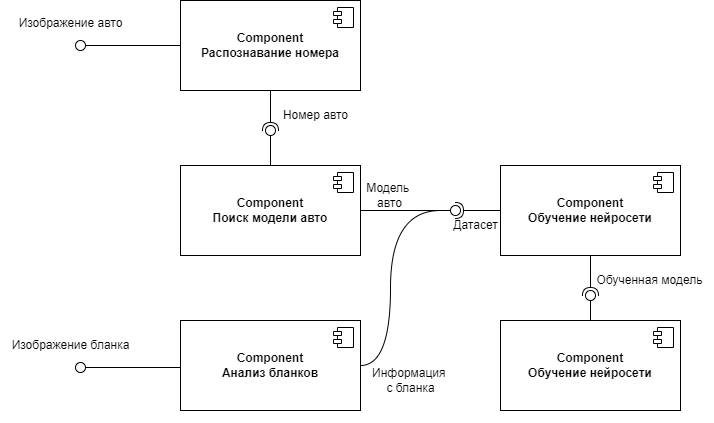
\includegraphics[width=0.8\textwidth]{diag-comp}
    \caption{Диаграмма компонентов}
    \label{f:diag-comp}
\end{figure}

\subsection{Программная реализация модуля для сбора данных}

В данном разделе рассматриваются технологии, используемые при реализации, и описывается сама программная реализация всех компонентов, которые выходят в модуль сбора данных.

\subsubsection{Анализ бланков}

В коде компонента используются библиотеки «cv2» (OpenCV) для обработки изображений, «numpy» для работы с массивами, «argparse» для обработки аргументов командной строки, «imutils» для удобных функций обработки изображений, «csv» для записи результатов в CSV-файл и «pytesseract» для распознавания текста на изображении.
Сам компонент имеет следующие основные функции:

\begin{enumerate}
    \item process\_exam(image\_path). Функция принимает путь к изображению листа. Используя библиотеку «cv2», выполняет следующие шаги обработки изображения:
        \begin{enumerate}
            \item преобразует изображение в оттенки серого, размывает его и применяет пороговое преобразование для выделения контуров;
            \item находит контуры на изображении и выбирает наибольший контур, который предположительно является контуром экзаменационного листа;
            \item используя функцию «four\_point\_transform» из «imutils», выполняет перспективное преобразование изображения, чтобы получить прямоугольный экзаменационный лист;
            \item применяет пороговое преобразование к преобразованному изображению и находит контуры вопросов на экзаменационном листе;
            \item для каждого вопроса находит наибольший контур, который предположительно является контуром выбранного ответа;
            \item определяет выбранные ответы и возвращает результаты в виде списка;
        \end{enumerate}
    \item get\_age(image\_path). Функция принимает путь к изображению документа, содержащего возраст. Используя библиотеку «cv2», выполняет следующие шаги обработки изображения:
        \begin{enumerate}
            \item находит контуры на изображении и выбирает наибольший контур, который предположительно является контуром документа;
            \item используя функцию «four\_point\_transform» из «imutils», выполняет перспективное преобразование изображения, чтобы получить прямоугольный документ;
            \item применяет пороговое преобразование к преобразованному изображению и находит контуры чисел на документе;
            \item используя библиотеку «pytesseract», выполняет распознавание текста на изображении и находит числа, представляющие возраст;
            \item возвращает возраст в виде строки;
        \end{enumerate}
    \item write\_to\_csv(filename, results):
        \begin{enumerate}
            \item функция принимает путь к CSV-файлу и результаты обработки;
            \item используя библиотеку «csv», открывает файл в режиме добавления и записывает результаты в виде строки в CSV-файл;
        \end{enumerate}
    \item blank(path\_in, path\_out, model):
        \begin{enumerate}
            \item функция принимает путь к входному изображению, путь к выходному CSV-файлу и модель (номер экзаменационного листа);
            \item вызывает функции «process\_exam» и «get\_age» для обработки изображения и определения возраста;
            \item добавляет модель и возраст в начало списка результатов;
            \item вызывает функцию «write\_to\_csv» для записи результатов в CSV-файл;
        \end{enumerate}
    \item main():
        \begin{enumerate}
            \item основная функция, которая принимает путь к входному изображению и путь к выходному CSV-файлу с помощью аргументов командной строки;
            \item вызывает функции «process\_exam» и «get\_age» для обработки изображения и определения возраста;
            \item вызывает функцию «write\_to\_csv» для записи результатов в CSV-файл;
        \end{enumerate}
\end{enumerate}

\subsubsection{Поиск модели авто}

При программной реализации данного компонента использовалась библиотеку Selenium для автоматизации веб-браузера. Она включает в себя следующие функции и шаги:
\begin{enumerate}
    \item импортируются необходимые модули: selenium, time, и другие модули, необходимые для работы с Selenium;
    \item указывается путь к драйверу браузера (chromedriver.exe) в переменной «driver\_path»;
    \item указывается URL-адрес веб-сайта, на котором будет выполняться поиск, в переменной «website\_url»;
    \item указывается номер, который будет использоваться в качестве вводного параметра, в переменной «num»;
    \item создается экземпляр браузера Chrome с использованием указанного драйвера в переменной «driver»;
    \item ­определяется функция «site», которая принимает в качестве аргумента номер и выполняет следующие действия:
        \begin{enumerate}
            \item загружается веб-страница с указанным URL-адресом;
            \item на странице вводится номер в поле с именем "identifier";
            \item номер отправляется в поле ввода с помощью метода «send\_keys» и клавиши Enter;
            \item ожидается изменение URL-адреса на веб-странице с использованием «WebDriverWait»;
            \item ожидается 3 секунды для загрузки страницы;
            \item мна странице находится элемент с классом "pit4K", который содержит текст, связанный с номером;
            \item текст из элемента извлекается и разбивается на строки;
            \item результирующий текст объединяется в две строки с помощью «join(lines[:2])»;
            \item возвращается первая строка текста, разделенная запятой и приводится к нижнему регистру;
            \item завершается работа браузера с помощью «driver.quit()»;
        \end{enumerate}
        \item в блоке «if \_\_name\_\_ == "\_\_main\_\_":» вызывается функция «site» с передачей номера в качестве аргумента и выводится результат в консоль.
    \end{enumerate}

\subsubsection{Распознавание номера}

Для работы модуля используются следующие библиотеки и модули:
    \begin{itemize}
        \item PyQt6. Для создания графического интерфейса пользователя и обработки событий;
        \item OpenCV. для обработки изображений и видео, включая разделение видео на кадры и обнаружение номерных знаков;
        \item TensorFlow Lite. Для загрузки и использования моделей машинного обучения для распознавания номеров автомобилей;
        \item NumPy. Для работы с массивами и математических операций;
        \item Matplotlib. Для визуализации результатов обработки изображений;
        \item SciPy. Для преобразования изображений и обнаружения линий;
        \item autoteka и test\_blank. Пользовательские модули для работы с сайтом и создания пустых бланков.
    \end{itemize}

    Функции компонента:
    \begin{enumerate}
        \item load():
            \begin{enumerate}
                \item функция загружает видеофайл из диалогового окна выбора файлов;
                \item использует метод QFileDialog.getOpenFileName() для открытия диалогового окна выбора файлов;
                \item путь к выбранному видеофайлу сохраняется в переменной video\_file в формате Path(video\_file[0]);
            \end{enumerate}
        \item split():
            \begin{enumerate}
                \item функция разделяет видеофайл на отдельные кадры;
                \item создает папку с именем, соответствующим имени исходного видеофайла, если такой папки еще нет;
                \item использует библиотеку moviepy для разделения видео на кадры с заданной частотой кадров (SAVING\_FRAMES\_PER\_SECOND);
                \item каждый кадр сохраняется в папке с именем, соответствующим времени его появления в видео;
            \end{enumerate}
        \item choose():
            \begin{enumerate}
                \item функция распознает номер автомобиля на изображении;
                \item использует модели машинного обучения для обнаружения номерного знака и его распознавания;
                \item производит предварительную обработку изображения, включая изменение размера, преобразование в оттенки серого, применение фильтра Canny для обнаружения границ и преобразование изображения в бинарное;
                \item использует модель TensorFlow Lite для распознавания символов на номерном знаке;
                \item возвращает распознанный номер автомобиля в виде строки;
            \end{enumerate}
        \item recognize():
            \begin{enumerate}
                \item функция вызывается при нажатии на кнопку "Распознать";
                \item вызывает функцию `carplate\_text()` для распознавания номера автомобиля на выбранном изображении;
                \item отображает результат распознавания на метке;
                \item обновляет статистику по количеству распознанных номеров и их вероятности;
                \item проверяет формат распознанного номера и выводит сообщение об ошибке, если формат неверный;
                \item если формат верный, сохраняет результат в массив `arr` и обновляет статистику на метках;
                \item передает полученный номер в компонент определения модели машины;   
            \end{enumerate} 
    \end{enumerate}


\subsection{Программная реализация модуля для обучения нейросети и предсказания интересов}

В данном разделе будет описана программная реализация всех компонентов. Модуль разрабатывался на языке Python в среде разработки Visual Studio Code.

\subsubsection{Обучение нейросети}
Этот скрипт реализует процесс обучения нейронной сети для прогнозирования интересов на основе их возраста и модели авто. При его создании использовались следующие средства:
\begin{itemize}
    \item библиотека pandas. Используется для работы с данными в формате DataFrame, включая загрузку данных из CSV-файла и их предварительную обработку;
    \item библиотека numpy. Применяется для работы с числовыми данными и выполнения математических операций, таких как нормализация числовых данных;
    \item библиотека scikit-learn. Используется для разделения данных на обучающий и тестовый наборы, преобразования категориальных переменных в числовые с помощью OneHotEncoding, подбора оптимальных параметров модели с помощью GridSearchCV и других методов машинного обучения;
    \item библиотека TensorFlow. Применяется для создания и обучения нейронных сетей. В данном скрипте используется Keras API для построения и компиляции модели нейронной сети.
\end{itemize}

Теперь более подробно рассмотрим процесс реализации:
\begin{enumerate}
    \item загрузка данных. Из CSV-файла 'datanew.csv' данные загружаются в объект DataFrame библиотеки pandas. Входными параметрами являются поля Model и Age, а поля Sport, book/films, Science, Travel, Cooking, Politics выходными.
    \item предобработка данных. Категориальный столбец "Model" преобразуется в числовые значения с помощью метода OneHotEncoding из библиотеки sklearn. Нормализация числовых данных о возрасте также выполняется для лучшей работы нейронной сети;
    \item разделение данных. Данные разделяются на обучающий и тестовый наборы с использованием функции train\_test\_split из библиотеки sklearn;
    \item определение функции создания модели. Функция create\_model определяет архитектуру нейронной сети с возможностью настройки различных параметров, таких как количество слоев, количество нейронов, функция активации, dropout rate, оптимизатор и т.д.;
    \item создание модели KerasClassifier. Создается модель KerasClassifier, обертка над моделью Keras, для использования с методом кросс-валидации GridSearchCV из библиотеки sklearn;
    \item задание сетки параметров для подбора. Задаются параметры для поиска лучших комбинаций параметров модели с помощью GridSearchCV;
    \item создание объекта GridSearchCV. Создается объект GridSearchCV с указанными параметрами для поиска оптимальных гиперпараметров модели;
    \item определение обратного вызова EarlyStopping. Обратный вызов EarlyStopping определяется для автоматической остановки обучения, если происходит переобучение модели;
    \item подгонка объекта GridSearchCV к данным. Объект GridSearchCV подгоняется к обучающим данным с использованием метода fit, включая обратный вызов EarlyStopping;
    \item вывод лучших параметров. Выводятся лучшие параметры модели, найденные с помощью GridSearchCV;
    \item оценка модели с лучшими параметрами. Лучшая модель из GridSearchCV оценивается на тестовом наборе данных, и выводится точность предсказания.
\end{enumerate}


\subsubsection{Реализация модуля}

При реализации модуля были написаны 2 скрипта. Один для выполнения предсказаний, другой реализует интерфейс. Использовались следующие средства:
\begin{itemize}
    \item PyQt6. PyQt6 является набором библиотек для Python, предоставляющим интерфейс для работы с графическими приложениями на основе Qt, кросс-платформенного фреймворка для разработки приложений с графическим интерфейсом. В модуле с GUI используется PyQt6 для создания оконного приложения и визуализации элементов пользовательского интерфейса, таких как кнопки, поля ввода и таблица;
    \item TensorFlow. TensorFlow в модуле используется для загрузки обученной модели нейронной сети, выполнения предсказаний и обработки данных;
    \item NumPy. В модуле NumPy используется для предобработки данных и работы с массивами;
    \item Pandas. В модуле Pandas используется для загрузки данных из CSV-файла и предварительной обработки данных перед подачей их на вход нейронной сети;
    \item scikit-learn. В модуле scikit-learn используется для предобработки данных и выполнения OneHotEncoding для категориальных переменных. 
\end{itemize}

Рассмотрим первый скрипт более подробно. Ниже представлен его функционал:
\begin{enumerate}
    \item загрузка обученной модели. В начале модуля загружается обученная модель нейронной сети из файла, созданная и сохраненная в этапе обучения;
    \item преобразование новых данных. Функция preprocess\_new\_data принимает новые данные (модель и возраст) и преобразует их в формат, совместимый с обученной моделью. В частности, она преобразует категориальный столбец "Model" в числовые значения с помощью OneHotEncoding и нормализует числовые данные о возрасте;
    \item получение предсказаний. Функция get\_predictions принимает преобразованные данные и использует обученную модель для выполнения предсказаний. Она возвращает вероятности принадлежности к каждой из категорий интересов;
    \item вывод результатов. Функция print\_results выводит результаты предсказаний в консоль для отладки;
    \item главная функция main. Главная функция main принимает модель и возраст, вызывает описанные выше функции для выполнения предсказаний и форматирует результаты для дальнейшего использования. Она возвращает массив вероятностей принадлежности к каждой категории интересов;
    \item тестирование модули. В блоке if \_\_name\_\_ == "\_\_main\_\_": пример вызова функции main с тестовыми данными и вывод результатов предсказаний в консоль для отладки.
\end{enumerate}

Теперь рассмотрим скрипт, который реализует интерфейс:
\begin{enumerate}
    \item определение графического интерфейса. Создается класс MyWindow, который наследуется от QWidget и представляет собой окно приложения. В методе initUI определяется интерфейс окна, включая надписи, поля ввода, таблицу для отображения результатов и кнопку для выполнения предсказаний;
    \item обработка событий. В методе proc происходит обработка события нажатия на кнопку. Данные из полей ввода для модели и возраста извлекаются с помощью метода toPlainText(). Если оба поля не пустые, вызывается функция main(), описанная в предыдущем скрипте, для выполнения предсказаний. Результаты предсказаний отображаются в таблице;
    \item запуск приложения. В блоке if \_\_name\_\_ == '\_\_main\_\_': создается экземпляр приложения QApplication, создается окно MyWindow, показывается на экране и запускается выполнение приложения с помощью sys.exit(app.exec()).
\end{enumerate}


\subsection{Результат}


В ходе выполения проекта была разработана система, которая выполняет поставленную задачу сбора данных и прогнозирования интересов посетителей автостоянки.


Окно для сбора информации представлено на рисунке~\ref{f:window1}. На экране имеются необходимые кнопки дял выполнения заданых функций.

\begin{figure}[h!]
	\centering
	\vspace{\toppaddingoffigure}
	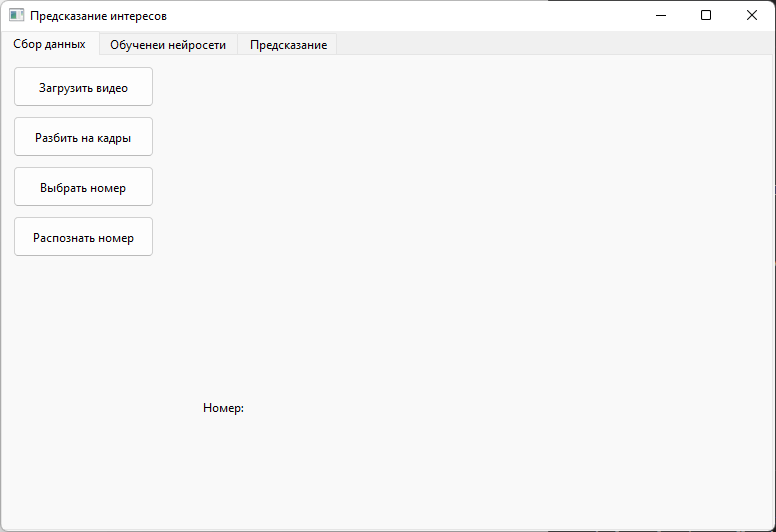
\includegraphics[width=0.5\textwidth]{window1}
	\caption{Окно программы}
	\label{f:window1}
\end{figure}

Выбор изображения представлен на рисунке~\ref{f:choose-pic}. Рядом с кнопками есть место для отрисовкм выбранного изображения.

\begin{figure}[h!]
	\centering
	\vspace{\toppaddingoffigure}
	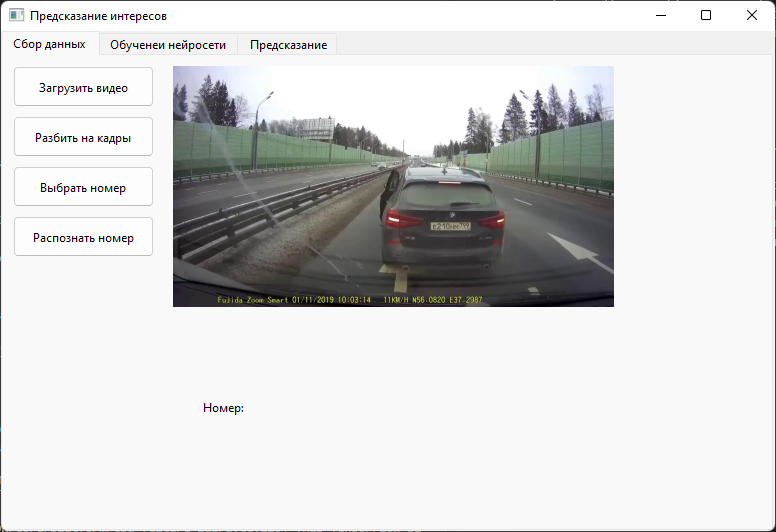
\includegraphics[width=0.5\textwidth]{choose-pic}
	\caption{Выбор изображения}
	\label{f:choose-pic}
\end{figure}

Распознавание номера представлено на рисунке~\ref{f:recognize}.

\begin{figure}[h!]
	\centering
	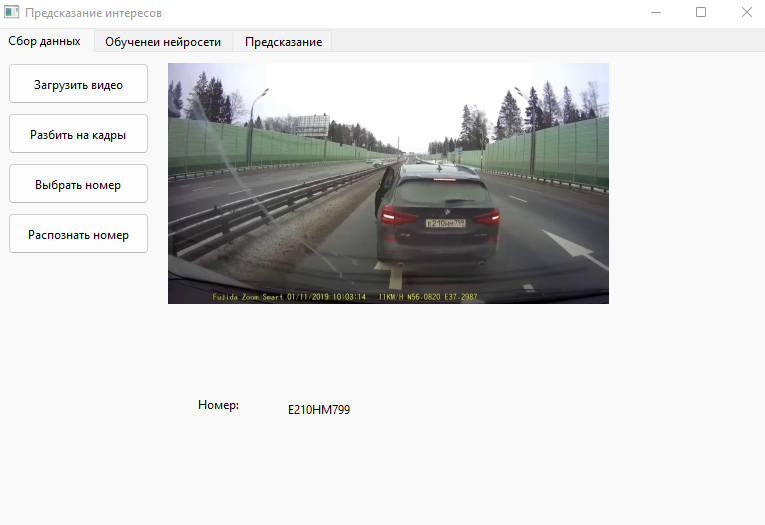
\includegraphics[width=0.5\textwidth]{recognize}
	\caption{Распознавание номера}
	\label{f:recognize}
\end{figure}


\newpage

Дальше происходит переход на сайт для определения модели автомобиля по распознанному номеру (рисунок~\ref{f:ident-model}).

\begin{figure}[h!]
	\centering
    \vspace{\toppaddingoffigure}
	
\includegraphics[width=0.5\textwidth]{ident-model}
	\caption{Определение модели авто}
	\label{f:ident-model}
\end{figure}


После этого предлагается выбрать изображение с бланком (рисунок~\ref{f:blank-examp}).

\begin{figure}[h!]
	\centering
	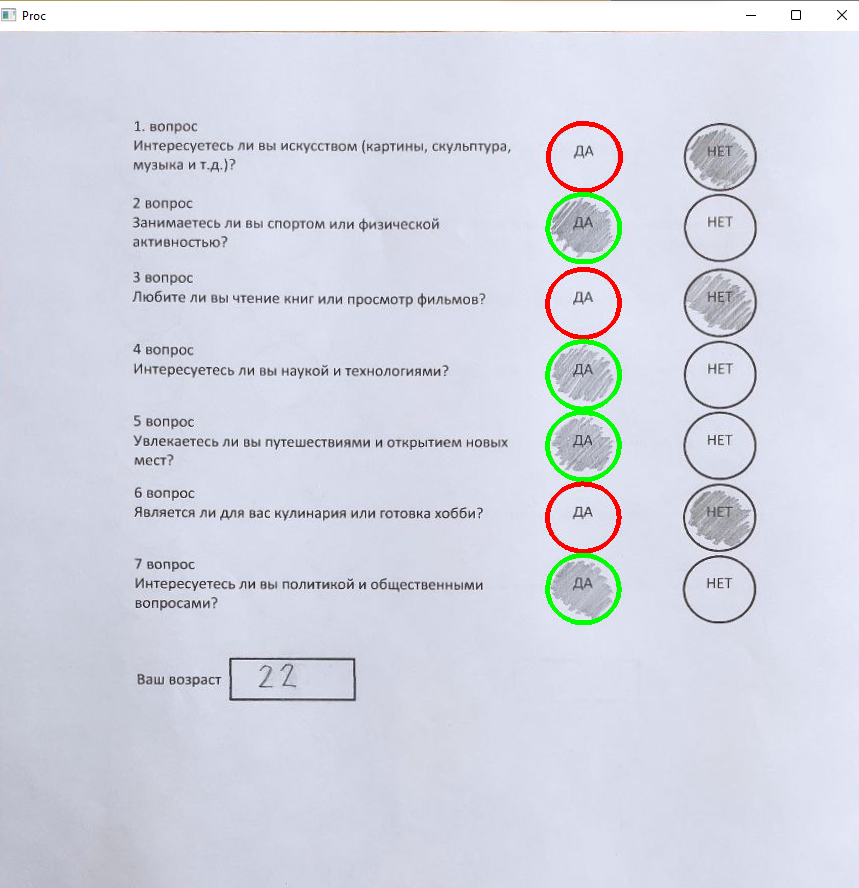
\includegraphics[width=0.5\textwidth]{blank-examp}
	\caption{Бланк опроса}
	\label{f:blank-examp}
\end{figure}


На бланке происходит обводка ответов. красным обводится в случае ответа НЕТ, а зеленым – в случае ответа ДА. Так же происходит считывание возраста, указанного в специальном поле.

Для удобства отладки происходит вывод в консоль (рисунок~\ref{f:console-log}).

\begin{figure}[h]
	\centering
	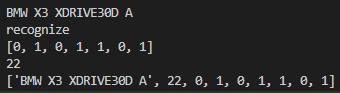
\includegraphics[width=0.5\textwidth]{console-log}
	\caption{Работа программы}
	\label{f:console-log}
\end{figure}

\newpage
Как можно увидеть по рисунку~\ref{f:console-log}, была определена модель автомобиля, так же выведен массив, содержащий ответы на вопросы. «0» означает ответ НЕТ, а «1» - ответ ДА. Кроме того, можно увидеть распознанный возраст «22». В конце все данные объединяются в единое целое, для записи в датасет – файл формата CSV. Результат записи представлен на рисунке~\ref{f:dataset}.

\begin{figure}[h!]
	\centering
    \vspace{\toppaddingoffigure}
	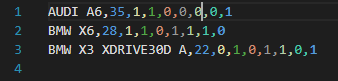
\includegraphics[width=0.5\textwidth]{dataset}
	\caption{Датасет}
	\label{f:dataset}
\end{figure}

\newpage
Окно для обучения нейросети представлено на рисунке~\ref{f:window2}. Имеются 2 кнопки дял выбора файла и начала обучения.

\begin{figure}[h!]
	\centering
    \vspace{\toppaddingoffigure}
	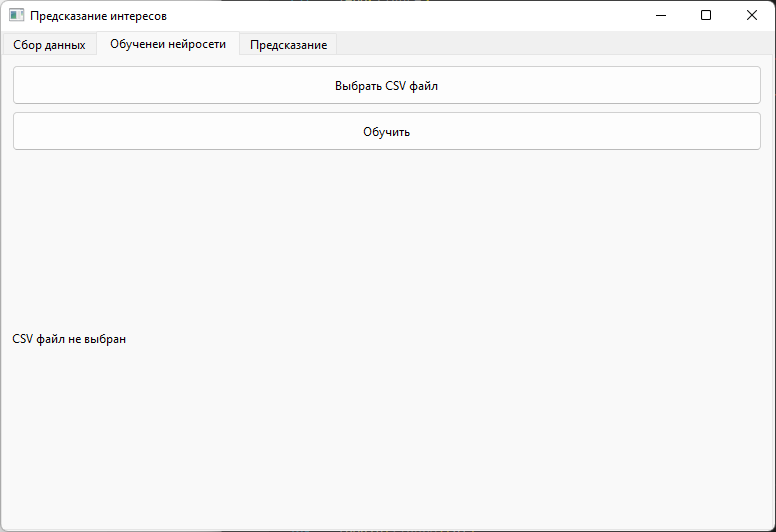
\includegraphics[width=0.5\textwidth]{window2}
	\caption{Окно программы}
	\label{f:window2}
\end{figure}

После выбора файла датасета выводится сообщение о выбранном файле (рисунок~\ref{f:window2.1}). Дальше можно приступать к обучению. По итогу обучения создается модель с расиширением ".keras".

\begin{figure}[h!]
	\centering
    \vspace{\toppaddingoffigure}
	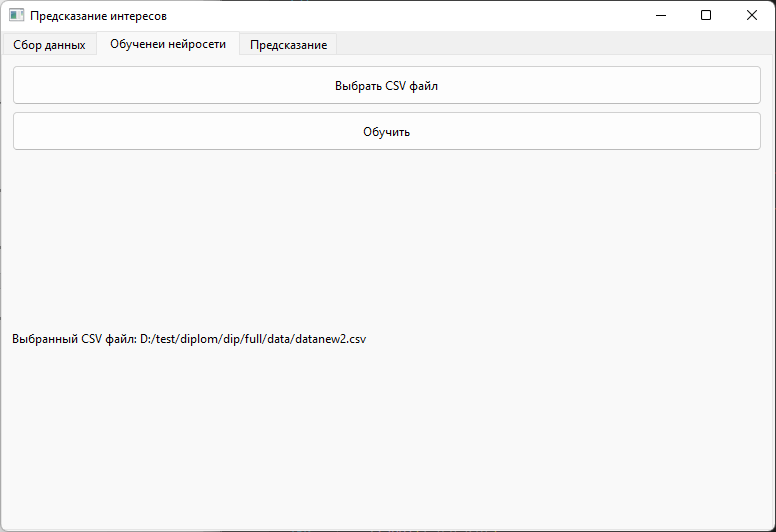
\includegraphics[width=0.5\textwidth]{window2.1}
	\caption{Окно программы}
	\label{f:window2.1}
\end{figure}

\newpage
Окно для предсказания интересов придставелно на рисунке~\ref{f:window3}.
\begin{figure}[h!]
	\centering
    \vspace{\toppaddingoffigure}
	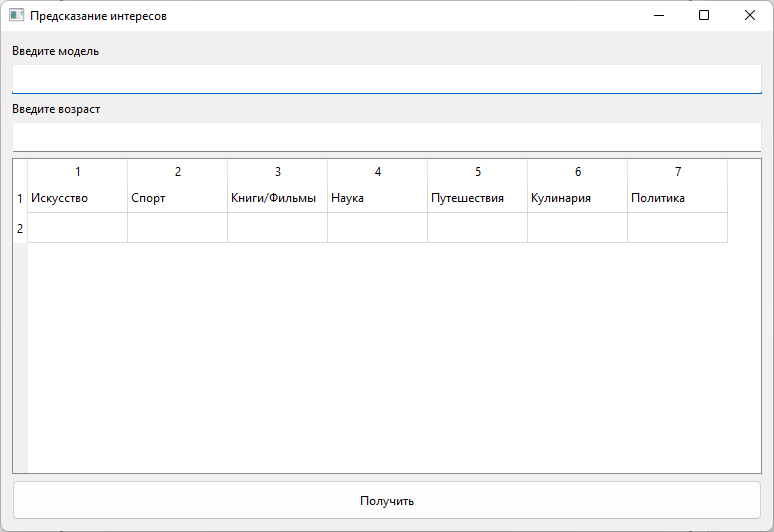
\includegraphics[width=0.5\textwidth]{window3}
	\caption{Окно программы}
	\label{f:window3}
\end{figure}

В поля для ввода необходимо ввести данные: название автомобиля и возраст владельца. После этого нажать на кнопку внизу экрана. Дальше модуль проведет работу, используя обученную модель для прогнозирования интересов. Результат работы представлен на рисунке~\ref{f:res-mod-pred}.
\begin{figure}[h!]
	\centering
    \vspace{\toppaddingoffigure}
	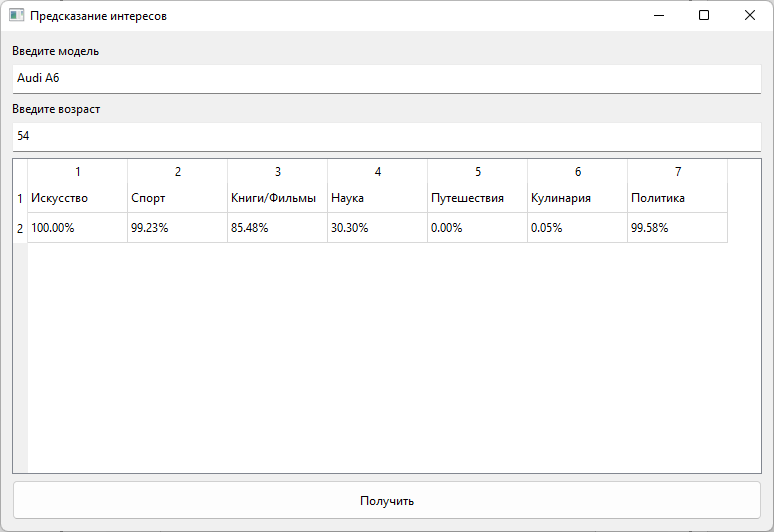
\includegraphics[width=0.5\textwidth]{res-mod-pred}
	\caption{Результат работы модуля}
	\label{f:res-mod-pred}
\end{figure}




\newpage
\section*{Выводы}
В двнном разделе были описаны основные технологии, которые использовались при разработке модулей, из которых состоит система. Было дано пояснение к основным функциям, а также расписан порядок их выполнения.
\newpage

\csection{Заключение}

В ходе выполнения проекта был разработан программная система, которая позволяет собирать информацию об интересах посетителей парковки и прогнозировать эти интересы. Для этого было использовано машинное обучение, методы компьютерного зрения и обработки опросных данных. 

Основной целью проекта было создать систему, которая поможет маркетологам анализировать интересы клиентов.

В процессе работы был проведен анализ предметной области, выявлены актуальность темы и ключевые требования. Были рассмотрены методы анализа данных, машинного обученияя и принцыпы копьютерного зрения.

Для реализации функционала были разработаны следующие компоненты: анализатор бланков, поиск модели автомобиля и распознавание номера. Кроме того были созданы скрипты для обучения нейронной сети с автоматизированным подбором гиперпараметров, а также для работы с обученной моделью. С помощью библиотеки-тюнера были подобраны наилучшие параметры для обучения и выбора оптимальной структуры нейронной сети.

Анализатор бланков позволяет автоматически обрабатывать изображения анкет, извлекать информацию об ответах на вопросы и возрасте. Для этого используются технологии обработки изображений и распознавания текста.

Компонент поиска модели автомобиля обеспечивает автоматизированный доступ к информации о моделях автомобилей. Для этого используется взаимодействие с сайтом, предоставляющим данные о транспортных средствах.

Компонент распознавания номера автомобиля служит для определения номера на изображении. Для этого используется предобученная модель машинного обучения.

В результате работы была разработана программная система, которая может быть использована в реальных задачах, направленных на анализ интересов посетителей парковок. Разработанная система принесет пользу для маркетологов и 
других людей, котороые работают с клиентами. Она помогает легко собирать и анализировать информацию о том, что нравится посетителям парковки. Это позволяет более точно нацеливать 
рекламные компании и предложения, что, в свою очередь, улучшает впечателния клиентов и делает маркетинг более эффективным.
% \newpage

\docappendix{Библиографический список}

\begin{references}
	\item\label{ref:num-methods} Бахвалов Н.С., Жидков Н.П., Кобельников Г.М.
	Численные методы [Текст] – 4-е изд. – М:. БИНОМ. Лаборатория
	знаний, 2006. – 636 с.: ил.
	\item Безрученко Б.П., Смирнов Д.А.
	Статистическое моделирование по временным рядам [Электронный ресурс]
	Cарат. отд-ние Ин-та радиотехники и электроники РАН.
	– Электрон. дан. – Саратов, 2000. – Режим доступа:
	http://www.masters.donntu.edu.ua/2012/fknt/dorosh/library/article4.pdf,
	свободный. - Загл. с экрана.
	\item Перельмутер А.В. Расчетные модели сооружений и возможность их анализа [Текст] / А.В. Перельмутер, В.И.
	Сливкер. Киев: Сталь, 2002. 600 с.
	\item NeuroShell 2 [Электронный ресурс] – Режим доступа: http://www.neuroproject.ru/aboutproduct.php, свободный. –
	Загл. с экрана.
	\item\label{ref:time-series-analysis} Бокс Дж., Дженкинс Г. Анализ временных рядов.
	Прогноз и управление [Текст]. - М.: Мир, 1974.

	\label{ref:total}
\end{references}

\docappendix{Авторская справка}\label{ax:authornote}
\begin{singlespace}

	\newcommand{\authorfullname}{Жеребцов Кирилл Андреевич}
	\renewcommand{\authorwithinitials}{Жеребцов К. А.}
	\renewcommand{\headofdepartment}{М. Л. Долженкова}

	Я, \authorfullname , автор выпускной квалификационной
	работы «\topic» сообщаю, что мне известно о персональной ответственности автора
	за разглашение сведений, подлежащих защите законами РФ о защите объектов
	интеллектуальной собственности.

	Одновременно сообщаю, что:

	1. При подготовке к защите выпускной квалификационной работы не
	использованы источники (документы, отчёты, диссертации, литература и т.п.),
	имеющие гриф секретности или «Для служебного пользования» ФГБОУ ВО
	«Вятский государственный университет» или другой организации.

	2. Данная работа не связана с незавершёнными исследованиями или уже
	с завершёнными, но ещё официально не разрешёнными к опубликованию
	ФГБОУ ВО «Вятский государственный университет» или другими
	организациями.

	3. Данная работа не содержит коммерческую информацию, способную
	нанести ущерб интеллектуальной собственности ФГБОУ ВО «Вятский
	государственный университет» или другой организации.

	4. Данная работа не является результатом НИР или ОКР, выполняемой по
	договору с организацией.

	5. В предлагаемом к опубликованию тексте нет данных по
	незащищённым объектам интеллектуальной собственности других авторов.

	6. Использование моей дипломной работы в научных исследованиях
	оформляется в соответствии с законодательством РФ о защите интеллектуальной
	собственности отдельным договором.

	\newcommand{\daysize}{2em}

	\newcommand{\confirm}{
		\noindent
		Сведения по авторской справке подтверждаю:~«\uline{\hspace{\daysize}}»
	}

	\newcommand{\verticalspacesize}{2em}

	\newcommand{\rightindent}{2em}

	\newcommand{\customtheyear}{\the\year~г.}

	\newcommand{\rightindentwithyear}{\widthof{\customtheyear}+\rightindent}

	\newcommand{\signaturesize}{6.6em}

	\vspace{\verticalspacesize}


	\noindent
	Автор: \authorwithinitials~«\uline{\hspace{\daysize}}»
	\uline{\hspace{6em}}
	\customtheyear
	\hfill
	\uline{\hspace{\signaturesize}}\hspace{\rightindentwithyear}

	\vspace{-0.3em}
	\hfill
	\makebox[\signaturesize][c]{\small подпись}
	\hspace{\rightindentwithyear}

	\vspace{\verticalspacesize}

	\confirm
	\uline{\hfill}\customtheyear\hspace{\rightindent}

	\vspace{\verticalspacesize}

	\noindent
	Заведующий кафедрой ЭВМ: \headofdepartment
	\hfill
	\uline{\hspace{\signaturesize}}\hspace{\rightindentwithyear}

	\vspace{-0.3em}
	\hfill
	\makebox[\signaturesize][c]{\small подпись}
	\hspace{\rightindentwithyear}

\end{singlespace}




\docappendix{Листинг кода}\label{ax:code}

\begin{lstlisting}
    # Component for searching car models using the autoteka.ru website 
    from selenium import webdriver
    from selenium.webdriver.common.keys import Keys
    from selenium.webdriver.common.by import By
    from selenium.webdriver.support.ui import WebDriverWait  # Импортируем WebDriverWait
    from selenium.webdriver.support import expected_conditions as EC
    import time

    # Path to driver
    driver_path = 'drv/chromedriver-win64/chromedriver.exe'

    # URL link to the page
    website_url = 'https://autoteka.ru/'

    # Initializing the driver
    chrome_service = webdriver.chrome.service.Service(driver_path)
    driver = webdriver.Chrome(service=chrome_service)

    # Function for parsing
    def site(number):
        input = number
        driver.get(website_url)

        input_field = driver.find_element(By.NAME, 'identifier')
        input_field.send_keys(input)
        input_field.send_keys(Keys.ENTER)

        WebDriverWait(driver, 15).until(EC.url_changes(website_url))

        time.sleep(5)

        text_element = driver.find_element(By.CLASS_NAME, 'pit4K')
        text = text_element.text

        time.sleep(3)

        lines = text.split('\n')
        result = ' '.join(lines[:2])

        driver.quit()

        return result.split(',')[0].strip()
\end{lstlisting}

\begin{lstlisting}
    # Component for analyzing forms
    from imutils.perspective import four_point_transform
    from imutils import contours
    import numpy as np
    import argparse
    import imutils
    import cv2
    import csv
    import re
    import pytesseract
    
    # Define the correct answers for the exam (placeholder)
    ANSWER_KEY = {0: 0, 1: 0, 2: 0, 3: 0, 4: 0, 5: 0, 6: 0}
    
    # Path to Tesseract executable
    pytesseract.pytesseract.tesseract_cmd = r'C:\\Program Files\\Tesseract-OCR\\tesseract.exe'
    
    # Tesseract OCR configuration
    custom_config = r'--oem 3 --psm 6'
    
    def process_exam(image_path):
        # Read the input image
        image = cv2.imread(image_path)
        
        # Convert the image to grayscale
        gray = cv2.cvtColor(image, cv2.COLOR_BGR2GRAY)
        
        # Apply GaussianBlur to reduce noise and detail in the image
        blurred = cv2.GaussianBlur(gray, (5, 5), 0)
        
        # Use Canny edge detector to find edges in the image
        edged = cv2.Canny(blurred, 75, 200)
    
        # Find contours in the edged image
        cnts = cv2.findContours(edged.copy(), cv2.RETR_EXTERNAL, cv2.CHAIN_APPROX_SIMPLE)
        cnts = imutils.grab_contours(cnts)
        docCnt = None
    
        # Ensure at least one contour was found
        if len(cnts) > 0:
            # Sort the contours by area, keeping only the largest one
            cnts = sorted(cnts, key=cv2.contourArea, reverse=True)
            for c in cnts:
                # Approximate the contour
                peri = cv2.arcLength(c, True)
                approx = cv2.approxPolyDP(c, 0.02 * peri, True)
                
                # If the approximated contour has four points, assume it's the paper
                if len(approx) == 4:
                    docCnt = approx
                    break
    
        # Apply a perspective transform to obtain a top-down view of the paper
        paper = four_point_transform(image, docCnt.reshape(4, 2))
        warped = four_point_transform(gray, docCnt.reshape(4, 2))
    
        # Apply a binary threshold to the warped image
        thresh = cv2.threshold(warped, 0, 255, cv2.THRESH_BINARY_INV | cv2.THRESH_OTSU)[1]
    
        # Find contours in the thresholded image
        cnts = cv2.findContours(thresh.copy(), cv2.RETR_EXTERNAL, cv2.CHAIN_APPROX_SIMPLE)
        cnts = imutils.grab_contours(cnts)
        questionCnts = []
    
        # Loop over the contours
        for c in cnts:
            (x, y, w, h) = cv2.boundingRect(c)
            ar = w / float(h)
            
            # Filter the contours to find those that correspond to question bubbles
            if (w >= 50) and (h >= 50) and (ar >= 0.9) and (ar <= 1.1):
                questionCnts.append(c)
    
        # Sort the question contours top-to-bottom
        questionCnts = contours.sort_contours(questionCnts, method="top-to-bottom")[0]
        results = []
    
        # Loop over the question groups
        for (q, i) in enumerate(np.arange(0, len(questionCnts), 2)):
            cnts = contours.sort_contours(questionCnts[i:i + 2])[0]
            bubbled = None
            question_result = 0
    
            # Loop over the sorted contours
            for (j, c) in enumerate(cnts):
                mask = np.zeros(thresh.shape, dtype="uint8")
                cv2.drawContours(mask, [c], -1, 255, -1)
    
                mask = cv2.bitwise_and(thresh, thresh, mask=mask)
                total = cv2.countNonZero(mask)
                if bubbled is None or total > bubbled[0]:
                    bubbled = (total, j)
    
            color = (0, 0, 255)
            k = ANSWER_KEY[q]
    
            if k == bubbled[1]:
                question_result = 1
                color = (0, 255, 0)
    
            cv2.drawContours(paper, [cnts[k]], -1, color, 3)
            results.append(question_result)
    
        print(results)
    
        cv2.imshow("Proc", paper)
        cv2.waitKey(0)
    
        return results
    
    def get_age(image_path):
        # Read the input image
        image = cv2.imread(image_path)
        
        # Convert the image to grayscale
        gray = cv2.cvtColor(image, cv2.COLOR_BGR2GRAY)
        
        # Apply GaussianBlur to reduce noise and detail in the image
        blurred = cv2.GaussianBlur(gray, (5, 5), 0)
        
        # Use Canny edge detector to find edges in the image
        edged = cv2.Canny(blurred, 75, 200)
    
        # Find contours in the edged image
        cnts = cv2.findContours(edged.copy(), cv2.RETR_EXTERNAL, cv2.CHAIN_APPROX_SIMPLE)
        cnts = imutils.grab_contours(cnts)
        docCnt = None
    
        # Ensure at least one contour was found
        if len(cnts) > 0:
            # Sort the contours by area, keeping only the largest one
            cnts = sorted(cnts, key=cv2.contourArea, reverse=True)
            for c in cnts:
                # Approximate the contour
                peri = cv2.arcLength(c, True)
                approx = cv2.approxPolyDP(c, 0.02 * peri, True)
                
                # If the approximated contour has four points, assume it's the paper
                if len(approx) == 4:
                    docCnt = approx
                    break
    
        # Apply a perspective transform to obtain a top-down view of the paper
        paper = four_point_transform(image, docCnt.reshape(4, 2))
    
        # Further process the transformed image to find the age
        gray = cv2.cvtColor(paper, cv2.COLOR_BGR2GRAY)
        blurred = cv2.GaussianBlur(gray, (5, 5), 0)
        edged = cv2.Canny(blurred, 75, 200)
    
        cnts = cv2.findContours(edged.copy(), cv2.RETR_EXTERNAL, cv2.CHAIN_APPROX_SIMPLE)
        cnts = imutils.grab_contours(cnts)
        docCnt = None
    
        if len(cnts) > 0:
            cnts = sorted(cnts, key=cv2.contourArea, reverse=True)
            for c in cnts:
                peri = cv2.arcLength(c, True)
                approx = cv2.approxPolyDP(c, 0.02 * peri, True)
                if len(approx) == 4:
                    docCnt = approx
                    break
    
        paper = four_point_transform(paper, docCnt.reshape(4, 2))
    
        gray = cv2.cvtColor(paper, cv2.COLOR_BGR2GRAY)
        thresh = cv2.threshold(gray, 0, 255, cv2.THRESH_BINARY_INV | cv2.THRESH_OTSU)[1]
        
        # Use OCR to extract text from the thresholded image
        text = pytesseract.image_to_string(thresh, config=custom_config)
        
        # Find all two-digit numbers in the extracted text
        number = re.findall(r'\b\d+\b', text)
        two_digit_numbers = ' '.join(num for num in number if len(num) == 2)
        print(two_digit_numbers)
        return two_digit_numbers
    
    def write_to_csv(filename, results):
        # Append the results to a CSV file
        with open(filename, mode='a', newline='') as file:
            writer = csv.writer(file)
            writer.writerow(results)
    
    def blank(path_in, path_out, model):
        print(path_in)
        print(path_out)
        
        # Process the exam and get the age
        results = process_exam(path_in)
        age = get_age(path_in)
        
        # Insert model and age to the results
        results.insert(0, int(age))
        results.insert(0, model)
        
        print(results)
        write_to_csv(path_out, results)
        print("done")
    
    def main():
        # Set up argument parser
        ap = argparse.ArgumentParser()
        ap.add_argument("-i", "--image", required=True, help="path to the input image")
        ap.add_argument("-o", "--output", required=True, help="path to save the output CSV file")
        args = vars(ap.parse_args())
        
        # Process the exam and get the age
        results = process_exam(args["image"])
        age = get_age(args["image"])
        
        # Insert age to the results
        results.insert(0, int(age))
        print(results)
        
        # Write results to the CSV file
        write_to_csv(args["output"], results)
    
    if __name__ == "__main__":
        main()    
\end{lstlisting}

\begin{lstlisting}
    # Component for working with a trained model
    import numpy as np
    import pandas as pd
    import tensorflow as tf
    from sklearn.preprocessing import OneHotEncoder
    import os

    # Transforming new data
    def preprocess_new_data(new_data, full_data):
        # Convert categorical column "Model" to numeric values ​​using OneHotEncoding
        encoder = OneHotEncoder()
        encoder.fit(full_data[['Model']])
        model_encoded = encoder.transform(new_data[['Model']]).toarray()
        
        # Normalization of numerical data (age)
        age = new_data[['Age']].values
        age_normalized = (age - np.mean(full_data['Age'])) / np.std(full_data['Age'])

        # Merging the transformed data
        X_new = np.concatenate([age_normalized, model_encoded], axis=1)
        
        return X_new

    # Receiving Predictions
    def get_predictions(X_new, model_p):
        predictions = model_p.predict(X_new)
        # binary_predictions = np.round(predictions)
        return predictions

    # Output results
    def print_results(binary_predictions):
        # print("New data:")
        # print(new_data)
        print("\nPredictions:")
        np.set_printoptions(threshold=np.inf)
        print(binary_predictions)

    def main(model, age, model_pred):
        
        # Example of new data for testing
        new_data = pd.DataFrame({'Model': [model], 'Age': [int(age)]})

        # Transforming new data
        X_new = preprocess_new_data(new_data, full_data)

        if not os.path.isfile(model_pred):
            raise FileNotFoundError(f"Файл {model_pred} не найден")

        # Check file extension
        if not model_pred.endswith('.keras'):
            raise ValueError("Неправильный формат файла. Ожидался файл с расширением .keras")

        model_p = tf.keras.models.load_model(model_pred)

        # Getting predictions for just one example
        binary_predictions = get_predictions(X_new, model_p)

        art_prediction = binary_predictions[0][0]
        sport_prediction = binary_predictions[0][1]
        book_films_prediction = binary_predictions[0][2]
        science_prediction = binary_predictions[0][3]
        travel_prediction = binary_predictions[0][4]
        cooking_prediction = binary_predictions[0][5]
        politics_prediction = binary_predictions[0][6]

        # Writing to an array
        predictions_array = [art_prediction, sport_prediction, book_films_prediction, science_prediction, travel_prediction, cooking_prediction, politics_prediction]

        return predictions_array
\end{lstlisting}

\begin{lstlisting}
    # Component for training neural networks
    import pandas as pd
    import numpy as np
    import tensorflow as tf
    from tensorflow import keras
    from sklearn.model_selection import train_test_split, GridSearchCV
    from sklearn.preprocessing import OneHotEncoder
    from scikeras.wrappers import KerasClassifier
    from tensorflow.python.keras.callbacks import EarlyStopping, ModelCheckpoint
    from tqdm.keras import TqdmCallback

    # Load the dataset
    data = pd.read_csv('datanew2.csv')

    # Convert the categorical "Model" column to numerical values using OneHotEncoder
    encoder = OneHotEncoder()
    model_encoded = encoder.fit_transform(data[['Model']]).toarray()

    # Normalize the numerical "Age" column
    age = data[['Age']].values
    age_normalized = (age - np.mean(age)) / np.std(age)

    # Combine the normalized age data and the encoded model data
    X = np.concatenate([age_normalized, model_encoded], axis=1)

    # Extract the target variables (interests)
    y = data[['Art', 'Sport', 'Book/Films', 'Science', 'Travel', 'Cooking', 'Politics']].values

    # Split the data into training and test sets
    X_train, X_test, y_train, y_test = train_test_split(X, y, test_size=0.2, random_state=42)

    # Function to create the model with specified parameters
    def create_model(optimizer='adam', num_hidden_layers=2, num_neurons=20, activation='relu', dropout_rate=0.2, learning_rate=0.001):
        # Input layer
        inputs = tf.keras.Input(shape=(X.shape[1],))
        
        # First hidden layer
        x = tf.keras.layers.Dense(num_neurons, activation=activation)(inputs)
        x = tf.keras.layers.Dropout(dropout_rate)(x)
        
        # Additional hidden layers based on the parameter num_hidden_layers
        for _ in range(num_hidden_layers - 1):
            x = tf.keras.layers.Dense(num_neurons, activation=activation)(x)
            x = tf.keras.layers.Dropout(dropout_rate)(x)
        
        # Output layer with sigmoid activation for multi-label classification
        outputs = tf.keras.layers.Dense(7, activation='sigmoid')(x)
        
        # Create the model
        model = tf.keras.Model(inputs=inputs, outputs=outputs)
        
        # Set the optimizer based on the specified parameter
        if optimizer == 'adam':
            optimizer = tf.keras.optimizers.Adam(learning_rate=learning_rate)
        elif optimizer == 'rmsprop':
            optimizer = tf.keras.optimizers.RMSprop(learning_rate=learning_rate)
        elif optimizer == 'sgd':
            optimizer = tf.keras.optimizers.SGD(learning_rate=learning_rate)
        
        # Compile the model
        model.compile(optimizer=optimizer, loss='binary_crossentropy', metrics=['accuracy'])
        return model

    # Create a KerasClassifier with the create_model function
    model = KerasClassifier(model=create_model, verbose=0, epochs=100)

    # Define the grid of parameters for GridSearchCV
    param_grid = {
        'model__num_hidden_layers': [2, 3, 4, 5],
        'model__num_neurons': [20, 30, 40],
        'model__activation': ['relu', 'tanh'],
        'model__dropout_rate': [0.1, 0.2],
        'model__optimizer': ['adam', 'rmsprop', 'sgd'],
        'model__learning_rate': [0.001, 0.01, 0.1]
    }

    # Create a GridSearchCV object
    grid_search = GridSearchCV(estimator=model, param_grid=param_grid, cv=3, verbose=1, n_jobs=-1)

    # Fit the GridSearchCV object to the training data
    grid_search.fit(X_train, y_train)

    # Print the best parameters found by GridSearchCV
    print("Best: %f using %s" % (grid_search.best_score_, grid_search.best_params_))

    # Get the best parameters and create a model with them
    best_params = grid_search.best_params_
    best_model = create_model(
        optimizer=best_params['model__optimizer'],
        num_hidden_layers=best_params['model__num_hidden_layers'],
        num_neurons=best_params['model__num_neurons'],
        activation=best_params['model__activation'],
        dropout_rate=best_params['model__dropout_rate'],
        learning_rate=best_params['model__learning_rate']
    )

    # Define callbacks for early stopping, model checkpointing, and TQDM progress bar
    early_stopping = EarlyStopping(monitor='val_loss', patience=5, restore_best_weights=True)
    model_checkpoint = ModelCheckpoint('model.keras', save_best_only=True, monitor='val_loss', mode='min')
    tqdm_callback = TqdmCallback(verbose=1)

    # Train the best model with the callbacks
    history = best_model.fit(
        X_train, y_train,
        validation_split=0.2,
        epochs=100,
        callbacks=[early_stopping, model_checkpoint, tqdm_callback],
        verbose=0
    )

    # Evaluate the model on the test set
    loss, accuracy = best_model.evaluate(X_test, y_test)
    print(f'Test Accuracy: {accuracy}')
\end{lstlisting}

\begin{lstlisting}
    # Vehicle Number Plate Recognition Component
    import os
    from datetime import timedelta
    from pathlib import Path
    import matplotlib.pyplot as plt
    import cv2
    import numpy as np
    import re
    import imutils
    import pytesseract
    import pytesseract as tess
    tess.pytesseract.tesseract_cmd = r'Tesseract-OCR\tesseract.exe'
    from PyQt6 import uic
    from PyQt6.QtGui import QPixmap
    from PyQt6.QtWidgets import QApplication, QFileDialog, QMessageBox
    from imutils import contours
    from moviepy.editor import VideoFileClip
    import json
    import sqlite3
    import itertools
    import tensorflow as tf
    from skimage.feature import canny
    from skimage.transform import hough_line, hough_line_peaks, rotate
    from skimage.color import rgb2gray

    import matplotlib.gridspec as gridspec
    import cv2

    import autoteka
    import test_blank

    # Constants for saving frames per second from video
    SAVING_FRAMES_PER_SECOND = 1

    # Load the UI design file
    Form, Window = uic.loadUiType("Parking.ui")

    # Initialize the application and load the UI window
    app = QApplication([])
    window = Window()
    form = Form()
    form.setupUi(window)
    window.show()

    # Global variables to store the paths of video, image, and the result
    video_file = ''
    image_file = ''
    result = ''
    arr = []

    # Function to format the time delta for naming frames
    def format_timedelta(td):
        result = str(td)
        try:
            result, ms = result.split(".")
        except ValueError:
            return result + ".00".replace(":", "-")

        ms = round(int(ms) / 10000)
        return f"{result}.{ms:02}".replace(":", "-")

    # Function to load the video file
    def load():
        global video_file
        video_file = QFileDialog.getOpenFileName()
        path = Path(video_file[0])
        video_file = path.name
        print("load")

    # Function to split the video into frames
    def split():
        video_clip = VideoFileClip(video_file)
        filename, _ = os.path.splitext(video_file)

        if not os.path.isdir(filename):
            os.mkdir(filename)

        saving_frames_per_second = min(video_clip.fps, SAVING_FRAMES_PER_SECOND)
        step = 1 / video_clip.fps if saving_frames_per_second == 0 else 1 / saving_frames_per_second

        for current_duration in np.arange(0, video_clip.duration, step):
            frame_duration_formatted = format_timedelta(timedelta(seconds=current_duration)).replace(":", "-")
            frame_filename = os.path.join(filename, f"frame{frame_duration_formatted}.jpg")

            video_clip.save_frame(frame_filename, current_duration)
        print("split")

    # Function to check the format of the recognized license plate
    def check_format(variable):
        pattern = r'^[A-Z]\d{3}[A-Z]{2}\d{3}$'
        pattern2 = r'^[A-Z]\d{3}[A-Z]{2}\d{2}$'
        if re.match(pattern, variable) or re.match(pattern2, variable):
            return True
        else:
            return False

    # Function to choose an image file for recognition
    def choose():
        global image_file
        image_file = QFileDialog.getOpenFileName()
        image_file = image_file[0]
        form.label_6.setPixmap(QPixmap(image_file))
        form.label_6.setScaledContents(True)
        print("choose")

    # Function to recognize text from the car plate
    def carplate_text():
        global image_file

        image0 = cv2.imread(image_file)
        image_height, image_width, _ = image0.shape
        image = cv2.resize(image0, (1024, 1024))
        image = image.astype(np.float32)
        paths = 'model/recognize/model_resnet.tflite'
        interpreter = tf.lite.Interpreter(model_path=paths)
        interpreter.allocate_tensors()
        input_details = interpreter.get_input_details()
        output_details = interpreter.get_output_details()
        X_data1 = np.float32(image.reshape(1, 1024, 1024, 3))

        interpreter.set_tensor(input_details[0]['index'], X_data1)
        interpreter.invoke()
        detection = interpreter.get_tensor(output_details[0]['index'])
        net_out_value2 = interpreter.get_tensor(output_details[1]['index'])
        net_out_value3 = interpreter.get_tensor(output_details[2]['index'])
        net_out_value4 = interpreter.get_tensor(output_details[3]['index'])

        img = image0
        razmer = img.shape

        img2 = cv2.cvtColor(img, cv2.COLOR_BGR2RGB)
        img3 = img[:, :, :]

        number = 0
        while number < len(detection[0][number]) and detection[0, number, 0] > 0.9:
            number = number + 1

        box_x = int(detection[0, number, 0] * image_height)
        box_y = int(detection[0, number, 1] * image_width)
        box_width = int(detection[0, number, 2] * image_height)
        box_height = int(detection[0, number, 3] * image_width)

        cv2.rectangle(img2, (box_y, box_x), (box_height, box_width), (230, 230, 21), thickness=5)

        net_out_value3

        image = image0[box_x:box_width, box_y:box_height, :]
        img2 = cv2.cvtColor(image, cv2.COLOR_BGR2RGB)

        grayscale = rgb2gray(image)
        edges = canny(grayscale, sigma=3.0)
        out, angles, distances = hough_line(edges)
        h, theta, d = out, angles, distances
        angle_step = 0.5 * np.diff(theta).mean()
        d_step = 0.5 * np.diff(d).mean()
        bounds = [np.rad2deg(theta[0] - angle_step),
                np.rad2deg(theta[-1] + angle_step),
                d[-1] + d_step, d[0] - d_step]

        _, angles_peaks, _ = hough_line_peaks(out, angles, distances, num_peaks=20)
        angle = np.mean(np.rad2deg(angles_peaks))

        if 0 <= angle <= 90:
            rot_angle = angle - 90
        elif -45 <= angle < 0:
            rot_angle = angle - 90
        elif -90 <= angle < -45:
            rot_angle = 90 + angle
        if abs(rot_angle) > 20:
            rot_angle = 0

        rotated = rotate(image, rot_angle, resize=True) * 255
        rotated = rotated

        rotated1 = rotated[:, :, :]
        if rotated.shape[1] / rotated.shape[0] < 2:
            minus = np.abs(int(np.sin(np.radians(rot_angle)) * rotated.shape[0]))
            rotated1 = rotated[minus:-minus, :, :]
            print(minus)

        lab = cv2.cvtColor(rotated1, cv2.COLOR_BGR2LAB)
        l, a, b = cv2.split(lab)
        clahe = cv2.createCLAHE(clipLimit=3.0, tileGridSize=(8, 8))
        cl = clahe.apply(l)
        limg = cv2.merge((cl, a, b))
        final = cv2.cvtColor(limg, cv2.COLOR_LAB2BGR)

        letters = ['0', '1', '2', '3', '4', '5', '6', '7', '8', '9', 'A', 'B', 'C', 'E', 'H', 'K', 'M', 'O', 'P', 'T', 'X',
                'Y']

        def decode_batch(out):
            ret = []
            for j in range(out.shape[0]):
                out_best = list(np.argmax(out[j, 2:], 1))
                out_best = [k for k, g in itertools.groupby(out_best)]
                outstr = ''
                for c in out_best:
                    if c < len(letters):
                        outstr += letters[c]
                ret.append(outstr)
            return ret

        paths = 'model/recognize/model1_nomer.tflite'
        interpreter = tf.lite.Interpreter(model_path=paths)
        interpreter.allocate_tensors()

        input_details = interpreter.get_input_details()
        output_details = interpreter.get_output_details()
        img = final
        img = cv2.cvtColor(img, cv2.COLOR_BGR2GRAY)
        img = cv2.resize(img, (128, 64))
        img = img.astype(np.float32)
        img /= 255

        img1 = img.T
        img1.shape
        X_data1 = np.float32(img1.reshape(1, 128, 64, 1))
        input_index = (interpreter.get_input_details()[0]['index'])
        interpreter.set_tensor(input_details[0]['index'], X_data1)

        interpreter.invoke()

        net_out_value = interpreter.get_tensor(output_details[0]['index'])
        pred_texts = decode_batch(net_out_value)
        pred_texts

        fig = plt.figure(figsize=(10, 10))
        outer = gridspec.GridSpec(2, 1, wspace=10, hspace=0.1)
        ax1 = plt.Subplot(fig, outer[0])
        fig.add_subplot(ax1)
        ax2 = plt.Subplot(fig, outer[1])
        fig.add_subplot(ax2)
        return pred_texts[0]

    # Function to recognize the license plate and display information
    def recognize():
        global result
        result = carplate_text().upper()
        print(result)
        if result == '':
            QMessageBox.information(None, "Ошибка распознания", "НЕ РАСПОЗНАНО")
        elif check_format(result) != True:
            QMessageBox.information(None, "Ошибка формата", "Результат:" + result)
        else:
            form.label_7.setText(result)

            count = 0
            for i in range(len(arr)):
                if arr[i][0] == result:
                    count += 1

            if count == 0:
                arr.append([result, 1])
            else:
                for i in range(len(arr)):
                    if arr[i][0] == result:
                        arr[i][1] += 1

            for i in range(len(arr)):
                if arr[i][0] == result:
                    form.label_2.setText(str(arr[i][1]))
                    if arr[i][1] < 5:
                        form.label_5.setText('0%')
                    elif 5 <= arr[i][1] < 10:
                        form.label_5.setText('5%')
                    elif 10 <= arr[i][1] < 20:
                        form.label_5.setText('10%')
                    else:
                        form.label_5.setText('15%')
        
        model = autoteka.site(result)
        print(model)
        print("recognize")

        file_path, _ = QFileDialog.getOpenFileName()
        test_blank.blank(file_path, 'data/data.csv', model)

    # Connect UI buttons to their respective functions
    form.pushButton.clicked.connect(load)
    form.pushButton_2.clicked.connect(split)
    form.pushButton_3.clicked.connect(choose)
    form.pushButton_4.clicked.connect(recognize)

    # Start the application event loop
    app.exec()
\end{lstlisting}

\begin{lstlisting}
    #Interface
    # Importing necessary modules and libraries
    from PyQt6.QtWidgets import (
        QApplication, 
        QWidget, 
        QPushButton, 
        QLabel, 
        QVBoxLayout, 
        QTextEdit, 
        QTableWidget, 
        QTableWidgetItem,
        QTabWidget,
        QMainWindow,
        QFileDialog,
        QMessageBox
    )
    from PyQt6 import QtCore

    # Constant for saving frames per second from a video
    SAVING_FRAMES_PER_SECOND = 1

    # List of interest categories
    list_int = ["Искусство", "Спорт", "Книги/Фильмы", "Наука", "Путешествия", "Кулинария", "Политика"]

    # Global variables for storing file paths and results
    video_file = ''
    image_file = ''
    result = ''
    arr = []

    # Main window class inheriting from QMainWindow
    class MainWindow(QMainWindow):
        def __init__(self):
            super().__init__()

            self.setWindowTitle("Предсказание интересов")
            self.setGeometry(400, 250, 750, 500)

            # Creating a tab widget and setting it as the central widget
            self.tabs = QTabWidget()
            self.setCentralWidget(self.tabs)

            # Creating tabs
            self.create_tabs()

            self.model_pred = ""

        # Method to create tabs
        def create_tabs(self):
            # Creating the first tab for data collection
            tab1 = QWidget()
            
            self.pushButton = QPushButton(tab1)
            self.pushButton.setGeometry(QtCore.QRect(10, 10, 141, 41))
            self.pushButton.setObjectName("pushButton")
            self.pushButton.clicked.connect(self.load)
            self.pushButton.setText("Загрузить видео")

            self.pushButton_2 = QPushButton(tab1)
            self.pushButton_2.setGeometry(QtCore.QRect(10, 60, 141, 41))
            self.pushButton_2.setObjectName("pushButton_2")
            self.pushButton_2.clicked.connect(self.split)
            self.pushButton_2.setText("Разбить на кадры")

            self.pushButton_3 = QPushButton(tab1)
            self.pushButton_3.setGeometry(QtCore.QRect(10, 110, 141, 41))
            self.pushButton_3.setObjectName("pushButton_3")
            self.pushButton_3.clicked.connect(self.choose)
            self.pushButton_3.setText("Выбрать номер")

            self.pushButton_4 = QPushButton(tab1)
            self.pushButton_4.setGeometry(QtCore.QRect(10, 160, 141, 41))
            self.pushButton_4.setObjectName("pushButton_4")
            self.pushButton_4.clicked.connect(self.recognize)
            self.pushButton_4.setText("Распознать номер")

            self.label_6 = QLabel(tab1)
            self.label_6.setGeometry(QtCore.QRect(170, 10, 441, 241))
            self.label_6.setText("")
            self.label_6.setAlignment(QtCore.Qt.AlignmentFlag.AlignCenter)
            self.label_6.setObjectName("label_6")

            self.label_3 = QLabel(tab1)
            self.label_3.setGeometry(QtCore.QRect(200, 340, 71, 21))
            self.label_3.setText("Номер:")
            self.label_3.setObjectName("label_3")

            self.label_7 = QLabel(tab1)
            self.label_7.setGeometry(QtCore.QRect(290, 340, 161, 31))
            self.label_7.setText("")
            self.label_7.setObjectName("label_7")

            # Creating the second tab for neural network training
            tab2 = QWidget()
            tab2_layout = QVBoxLayout()

            self.pushButton_csv = QPushButton(tab2)
            self.pushButton_csv.setText("Выбрать CSV файл")
            self.pushButton_csv.setFixedSize(750, 40)
            self.pushButton_csv.clicked.connect(self.choose_csv_file)
            tab2_layout.addWidget(self.pushButton_csv)

            self.pushButton_learn = QPushButton(tab2)
            self.pushButton_learn.setText("Обучить")
            self.pushButton_learn.setFixedSize(750, 40)
            self.pushButton_learn.clicked.connect(self.learn)
            tab2_layout.addWidget(self.pushButton_learn)

            self.label_csv = QLabel(tab2)
            self.label_csv.setText("CSV файл не выбран")
            tab2_layout.addWidget(self.label_csv)

            tab2.setLayout(tab2_layout)

            # Creating the third tab for prediction
            tab3 = QWidget()
            tab3_layout = QVBoxLayout()

            self.label_model = QLabel('Введите модель', tab3)
            self.label_age = QLabel('Введите возраст', tab3)

            self.text_edit_model = QTextEdit(tab3)
            self.text_edit_model.setFixedSize(750, 30)
            
            self.text_edit_age = QTextEdit(tab3)
            self.text_edit_age.setFixedSize(750, 30)

            self.table = QTableWidget(tab3)
            self.table.setColumnCount(7)
            self.table.setRowCount(2)

            for col in range(7):
                item = QTableWidgetItem(list_int[col])
                self.table.setItem(0, col, item)

            self.button_predict = QPushButton('Получить', tab3)
            self.button_predict.setFixedSize(750, 40)
            self.button_predict.clicked.connect(self.proc)

            self.button_choose_file = QPushButton('Выбрать файл модели', tab3)
            self.button_choose_file.setFixedSize(750, 40)
            self.button_choose_file.clicked.connect(self.choose_model_file)

            # Adding widgets to the third tab
            tab3_layout.addWidget(self.label_model)
            tab3_layout.addWidget(self.text_edit_model)
            tab3_layout.addWidget(self.label_age)
            tab3_layout.addWidget(self.text_edit_age)
            tab3_layout.addWidget(self.button_choose_file)
            tab3_layout.addWidget(self.table)
            tab3_layout.addWidget(self.button_predict)

            tab3.setLayout(tab3_layout)

            # Adding tabs to the QTabWidget
            self.tabs.addTab(tab1, "Сбор данных")
            self.tabs.addTab(tab2, "Обучение нейросети")
            self.tabs.addTab(tab3, "Предсказание")

        # Placeholder method for learning
        def learn(path):
            pass

        # Method to choose a CSV file
        def choose_csv_file(self):
            file_dialog = QFileDialog()
            options = file_dialog.options()
            file_name, _ = QFileDialog.getOpenFileName(self, "Выберите CSV файл", "", "CSV Files (*.csv);;All Files (*)", options=options)
            if file_name:
                self.csv_file = file_name
                self.label_csv.setText(f"Выбранный CSV файл: {file_name}")
            print(self.csv_file)

        # Method to choose a model file
        def choose_model_file(self):
            file_dialog = QFileDialog()
            options = file_dialog.options()
            file_name, _ = QFileDialog.getOpenFileName(self, "Выберите файл модели", "", "Model Files (*.keras);;All Files (*)", options=options)
            if file_name:
                self.model_pred = file_name 
            print(self.model_pred)
            
        # Method to process the model and age input and get predictions
        def proc(self):
            model = self.text_edit_model.toPlainText()
            age = self.text_edit_age.toPlainText()
            if (model != "") & (age != "") & (self.model_pred != ""):
                predictions = test_single.main(model, age, self.model_pred)
                print(predictions)
                for col in range(7):
                    predictions[col] = float(predictions[col])
                    item = QTableWidgetItem(str("{:2.2f}".format(predictions[col] * 100)) + "%")
                    self.table.setItem(1, col, item)

    if __name__ == "__main__":
        app = QApplication(sys.argv)
                
        window = MainWindow()
        window.show()
                
        sys.exit(app.exec()) 
\end{lstlisting}


\docappendix[Справочное]{Библиографический список}

\begin{references}
	\item\label{ref:data-collection} Data Collection [Электронный ресурс] – Режим доступа: https://www.tutorialspoint.com/data-collection, свободный. – Загл. с экрана.

	\item\label{ref:data-analysis} Анализ данных [Электронный ресурс] – Режим доступа: https://en.wikipedia.org/wiki/Data\_analysis, свободный. – Загл. с экрана.

	\item\label{ref:data-visualization} Визуализация данных [Электронный ресурс] – Режим доступа: https://practicum.yandex.ru/blog/vizualizaciya-dannyh/, свободный. – Загл. с экрана.

	\item\label{ref:machine-learning} Машинное обучение: методы и способы [Электронный ресурс] – Режим доступа: https://www.osp.ru/cio/2018/05/13054535, свободный. – Загл. с экрана.

	\item\label{ref:marketing} Медведев П.М. Организация маркетинговой службы с нуля [Текст] ЗАО Издательский дом «Питер». 2005. – 224 с.: ил.

	\item\label{ref:res-net} Exploring ResNet50: An In-Depth Look at the Model Architecture and Code Implementation [Электронный ресурс] – Режим доступа: https://medium.com/@nitishkundu1993/exploring-resnet50-an-in-depth-look-at-the-model-architecture-and-code-implementation-d8d8fa67e46f, свободный. – Загл. с экрана.

	\item\label{ref:cnn-lstm} CNN-LSTM Architecture and Image Captioning [Электронный ресурс] – Режим доступа: https://medium.com/analytics-vidhya/cnn-lstm-architecture-and-image-captioning-2351fc18e8d7, свободный. – Загл. с экрана.
	
	\item\label{ref:neuron} Дюк В.А., Флегонтов А.В., Фомина И.К. Применение технологий интеллектуального анализа данных в естественнонаучных, технических и гуманитарных областях [Текст] Известия Российского государственного педагогического университета им. А.И. Герцена. 2011. No 138.

	\item\label{ref:back-error} Метод обратного распространения ошибки [Электронный ресурс] – Режим доступа: https://education.yandex.ru/handbook/ml/article/metod-obratnogo-rasprostraneniya-oshibki, свободный. – Загл. с экрана.

	\item\label{ref:neuron-model} Neurons in Neural Networks [Электронный ресурс] – Режим доступа: https://www.baeldung.com/cs/neural-networks-neurons, свободный. – Загл. с экрана.

	\item\label{ref:nbc} Наивный байесовский классификатор [Электронный ресурс] – Режим доступа: https://ru.wikipedia.org/wiki/Наивный\_байесовский\_классификатор, свободный. – Загл. с экрана.

	\item\label{ref:log-reg} Пампел Фред, Цвиркун Дмитрий, Груздев Артем. Логистическая регрессия [Текст] ДМК-Пресс, 2023 г. – 218 с.: ил.

	
	\label{ref:total}
\end{references}



}{
	% Привер файла содержимого документа
% Измените подключаемые файлы в зависимости от вашей структуры документа


\csection{Введение}

В современном мире сбор и анализ данных играют ключевую роль в принятии решений во многих сферах деятельности. 
Благодаря развитию технологий, стало возможным эффективно использовать огромные объемы данных для улучшения 
различных процессов и повышения эффективности работы. В особенности, методы компьютерного зрения и искусственного 
интеллекта открывают новые возможности для автоматизации и оптимизации задач, которые ранее выполнялись вручную.

С развитием технологий обработки данных и машинного обучения, особенно нейронных сетей, стало возможным решать 
сложные задачи, такие как распознавание образов, анализ поведения, предсказания исходов каких-любо событи и так далее. 
Эти технологии находят широкое применение в самых разных областях, от маркетинга и розничной 
торговли до здравоохранения и транспорта.

Современные маркетологи сталкиваются с необходимостью глубоко понимать интересы и предпочтения своих клиентов, чтобы создавать эффективные стратегии и кампании. Проект по автоматизации процесса сбора и анализа интересов клиентов автостоянки предоставляет маркетологам мощный инструмент для достижения этой цели.

Благодаря полученным данным, маркетологи смогут более точно сегментировать аудиторию, разрабатывать персонализированные предложения и эффективно проводить рекламные кампании. Это приведет к улучшению взаимодействия с клиентами, увеличению их лояльности и, в конечном итоге, к росту продаж и прибыли компании.

Исходя из выше сказанного, было принято решение о создании системы, которая смогла бы автоматизировать процесс сбора и 
анализа интересов клиентов автостоянки, для того чтобы предоставить пользователям информацию о посетителях.

\pagebreak


\section{Анализ предметной области}

\subsection{Машина времени}

Машина времени является гипотетическим устройством, способным перемещаться во времени, обеспечивая возможность путешествия в прошлое или будущее. В связи с этим, анализ предметной области машины времени включает следующие аспекты:


\begin{enumerate}
	\item физические принципы: необходимо изучить теоретические основы, согласно которым могла бы функционировать машина времени. Это может включать обсуждение специальной теории относительности, черных дыр, петель времени и других концепций из физики;

	\item технические особенности: рассмотрим возможные способы построения и дизайна машины времени. Какие технологии или материалы могут быть использованы для ее создания? Какие опасности или препятствия могут возникнуть при ее конструировании?

	\item парадоксы времени: проанализируем различные парадоксы, которые могут возникнуть при использовании машины времени, такие как "парадокс дедушки" или "парадокс самовыполнения". Какие последствия они могут иметь для временных путешественников?

	\item этические и социальные аспекты: обсудим влияние машины времени на общество и индивидуума. Какие этические вопросы возникают при использовании данной технологии? Какие последствия она может иметь для личной и мировой истории?

	\item возможные приложения: рассмотрим потенциальные области применения машины времени, такие как исследования истории, изменение прошлого или будущего, предсказание событий и т. д.
\end{enumerate}

\subsection{Сравнение аналогов}

Машина времени 1:
\begin{itemize}
	\item перемещает человека в прошлое или будущее;
	\item имеет ограничение по количеству путешествий во времени;
	\item не поддерживает контроль точного места приземления.
\end{itemize}

Машина времени 2:
\begin{itemize}
	\item позволяет путешествовать во времени как в прошлое, так и в будущее;
	\item имеет более сложную систему навигации и управления;
	\item предоставляет дополнительные возможности и функции.
\end{itemize}

Машина времени 3:
\begin{itemize}
	\item позволяет точно указывать дату, время и место для путешествия;
	\item обладает самой передовой технологией и функционалом;
	\item эффективнее и безопаснее других машин времени.
\end{itemize}

Эти машины времени можно сравнивать через их уникальные особенности, функционал, надежность и возможности путешествия. Каждая из них обладает своими преимуществами и ограничениями, что делает их различными в использовани

В таблице \ref{t:comp-an} представлено сравнение аналагов.

\begin{table}[ht]

	\centering
	\Large
	\begin{threeparttable}
		\caption{Сравнение аналогов}
		\label{t:comp-an}
		\begin{tabularx}{\textwidth}{|X|c|c|c|}
			\hline
			Критерии \textbackslash\ Аналоги & Машина времени 1 & Машина времени 2 & Машина времени 3 \\
			\hline
			Критерий 1
			                                 & нет              & да               & да               \\
			\hline
			Критерий 2
			                                 & нет              & да               & да               \\
			\hline
			Критерий 3
			                                 & да               & да               & нет              \\
			\hline
			Критерий 4
			                                 & нет              & нет              & да               \\
			\hline
		\end{tabularx}
	\end{threeparttable}
	\vspace{\bottompaddingoftable}
\end{table}

Таким образом разработка машины времени является актуальной.

\section*{Выводы}


Анализ предметной области машины времени требует не только фантазии и творческого мышления, но и глубоких знаний в области физики, философии, этики и технологии.



% \newpage

% \section{Расширенное техническое задание}

% В данном разделе представлено техническое задание на разработку системы.


% \subsection{Основание для разработки}

% Программа разрабатывается на основе учебного плана кафедры “Электронные вычислительные машины” по направлению 09.03.01.

% \subsection{Цель и задача}

% Название темы: «Разработка системы оценки и прогнозирования интересов клиентов автостоянки».

% Целью дипломного проекта является автоматизация процесса сбора данных об интересах посетителей парковки и их прогнозирования.

% Задача – проектирование и разработка системы для сбора информации об интересах и их прогнозирования на базе искусственной нейронной сети.


% \subsection{Наименование и область применения}

% Наименование разрабатываемого программного обеспечения: система оценки и прогнозирования интересов клиентов автостоянки. 

% Область применения: прогнозирование интересов посетителей парковки для улучшения сервиса.


% \subsection{Требования к функциональности}

% Программа должна обеспечивать возможность выполнения следующих функций:

% \begin{itemize}
% 	\item определять регистрационный номер автомобиля;
% 	\item определять модель автомобиля
% 	\item анализировать бланки опросов определенного формата;
% 	\item формирование набора данных в файл типа CSV;
% 	\item обучение нейронной сети по сформированному датасету;
% 	\item предсказывать интересы посетителей с использование обученной модели.
% \end{itemize}


% \subsection{Требования к нейронной сети}

% Нейронная сеть должна быть реализована на базе языка программирования Python с использованием библиотеки Tensorflow, Keras.


% \subsection{Требования к бланку}

% Бланк должен содержать вопросы и варианты ответа на вопросы (ДА/НЕТ), а также поле для ввода возраста. Пример представлен на рисунке~\ref{f:blank}.

% \begin{figure}[ht]
% 	\centering
% 	\vspace{\toppaddingoffigure}
% 	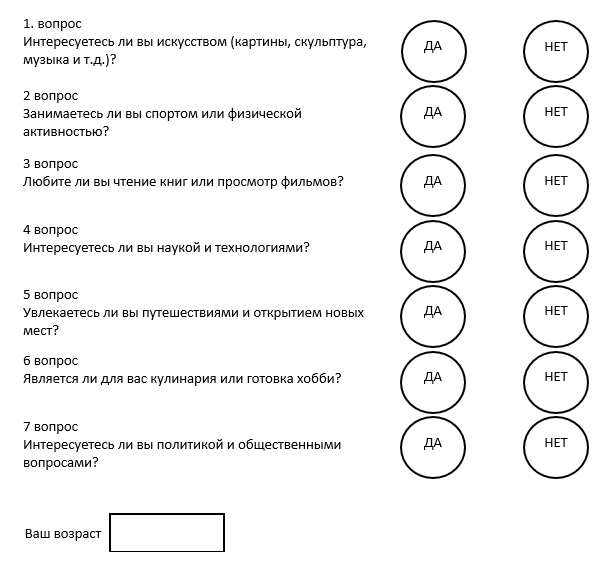
\includegraphics[width=0.7\textwidth]{blank}
% 	\caption{Бланк опроса}
% 	\label{f:blank}
% \end{figure}



% \subsection{Требования к программной документации}

% Состав программной документации должен включать в себя: 

% \begin{itemize}
% 	\item техническое задание; 
% 	\item пояснительная записка, содержащая описание разработки;
% 	\item руководство пользователя.
% \end{itemize}

% Разрабатываемые программные модули должны быть самодокументированы, т.е. тексты программ должны содержать все необходимые комментарии.

% \subsection{Технико-экономические характеристики}

% Реализованное программное обеспечение использует бесплатную модель распространения и разрабатывается с помощью бесплатных решений.


% \section*{Выводы}

% Составлено техническое задание. Были составлены требования к разрабатываемой системе, а также определены основные функции. 



\subsection{Расширенное техническое задание}

Для нагляного отображения доступного пользователю функционала используются диаграмма вариантов использования, которая изображена на рисунке~\ref{f:diag-precedent1}.

\begin{figure}[h!]
    \centering
    \vspace{\toppaddingoffigure}
    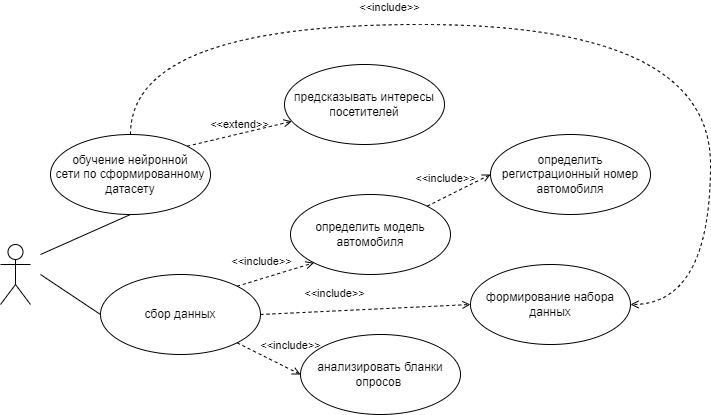
\includegraphics[width=0.7\textwidth]{diag-precedent1}
    \caption{Диаграмма вариантов использования}
    \label{f:diag-precedent1}
\end{figure}

\subsubsection{Основание для разработки}

Программа разрабатывается на основе учебного плана кафедры “Электронные вычислительные машины” по направлению 09.03.01.

\subsubsection{Цель и задача}

Название темы: «Разработка системы оценки и прогнозирования интересов клиентов автостоянки».

Объект - маркетинговое исследование для улучшения качества обслуживания клиентов.

% система оценки и прогнозирования интересов клиентов автостоянки.

Предмет - прогнозирования интересов клиентов автостоянки.

Целью дипломного проекта является помощь маркетологам в понимании предпочтений владельцев автомобилей через автоматизированный сбор и анализ данных, что позволит разрабатывать более точные и персонализированные маркетинговые стратегии. 

Задачи:
\begin{itemize}
    \item автоматизация процесса сбора данных;
    \item распознавание интересов посетителей парковки;
    \item прогнозирование интересов посетителей парковки;
\end{itemize}
% автоматизация процесса сбора данных об интересах посетителей парковки и их прогнозирования.

Результат - разработанная программная система для сбора информации о интересах клиентов и их прогнозироваения. 

\subsubsection{Наименование и область применения}

Наименование разрабатываемого программного обеспечения: система оценки и прогнозирования интересов клиентов автостоянки. 

Область применения: прогнозирование интересов посетителей парковки для улучшения сервиса.


\subsubsection{Требования к функциональности}

Программа должна обеспечивать возможность выполнения следующих функций:

\begin{itemize}
	\item определять регистрационный номер автомобиля;
	\item определять модель автомобиля
	\item анализировать бланки опросов определенного формата;
	\item формирование набора данных в файл типа CSV;
	\item обучение нейронной сети по сформированному датасету;
	\item предсказывать интересы посетителей с использование обученной модели.
\end{itemize}


\subsubsection{Требования к нейронной сети}

Нейронная сеть должна быть реализована на базе языка программирования Python с использованием библиотеки Tensorflow, Keras.


\subsubsection{Требования к бланку}

Бланк должен содержать вопросы и варианты ответа на вопросы (ДА/НЕТ), а также поле для ввода возраста. Пример представлен на рисунке~\ref{f:blank}.

\begin{figure}[ht]
	\centering
	\vspace{\toppaddingoffigure}
	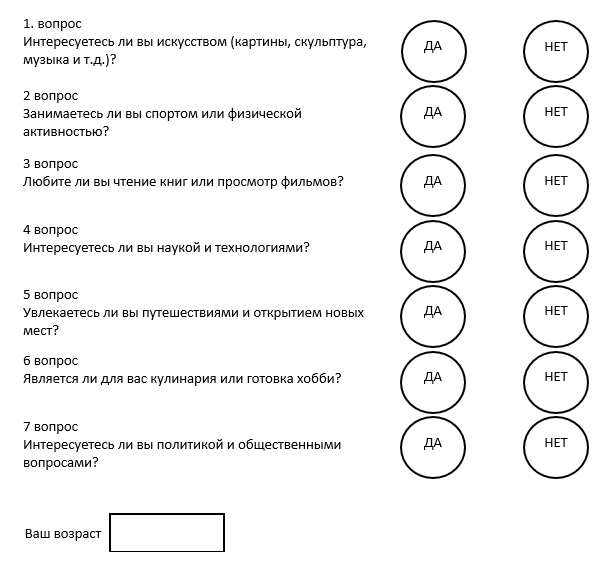
\includegraphics[width=0.7\textwidth]{blank}
	\caption{Бланк опроса}
	\label{f:blank}
\end{figure}



\subsubsection{Требования к программной документации}

Состав программной документации должен включать в себя: 

\begin{itemize}
	\item техническое задание; 
	\item пояснительная записка, содержащая описание разработки;
	\item руководство пользователя.
\end{itemize}

Разрабатываемые программные модули должны быть самодокументированы, т.е. тексты программ должны содержать все необходимые комментарии.

\subsubsection{Технико-экономические характеристики}

Реализованное программное обеспечение использует бесплатную модель распространения и разрабатывается с помощью бесплатных решений.
\newpage

\section{Структура машины времени}

Структура машины времени представлена на рисунке~\ref{f:time-machine}.


\begin{figure}[ht]
	\centering
	\vspace{\toppaddingoffigure}
	
\includegraphics[width=0.7\textwidth]{time-machine}
	\caption{Структура машины времени}
	\label{f:time-machine}
\end{figure}


Разработка структуры машины времени является сложной задачей, поскольку такое устройство находится за пределами существующих научных и инженерных возможностей. Однако, если мы предположим, что машина времени возможна, то ее структура, вероятно, будет иметь следующие основные компоненты:

\begin{enumerate}
	\item часовой механизм: стандартный механизм, который управляет передвижением во времени, аналогично тому, как часовой механизм контролирует передвижение стрелок на циферблате часов;

	\item энергетический источник: мощный источник энергии, способный обеспечить работу машины времени и перемещение объектов во времени;

	\item контрольная система: комплекс алгоритмов и программного обеспечения, которые контролируют точное время и координируют перемещение во времени;

	\item защитные механизмы: системы, предотвращающие нежелательное перемещение во времени или обеспечивающие безопасность при использовании машины времени;

	\item интерфейс пользователя: устройства ввода и вывода, позволяющие пользователю программировать желаемые временные точки или координировать перемещение во времени;

	\item материалы и конструкция: специальные материалы и компоненты, обеспечивающие устойчивость и работоспособность машины времени.
\end{enumerate}

Хотя это очень упрощенное описание возможной структуры машины времени, это может помочь представить основные компоненты, которые потребуются для того, чтобы создать такое устройство. Однако необходимо помнить, что вышеописанная концепция является вымышленной и не имеет научного обоснования.


Пример ссылки на источник \refref{ref:num-methods}.

Пример еще ссылки на источник \refref{ref:time-series-analysis}.

Код представлен в приложении \ref{ax:code}.

Авторская справка представлена в приложении \ref{ax:authornote}.

Какое-то справочное приложение представлено в приложении \ref{ax:ref}.


\subsection{Расчёты}

Расчёты представлены ниже

\begin{gather}
	a = \tan(\frac{\alpha}{2})*a*\pi, \\
	\bigtriangleup b = \cos(\beta)*a, \\
	c = \sin{\beta}.
\end{gather}


\examplecommand

\docappendix{Авторская справка}\label{ax:authornote}
\begin{singlespace}

	\newcommand{\authorfullname}{Жеребцов Кирилл Андреевич}
	\renewcommand{\authorwithinitials}{Жеребцов К. А.}
	\renewcommand{\headofdepartment}{М. Л. Долженкова}

	Я, \authorfullname , автор выпускной квалификационной
	работы «\topic» сообщаю, что мне известно о персональной ответственности автора
	за разглашение сведений, подлежащих защите законами РФ о защите объектов
	интеллектуальной собственности.

	Одновременно сообщаю, что:

	1. При подготовке к защите выпускной квалификационной работы не
	использованы источники (документы, отчёты, диссертации, литература и т.п.),
	имеющие гриф секретности или «Для служебного пользования» ФГБОУ ВО
	«Вятский государственный университет» или другой организации.

	2. Данная работа не связана с незавершёнными исследованиями или уже
	с завершёнными, но ещё официально не разрешёнными к опубликованию
	ФГБОУ ВО «Вятский государственный университет» или другими
	организациями.

	3. Данная работа не содержит коммерческую информацию, способную
	нанести ущерб интеллектуальной собственности ФГБОУ ВО «Вятский
	государственный университет» или другой организации.

	4. Данная работа не является результатом НИР или ОКР, выполняемой по
	договору с организацией.

	5. В предлагаемом к опубликованию тексте нет данных по
	незащищённым объектам интеллектуальной собственности других авторов.

	6. Использование моей дипломной работы в научных исследованиях
	оформляется в соответствии с законодательством РФ о защите интеллектуальной
	собственности отдельным договором.

	\newcommand{\daysize}{2em}

	\newcommand{\confirm}{
		\noindent
		Сведения по авторской справке подтверждаю:~«\uline{\hspace{\daysize}}»
	}

	\newcommand{\verticalspacesize}{2em}

	\newcommand{\rightindent}{2em}

	\newcommand{\customtheyear}{\the\year~г.}

	\newcommand{\rightindentwithyear}{\widthof{\customtheyear}+\rightindent}

	\newcommand{\signaturesize}{6.6em}

	\vspace{\verticalspacesize}


	\noindent
	Автор: \authorwithinitials~«\uline{\hspace{\daysize}}»
	\uline{\hspace{6em}}
	\customtheyear
	\hfill
	\uline{\hspace{\signaturesize}}\hspace{\rightindentwithyear}

	\vspace{-0.3em}
	\hfill
	\makebox[\signaturesize][c]{\small подпись}
	\hspace{\rightindentwithyear}

	\vspace{\verticalspacesize}

	\confirm
	\uline{\hfill}\customtheyear\hspace{\rightindent}

	\vspace{\verticalspacesize}

	\noindent
	Заведующий кафедрой ЭВМ: \headofdepartment
	\hfill
	\uline{\hspace{\signaturesize}}\hspace{\rightindentwithyear}

	\vspace{-0.3em}
	\hfill
	\makebox[\signaturesize][c]{\small подпись}
	\hspace{\rightindentwithyear}

\end{singlespace}




\docappendix{Листинг кода}\label{ax:code}

\begin{lstlisting}
    # Component for searching car models using the autoteka.ru website 
    from selenium import webdriver
    from selenium.webdriver.common.keys import Keys
    from selenium.webdriver.common.by import By
    from selenium.webdriver.support.ui import WebDriverWait  # Импортируем WebDriverWait
    from selenium.webdriver.support import expected_conditions as EC
    import time

    # Path to driver
    driver_path = 'drv/chromedriver-win64/chromedriver.exe'

    # URL link to the page
    website_url = 'https://autoteka.ru/'

    # Initializing the driver
    chrome_service = webdriver.chrome.service.Service(driver_path)
    driver = webdriver.Chrome(service=chrome_service)

    # Function for parsing
    def site(number):
        input = number
        driver.get(website_url)

        input_field = driver.find_element(By.NAME, 'identifier')
        input_field.send_keys(input)
        input_field.send_keys(Keys.ENTER)

        WebDriverWait(driver, 15).until(EC.url_changes(website_url))

        time.sleep(5)

        text_element = driver.find_element(By.CLASS_NAME, 'pit4K')
        text = text_element.text

        time.sleep(3)

        lines = text.split('\n')
        result = ' '.join(lines[:2])

        driver.quit()

        return result.split(',')[0].strip()
\end{lstlisting}

\begin{lstlisting}
    # Component for analyzing forms
    from imutils.perspective import four_point_transform
    from imutils import contours
    import numpy as np
    import argparse
    import imutils
    import cv2
    import csv
    import re
    import pytesseract
    
    # Define the correct answers for the exam (placeholder)
    ANSWER_KEY = {0: 0, 1: 0, 2: 0, 3: 0, 4: 0, 5: 0, 6: 0}
    
    # Path to Tesseract executable
    pytesseract.pytesseract.tesseract_cmd = r'C:\\Program Files\\Tesseract-OCR\\tesseract.exe'
    
    # Tesseract OCR configuration
    custom_config = r'--oem 3 --psm 6'
    
    def process_exam(image_path):
        # Read the input image
        image = cv2.imread(image_path)
        
        # Convert the image to grayscale
        gray = cv2.cvtColor(image, cv2.COLOR_BGR2GRAY)
        
        # Apply GaussianBlur to reduce noise and detail in the image
        blurred = cv2.GaussianBlur(gray, (5, 5), 0)
        
        # Use Canny edge detector to find edges in the image
        edged = cv2.Canny(blurred, 75, 200)
    
        # Find contours in the edged image
        cnts = cv2.findContours(edged.copy(), cv2.RETR_EXTERNAL, cv2.CHAIN_APPROX_SIMPLE)
        cnts = imutils.grab_contours(cnts)
        docCnt = None
    
        # Ensure at least one contour was found
        if len(cnts) > 0:
            # Sort the contours by area, keeping only the largest one
            cnts = sorted(cnts, key=cv2.contourArea, reverse=True)
            for c in cnts:
                # Approximate the contour
                peri = cv2.arcLength(c, True)
                approx = cv2.approxPolyDP(c, 0.02 * peri, True)
                
                # If the approximated contour has four points, assume it's the paper
                if len(approx) == 4:
                    docCnt = approx
                    break
    
        # Apply a perspective transform to obtain a top-down view of the paper
        paper = four_point_transform(image, docCnt.reshape(4, 2))
        warped = four_point_transform(gray, docCnt.reshape(4, 2))
    
        # Apply a binary threshold to the warped image
        thresh = cv2.threshold(warped, 0, 255, cv2.THRESH_BINARY_INV | cv2.THRESH_OTSU)[1]
    
        # Find contours in the thresholded image
        cnts = cv2.findContours(thresh.copy(), cv2.RETR_EXTERNAL, cv2.CHAIN_APPROX_SIMPLE)
        cnts = imutils.grab_contours(cnts)
        questionCnts = []
    
        # Loop over the contours
        for c in cnts:
            (x, y, w, h) = cv2.boundingRect(c)
            ar = w / float(h)
            
            # Filter the contours to find those that correspond to question bubbles
            if (w >= 50) and (h >= 50) and (ar >= 0.9) and (ar <= 1.1):
                questionCnts.append(c)
    
        # Sort the question contours top-to-bottom
        questionCnts = contours.sort_contours(questionCnts, method="top-to-bottom")[0]
        results = []
    
        # Loop over the question groups
        for (q, i) in enumerate(np.arange(0, len(questionCnts), 2)):
            cnts = contours.sort_contours(questionCnts[i:i + 2])[0]
            bubbled = None
            question_result = 0
    
            # Loop over the sorted contours
            for (j, c) in enumerate(cnts):
                mask = np.zeros(thresh.shape, dtype="uint8")
                cv2.drawContours(mask, [c], -1, 255, -1)
    
                mask = cv2.bitwise_and(thresh, thresh, mask=mask)
                total = cv2.countNonZero(mask)
                if bubbled is None or total > bubbled[0]:
                    bubbled = (total, j)
    
            color = (0, 0, 255)
            k = ANSWER_KEY[q]
    
            if k == bubbled[1]:
                question_result = 1
                color = (0, 255, 0)
    
            cv2.drawContours(paper, [cnts[k]], -1, color, 3)
            results.append(question_result)
    
        print(results)
    
        cv2.imshow("Proc", paper)
        cv2.waitKey(0)
    
        return results
    
    def get_age(image_path):
        # Read the input image
        image = cv2.imread(image_path)
        
        # Convert the image to grayscale
        gray = cv2.cvtColor(image, cv2.COLOR_BGR2GRAY)
        
        # Apply GaussianBlur to reduce noise and detail in the image
        blurred = cv2.GaussianBlur(gray, (5, 5), 0)
        
        # Use Canny edge detector to find edges in the image
        edged = cv2.Canny(blurred, 75, 200)
    
        # Find contours in the edged image
        cnts = cv2.findContours(edged.copy(), cv2.RETR_EXTERNAL, cv2.CHAIN_APPROX_SIMPLE)
        cnts = imutils.grab_contours(cnts)
        docCnt = None
    
        # Ensure at least one contour was found
        if len(cnts) > 0:
            # Sort the contours by area, keeping only the largest one
            cnts = sorted(cnts, key=cv2.contourArea, reverse=True)
            for c in cnts:
                # Approximate the contour
                peri = cv2.arcLength(c, True)
                approx = cv2.approxPolyDP(c, 0.02 * peri, True)
                
                # If the approximated contour has four points, assume it's the paper
                if len(approx) == 4:
                    docCnt = approx
                    break
    
        # Apply a perspective transform to obtain a top-down view of the paper
        paper = four_point_transform(image, docCnt.reshape(4, 2))
    
        # Further process the transformed image to find the age
        gray = cv2.cvtColor(paper, cv2.COLOR_BGR2GRAY)
        blurred = cv2.GaussianBlur(gray, (5, 5), 0)
        edged = cv2.Canny(blurred, 75, 200)
    
        cnts = cv2.findContours(edged.copy(), cv2.RETR_EXTERNAL, cv2.CHAIN_APPROX_SIMPLE)
        cnts = imutils.grab_contours(cnts)
        docCnt = None
    
        if len(cnts) > 0:
            cnts = sorted(cnts, key=cv2.contourArea, reverse=True)
            for c in cnts:
                peri = cv2.arcLength(c, True)
                approx = cv2.approxPolyDP(c, 0.02 * peri, True)
                if len(approx) == 4:
                    docCnt = approx
                    break
    
        paper = four_point_transform(paper, docCnt.reshape(4, 2))
    
        gray = cv2.cvtColor(paper, cv2.COLOR_BGR2GRAY)
        thresh = cv2.threshold(gray, 0, 255, cv2.THRESH_BINARY_INV | cv2.THRESH_OTSU)[1]
        
        # Use OCR to extract text from the thresholded image
        text = pytesseract.image_to_string(thresh, config=custom_config)
        
        # Find all two-digit numbers in the extracted text
        number = re.findall(r'\b\d+\b', text)
        two_digit_numbers = ' '.join(num for num in number if len(num) == 2)
        print(two_digit_numbers)
        return two_digit_numbers
    
    def write_to_csv(filename, results):
        # Append the results to a CSV file
        with open(filename, mode='a', newline='') as file:
            writer = csv.writer(file)
            writer.writerow(results)
    
    def blank(path_in, path_out, model):
        print(path_in)
        print(path_out)
        
        # Process the exam and get the age
        results = process_exam(path_in)
        age = get_age(path_in)
        
        # Insert model and age to the results
        results.insert(0, int(age))
        results.insert(0, model)
        
        print(results)
        write_to_csv(path_out, results)
        print("done")
    
    def main():
        # Set up argument parser
        ap = argparse.ArgumentParser()
        ap.add_argument("-i", "--image", required=True, help="path to the input image")
        ap.add_argument("-o", "--output", required=True, help="path to save the output CSV file")
        args = vars(ap.parse_args())
        
        # Process the exam and get the age
        results = process_exam(args["image"])
        age = get_age(args["image"])
        
        # Insert age to the results
        results.insert(0, int(age))
        print(results)
        
        # Write results to the CSV file
        write_to_csv(args["output"], results)
    
    if __name__ == "__main__":
        main()    
\end{lstlisting}

\begin{lstlisting}
    # Component for working with a trained model
    import numpy as np
    import pandas as pd
    import tensorflow as tf
    from sklearn.preprocessing import OneHotEncoder
    import os

    # Transforming new data
    def preprocess_new_data(new_data, full_data):
        # Convert categorical column "Model" to numeric values ​​using OneHotEncoding
        encoder = OneHotEncoder()
        encoder.fit(full_data[['Model']])
        model_encoded = encoder.transform(new_data[['Model']]).toarray()
        
        # Normalization of numerical data (age)
        age = new_data[['Age']].values
        age_normalized = (age - np.mean(full_data['Age'])) / np.std(full_data['Age'])

        # Merging the transformed data
        X_new = np.concatenate([age_normalized, model_encoded], axis=1)
        
        return X_new

    # Receiving Predictions
    def get_predictions(X_new, model_p):
        predictions = model_p.predict(X_new)
        # binary_predictions = np.round(predictions)
        return predictions

    # Output results
    def print_results(binary_predictions):
        # print("New data:")
        # print(new_data)
        print("\nPredictions:")
        np.set_printoptions(threshold=np.inf)
        print(binary_predictions)

    def main(model, age, model_pred):
        
        # Example of new data for testing
        new_data = pd.DataFrame({'Model': [model], 'Age': [int(age)]})

        # Transforming new data
        X_new = preprocess_new_data(new_data, full_data)

        if not os.path.isfile(model_pred):
            raise FileNotFoundError(f"Файл {model_pred} не найден")

        # Check file extension
        if not model_pred.endswith('.keras'):
            raise ValueError("Неправильный формат файла. Ожидался файл с расширением .keras")

        model_p = tf.keras.models.load_model(model_pred)

        # Getting predictions for just one example
        binary_predictions = get_predictions(X_new, model_p)

        art_prediction = binary_predictions[0][0]
        sport_prediction = binary_predictions[0][1]
        book_films_prediction = binary_predictions[0][2]
        science_prediction = binary_predictions[0][3]
        travel_prediction = binary_predictions[0][4]
        cooking_prediction = binary_predictions[0][5]
        politics_prediction = binary_predictions[0][6]

        # Writing to an array
        predictions_array = [art_prediction, sport_prediction, book_films_prediction, science_prediction, travel_prediction, cooking_prediction, politics_prediction]

        return predictions_array
\end{lstlisting}

\begin{lstlisting}
    # Component for training neural networks
    import pandas as pd
    import numpy as np
    import tensorflow as tf
    from tensorflow import keras
    from sklearn.model_selection import train_test_split, GridSearchCV
    from sklearn.preprocessing import OneHotEncoder
    from scikeras.wrappers import KerasClassifier
    from tensorflow.python.keras.callbacks import EarlyStopping, ModelCheckpoint
    from tqdm.keras import TqdmCallback

    # Load the dataset
    data = pd.read_csv('datanew2.csv')

    # Convert the categorical "Model" column to numerical values using OneHotEncoder
    encoder = OneHotEncoder()
    model_encoded = encoder.fit_transform(data[['Model']]).toarray()

    # Normalize the numerical "Age" column
    age = data[['Age']].values
    age_normalized = (age - np.mean(age)) / np.std(age)

    # Combine the normalized age data and the encoded model data
    X = np.concatenate([age_normalized, model_encoded], axis=1)

    # Extract the target variables (interests)
    y = data[['Art', 'Sport', 'Book/Films', 'Science', 'Travel', 'Cooking', 'Politics']].values

    # Split the data into training and test sets
    X_train, X_test, y_train, y_test = train_test_split(X, y, test_size=0.2, random_state=42)

    # Function to create the model with specified parameters
    def create_model(optimizer='adam', num_hidden_layers=2, num_neurons=20, activation='relu', dropout_rate=0.2, learning_rate=0.001):
        # Input layer
        inputs = tf.keras.Input(shape=(X.shape[1],))
        
        # First hidden layer
        x = tf.keras.layers.Dense(num_neurons, activation=activation)(inputs)
        x = tf.keras.layers.Dropout(dropout_rate)(x)
        
        # Additional hidden layers based on the parameter num_hidden_layers
        for _ in range(num_hidden_layers - 1):
            x = tf.keras.layers.Dense(num_neurons, activation=activation)(x)
            x = tf.keras.layers.Dropout(dropout_rate)(x)
        
        # Output layer with sigmoid activation for multi-label classification
        outputs = tf.keras.layers.Dense(7, activation='sigmoid')(x)
        
        # Create the model
        model = tf.keras.Model(inputs=inputs, outputs=outputs)
        
        # Set the optimizer based on the specified parameter
        if optimizer == 'adam':
            optimizer = tf.keras.optimizers.Adam(learning_rate=learning_rate)
        elif optimizer == 'rmsprop':
            optimizer = tf.keras.optimizers.RMSprop(learning_rate=learning_rate)
        elif optimizer == 'sgd':
            optimizer = tf.keras.optimizers.SGD(learning_rate=learning_rate)
        
        # Compile the model
        model.compile(optimizer=optimizer, loss='binary_crossentropy', metrics=['accuracy'])
        return model

    # Create a KerasClassifier with the create_model function
    model = KerasClassifier(model=create_model, verbose=0, epochs=100)

    # Define the grid of parameters for GridSearchCV
    param_grid = {
        'model__num_hidden_layers': [2, 3, 4, 5],
        'model__num_neurons': [20, 30, 40],
        'model__activation': ['relu', 'tanh'],
        'model__dropout_rate': [0.1, 0.2],
        'model__optimizer': ['adam', 'rmsprop', 'sgd'],
        'model__learning_rate': [0.001, 0.01, 0.1]
    }

    # Create a GridSearchCV object
    grid_search = GridSearchCV(estimator=model, param_grid=param_grid, cv=3, verbose=1, n_jobs=-1)

    # Fit the GridSearchCV object to the training data
    grid_search.fit(X_train, y_train)

    # Print the best parameters found by GridSearchCV
    print("Best: %f using %s" % (grid_search.best_score_, grid_search.best_params_))

    # Get the best parameters and create a model with them
    best_params = grid_search.best_params_
    best_model = create_model(
        optimizer=best_params['model__optimizer'],
        num_hidden_layers=best_params['model__num_hidden_layers'],
        num_neurons=best_params['model__num_neurons'],
        activation=best_params['model__activation'],
        dropout_rate=best_params['model__dropout_rate'],
        learning_rate=best_params['model__learning_rate']
    )

    # Define callbacks for early stopping, model checkpointing, and TQDM progress bar
    early_stopping = EarlyStopping(monitor='val_loss', patience=5, restore_best_weights=True)
    model_checkpoint = ModelCheckpoint('model.keras', save_best_only=True, monitor='val_loss', mode='min')
    tqdm_callback = TqdmCallback(verbose=1)

    # Train the best model with the callbacks
    history = best_model.fit(
        X_train, y_train,
        validation_split=0.2,
        epochs=100,
        callbacks=[early_stopping, model_checkpoint, tqdm_callback],
        verbose=0
    )

    # Evaluate the model on the test set
    loss, accuracy = best_model.evaluate(X_test, y_test)
    print(f'Test Accuracy: {accuracy}')
\end{lstlisting}

\begin{lstlisting}
    # Vehicle Number Plate Recognition Component
    import os
    from datetime import timedelta
    from pathlib import Path
    import matplotlib.pyplot as plt
    import cv2
    import numpy as np
    import re
    import imutils
    import pytesseract
    import pytesseract as tess
    tess.pytesseract.tesseract_cmd = r'Tesseract-OCR\tesseract.exe'
    from PyQt6 import uic
    from PyQt6.QtGui import QPixmap
    from PyQt6.QtWidgets import QApplication, QFileDialog, QMessageBox
    from imutils import contours
    from moviepy.editor import VideoFileClip
    import json
    import sqlite3
    import itertools
    import tensorflow as tf
    from skimage.feature import canny
    from skimage.transform import hough_line, hough_line_peaks, rotate
    from skimage.color import rgb2gray

    import matplotlib.gridspec as gridspec
    import cv2

    import autoteka
    import test_blank

    # Constants for saving frames per second from video
    SAVING_FRAMES_PER_SECOND = 1

    # Load the UI design file
    Form, Window = uic.loadUiType("Parking.ui")

    # Initialize the application and load the UI window
    app = QApplication([])
    window = Window()
    form = Form()
    form.setupUi(window)
    window.show()

    # Global variables to store the paths of video, image, and the result
    video_file = ''
    image_file = ''
    result = ''
    arr = []

    # Function to format the time delta for naming frames
    def format_timedelta(td):
        result = str(td)
        try:
            result, ms = result.split(".")
        except ValueError:
            return result + ".00".replace(":", "-")

        ms = round(int(ms) / 10000)
        return f"{result}.{ms:02}".replace(":", "-")

    # Function to load the video file
    def load():
        global video_file
        video_file = QFileDialog.getOpenFileName()
        path = Path(video_file[0])
        video_file = path.name
        print("load")

    # Function to split the video into frames
    def split():
        video_clip = VideoFileClip(video_file)
        filename, _ = os.path.splitext(video_file)

        if not os.path.isdir(filename):
            os.mkdir(filename)

        saving_frames_per_second = min(video_clip.fps, SAVING_FRAMES_PER_SECOND)
        step = 1 / video_clip.fps if saving_frames_per_second == 0 else 1 / saving_frames_per_second

        for current_duration in np.arange(0, video_clip.duration, step):
            frame_duration_formatted = format_timedelta(timedelta(seconds=current_duration)).replace(":", "-")
            frame_filename = os.path.join(filename, f"frame{frame_duration_formatted}.jpg")

            video_clip.save_frame(frame_filename, current_duration)
        print("split")

    # Function to check the format of the recognized license plate
    def check_format(variable):
        pattern = r'^[A-Z]\d{3}[A-Z]{2}\d{3}$'
        pattern2 = r'^[A-Z]\d{3}[A-Z]{2}\d{2}$'
        if re.match(pattern, variable) or re.match(pattern2, variable):
            return True
        else:
            return False

    # Function to choose an image file for recognition
    def choose():
        global image_file
        image_file = QFileDialog.getOpenFileName()
        image_file = image_file[0]
        form.label_6.setPixmap(QPixmap(image_file))
        form.label_6.setScaledContents(True)
        print("choose")

    # Function to recognize text from the car plate
    def carplate_text():
        global image_file

        image0 = cv2.imread(image_file)
        image_height, image_width, _ = image0.shape
        image = cv2.resize(image0, (1024, 1024))
        image = image.astype(np.float32)
        paths = 'model/recognize/model_resnet.tflite'
        interpreter = tf.lite.Interpreter(model_path=paths)
        interpreter.allocate_tensors()
        input_details = interpreter.get_input_details()
        output_details = interpreter.get_output_details()
        X_data1 = np.float32(image.reshape(1, 1024, 1024, 3))

        interpreter.set_tensor(input_details[0]['index'], X_data1)
        interpreter.invoke()
        detection = interpreter.get_tensor(output_details[0]['index'])
        net_out_value2 = interpreter.get_tensor(output_details[1]['index'])
        net_out_value3 = interpreter.get_tensor(output_details[2]['index'])
        net_out_value4 = interpreter.get_tensor(output_details[3]['index'])

        img = image0
        razmer = img.shape

        img2 = cv2.cvtColor(img, cv2.COLOR_BGR2RGB)
        img3 = img[:, :, :]

        number = 0
        while number < len(detection[0][number]) and detection[0, number, 0] > 0.9:
            number = number + 1

        box_x = int(detection[0, number, 0] * image_height)
        box_y = int(detection[0, number, 1] * image_width)
        box_width = int(detection[0, number, 2] * image_height)
        box_height = int(detection[0, number, 3] * image_width)

        cv2.rectangle(img2, (box_y, box_x), (box_height, box_width), (230, 230, 21), thickness=5)

        net_out_value3

        image = image0[box_x:box_width, box_y:box_height, :]
        img2 = cv2.cvtColor(image, cv2.COLOR_BGR2RGB)

        grayscale = rgb2gray(image)
        edges = canny(grayscale, sigma=3.0)
        out, angles, distances = hough_line(edges)
        h, theta, d = out, angles, distances
        angle_step = 0.5 * np.diff(theta).mean()
        d_step = 0.5 * np.diff(d).mean()
        bounds = [np.rad2deg(theta[0] - angle_step),
                np.rad2deg(theta[-1] + angle_step),
                d[-1] + d_step, d[0] - d_step]

        _, angles_peaks, _ = hough_line_peaks(out, angles, distances, num_peaks=20)
        angle = np.mean(np.rad2deg(angles_peaks))

        if 0 <= angle <= 90:
            rot_angle = angle - 90
        elif -45 <= angle < 0:
            rot_angle = angle - 90
        elif -90 <= angle < -45:
            rot_angle = 90 + angle
        if abs(rot_angle) > 20:
            rot_angle = 0

        rotated = rotate(image, rot_angle, resize=True) * 255
        rotated = rotated

        rotated1 = rotated[:, :, :]
        if rotated.shape[1] / rotated.shape[0] < 2:
            minus = np.abs(int(np.sin(np.radians(rot_angle)) * rotated.shape[0]))
            rotated1 = rotated[minus:-minus, :, :]
            print(minus)

        lab = cv2.cvtColor(rotated1, cv2.COLOR_BGR2LAB)
        l, a, b = cv2.split(lab)
        clahe = cv2.createCLAHE(clipLimit=3.0, tileGridSize=(8, 8))
        cl = clahe.apply(l)
        limg = cv2.merge((cl, a, b))
        final = cv2.cvtColor(limg, cv2.COLOR_LAB2BGR)

        letters = ['0', '1', '2', '3', '4', '5', '6', '7', '8', '9', 'A', 'B', 'C', 'E', 'H', 'K', 'M', 'O', 'P', 'T', 'X',
                'Y']

        def decode_batch(out):
            ret = []
            for j in range(out.shape[0]):
                out_best = list(np.argmax(out[j, 2:], 1))
                out_best = [k for k, g in itertools.groupby(out_best)]
                outstr = ''
                for c in out_best:
                    if c < len(letters):
                        outstr += letters[c]
                ret.append(outstr)
            return ret

        paths = 'model/recognize/model1_nomer.tflite'
        interpreter = tf.lite.Interpreter(model_path=paths)
        interpreter.allocate_tensors()

        input_details = interpreter.get_input_details()
        output_details = interpreter.get_output_details()
        img = final
        img = cv2.cvtColor(img, cv2.COLOR_BGR2GRAY)
        img = cv2.resize(img, (128, 64))
        img = img.astype(np.float32)
        img /= 255

        img1 = img.T
        img1.shape
        X_data1 = np.float32(img1.reshape(1, 128, 64, 1))
        input_index = (interpreter.get_input_details()[0]['index'])
        interpreter.set_tensor(input_details[0]['index'], X_data1)

        interpreter.invoke()

        net_out_value = interpreter.get_tensor(output_details[0]['index'])
        pred_texts = decode_batch(net_out_value)
        pred_texts

        fig = plt.figure(figsize=(10, 10))
        outer = gridspec.GridSpec(2, 1, wspace=10, hspace=0.1)
        ax1 = plt.Subplot(fig, outer[0])
        fig.add_subplot(ax1)
        ax2 = plt.Subplot(fig, outer[1])
        fig.add_subplot(ax2)
        return pred_texts[0]

    # Function to recognize the license plate and display information
    def recognize():
        global result
        result = carplate_text().upper()
        print(result)
        if result == '':
            QMessageBox.information(None, "Ошибка распознания", "НЕ РАСПОЗНАНО")
        elif check_format(result) != True:
            QMessageBox.information(None, "Ошибка формата", "Результат:" + result)
        else:
            form.label_7.setText(result)

            count = 0
            for i in range(len(arr)):
                if arr[i][0] == result:
                    count += 1

            if count == 0:
                arr.append([result, 1])
            else:
                for i in range(len(arr)):
                    if arr[i][0] == result:
                        arr[i][1] += 1

            for i in range(len(arr)):
                if arr[i][0] == result:
                    form.label_2.setText(str(arr[i][1]))
                    if arr[i][1] < 5:
                        form.label_5.setText('0%')
                    elif 5 <= arr[i][1] < 10:
                        form.label_5.setText('5%')
                    elif 10 <= arr[i][1] < 20:
                        form.label_5.setText('10%')
                    else:
                        form.label_5.setText('15%')
        
        model = autoteka.site(result)
        print(model)
        print("recognize")

        file_path, _ = QFileDialog.getOpenFileName()
        test_blank.blank(file_path, 'data/data.csv', model)

    # Connect UI buttons to their respective functions
    form.pushButton.clicked.connect(load)
    form.pushButton_2.clicked.connect(split)
    form.pushButton_3.clicked.connect(choose)
    form.pushButton_4.clicked.connect(recognize)

    # Start the application event loop
    app.exec()
\end{lstlisting}

\begin{lstlisting}
    #Interface
    # Importing necessary modules and libraries
    from PyQt6.QtWidgets import (
        QApplication, 
        QWidget, 
        QPushButton, 
        QLabel, 
        QVBoxLayout, 
        QTextEdit, 
        QTableWidget, 
        QTableWidgetItem,
        QTabWidget,
        QMainWindow,
        QFileDialog,
        QMessageBox
    )
    from PyQt6 import QtCore

    # Constant for saving frames per second from a video
    SAVING_FRAMES_PER_SECOND = 1

    # List of interest categories
    list_int = ["Искусство", "Спорт", "Книги/Фильмы", "Наука", "Путешествия", "Кулинария", "Политика"]

    # Global variables for storing file paths and results
    video_file = ''
    image_file = ''
    result = ''
    arr = []

    # Main window class inheriting from QMainWindow
    class MainWindow(QMainWindow):
        def __init__(self):
            super().__init__()

            self.setWindowTitle("Предсказание интересов")
            self.setGeometry(400, 250, 750, 500)

            # Creating a tab widget and setting it as the central widget
            self.tabs = QTabWidget()
            self.setCentralWidget(self.tabs)

            # Creating tabs
            self.create_tabs()

            self.model_pred = ""

        # Method to create tabs
        def create_tabs(self):
            # Creating the first tab for data collection
            tab1 = QWidget()
            
            self.pushButton = QPushButton(tab1)
            self.pushButton.setGeometry(QtCore.QRect(10, 10, 141, 41))
            self.pushButton.setObjectName("pushButton")
            self.pushButton.clicked.connect(self.load)
            self.pushButton.setText("Загрузить видео")

            self.pushButton_2 = QPushButton(tab1)
            self.pushButton_2.setGeometry(QtCore.QRect(10, 60, 141, 41))
            self.pushButton_2.setObjectName("pushButton_2")
            self.pushButton_2.clicked.connect(self.split)
            self.pushButton_2.setText("Разбить на кадры")

            self.pushButton_3 = QPushButton(tab1)
            self.pushButton_3.setGeometry(QtCore.QRect(10, 110, 141, 41))
            self.pushButton_3.setObjectName("pushButton_3")
            self.pushButton_3.clicked.connect(self.choose)
            self.pushButton_3.setText("Выбрать номер")

            self.pushButton_4 = QPushButton(tab1)
            self.pushButton_4.setGeometry(QtCore.QRect(10, 160, 141, 41))
            self.pushButton_4.setObjectName("pushButton_4")
            self.pushButton_4.clicked.connect(self.recognize)
            self.pushButton_4.setText("Распознать номер")

            self.label_6 = QLabel(tab1)
            self.label_6.setGeometry(QtCore.QRect(170, 10, 441, 241))
            self.label_6.setText("")
            self.label_6.setAlignment(QtCore.Qt.AlignmentFlag.AlignCenter)
            self.label_6.setObjectName("label_6")

            self.label_3 = QLabel(tab1)
            self.label_3.setGeometry(QtCore.QRect(200, 340, 71, 21))
            self.label_3.setText("Номер:")
            self.label_3.setObjectName("label_3")

            self.label_7 = QLabel(tab1)
            self.label_7.setGeometry(QtCore.QRect(290, 340, 161, 31))
            self.label_7.setText("")
            self.label_7.setObjectName("label_7")

            # Creating the second tab for neural network training
            tab2 = QWidget()
            tab2_layout = QVBoxLayout()

            self.pushButton_csv = QPushButton(tab2)
            self.pushButton_csv.setText("Выбрать CSV файл")
            self.pushButton_csv.setFixedSize(750, 40)
            self.pushButton_csv.clicked.connect(self.choose_csv_file)
            tab2_layout.addWidget(self.pushButton_csv)

            self.pushButton_learn = QPushButton(tab2)
            self.pushButton_learn.setText("Обучить")
            self.pushButton_learn.setFixedSize(750, 40)
            self.pushButton_learn.clicked.connect(self.learn)
            tab2_layout.addWidget(self.pushButton_learn)

            self.label_csv = QLabel(tab2)
            self.label_csv.setText("CSV файл не выбран")
            tab2_layout.addWidget(self.label_csv)

            tab2.setLayout(tab2_layout)

            # Creating the third tab for prediction
            tab3 = QWidget()
            tab3_layout = QVBoxLayout()

            self.label_model = QLabel('Введите модель', tab3)
            self.label_age = QLabel('Введите возраст', tab3)

            self.text_edit_model = QTextEdit(tab3)
            self.text_edit_model.setFixedSize(750, 30)
            
            self.text_edit_age = QTextEdit(tab3)
            self.text_edit_age.setFixedSize(750, 30)

            self.table = QTableWidget(tab3)
            self.table.setColumnCount(7)
            self.table.setRowCount(2)

            for col in range(7):
                item = QTableWidgetItem(list_int[col])
                self.table.setItem(0, col, item)

            self.button_predict = QPushButton('Получить', tab3)
            self.button_predict.setFixedSize(750, 40)
            self.button_predict.clicked.connect(self.proc)

            self.button_choose_file = QPushButton('Выбрать файл модели', tab3)
            self.button_choose_file.setFixedSize(750, 40)
            self.button_choose_file.clicked.connect(self.choose_model_file)

            # Adding widgets to the third tab
            tab3_layout.addWidget(self.label_model)
            tab3_layout.addWidget(self.text_edit_model)
            tab3_layout.addWidget(self.label_age)
            tab3_layout.addWidget(self.text_edit_age)
            tab3_layout.addWidget(self.button_choose_file)
            tab3_layout.addWidget(self.table)
            tab3_layout.addWidget(self.button_predict)

            tab3.setLayout(tab3_layout)

            # Adding tabs to the QTabWidget
            self.tabs.addTab(tab1, "Сбор данных")
            self.tabs.addTab(tab2, "Обучение нейросети")
            self.tabs.addTab(tab3, "Предсказание")

        # Placeholder method for learning
        def learn(path):
            pass

        # Method to choose a CSV file
        def choose_csv_file(self):
            file_dialog = QFileDialog()
            options = file_dialog.options()
            file_name, _ = QFileDialog.getOpenFileName(self, "Выберите CSV файл", "", "CSV Files (*.csv);;All Files (*)", options=options)
            if file_name:
                self.csv_file = file_name
                self.label_csv.setText(f"Выбранный CSV файл: {file_name}")
            print(self.csv_file)

        # Method to choose a model file
        def choose_model_file(self):
            file_dialog = QFileDialog()
            options = file_dialog.options()
            file_name, _ = QFileDialog.getOpenFileName(self, "Выберите файл модели", "", "Model Files (*.keras);;All Files (*)", options=options)
            if file_name:
                self.model_pred = file_name 
            print(self.model_pred)
            
        # Method to process the model and age input and get predictions
        def proc(self):
            model = self.text_edit_model.toPlainText()
            age = self.text_edit_age.toPlainText()
            if (model != "") & (age != "") & (self.model_pred != ""):
                predictions = test_single.main(model, age, self.model_pred)
                print(predictions)
                for col in range(7):
                    predictions[col] = float(predictions[col])
                    item = QTableWidgetItem(str("{:2.2f}".format(predictions[col] * 100)) + "%")
                    self.table.setItem(1, col, item)

    if __name__ == "__main__":
        app = QApplication(sys.argv)
                
        window = MainWindow()
        window.show()
                
        sys.exit(app.exec()) 
\end{lstlisting}


\docappendix[Справочное]{Библиографический список}

\begin{references}
	\item\label{ref:data-collection} Data Collection [Электронный ресурс] – Режим доступа: https://www.tutorialspoint.com/data-collection, свободный. – Загл. с экрана.

	\item\label{ref:data-analysis} Анализ данных [Электронный ресурс] – Режим доступа: https://en.wikipedia.org/wiki/Data\_analysis, свободный. – Загл. с экрана.

	\item\label{ref:data-visualization} Визуализация данных [Электронный ресурс] – Режим доступа: https://practicum.yandex.ru/blog/vizualizaciya-dannyh/, свободный. – Загл. с экрана.

	\item\label{ref:machine-learning} Машинное обучение: методы и способы [Электронный ресурс] – Режим доступа: https://www.osp.ru/cio/2018/05/13054535, свободный. – Загл. с экрана.

	\item\label{ref:marketing} Медведев П.М. Организация маркетинговой службы с нуля [Текст] ЗАО Издательский дом «Питер». 2005. – 224 с.: ил.

	\item\label{ref:res-net} Exploring ResNet50: An In-Depth Look at the Model Architecture and Code Implementation [Электронный ресурс] – Режим доступа: https://medium.com/@nitishkundu1993/exploring-resnet50-an-in-depth-look-at-the-model-architecture-and-code-implementation-d8d8fa67e46f, свободный. – Загл. с экрана.

	\item\label{ref:cnn-lstm} CNN-LSTM Architecture and Image Captioning [Электронный ресурс] – Режим доступа: https://medium.com/analytics-vidhya/cnn-lstm-architecture-and-image-captioning-2351fc18e8d7, свободный. – Загл. с экрана.
	
	\item\label{ref:neuron} Дюк В.А., Флегонтов А.В., Фомина И.К. Применение технологий интеллектуального анализа данных в естественнонаучных, технических и гуманитарных областях [Текст] Известия Российского государственного педагогического университета им. А.И. Герцена. 2011. No 138.

	\item\label{ref:back-error} Метод обратного распространения ошибки [Электронный ресурс] – Режим доступа: https://education.yandex.ru/handbook/ml/article/metod-obratnogo-rasprostraneniya-oshibki, свободный. – Загл. с экрана.

	\item\label{ref:neuron-model} Neurons in Neural Networks [Электронный ресурс] – Режим доступа: https://www.baeldung.com/cs/neural-networks-neurons, свободный. – Загл. с экрана.

	\item\label{ref:nbc} Наивный байесовский классификатор [Электронный ресурс] – Режим доступа: https://ru.wikipedia.org/wiki/Наивный\_байесовский\_классификатор, свободный. – Загл. с экрана.

	\item\label{ref:log-reg} Пампел Фред, Цвиркун Дмитрий, Груздев Артем. Логистическая регрессия [Текст] ДМК-Пресс, 2023 г. – 218 с.: ил.

	
	\label{ref:total}
\end{references}

\newpage

\docappendix{Библиографический список}

\begin{references}
	\item\label{ref:num-methods} Бахвалов Н.С., Жидков Н.П., Кобельников Г.М.
	Численные методы [Текст] – 4-е изд. – М:. БИНОМ. Лаборатория
	знаний, 2006. – 636 с.: ил.
	\item Безрученко Б.П., Смирнов Д.А.
	Статистическое моделирование по временным рядам [Электронный ресурс]
	Cарат. отд-ние Ин-та радиотехники и электроники РАН.
	– Электрон. дан. – Саратов, 2000. – Режим доступа:
	http://www.masters.donntu.edu.ua/2012/fknt/dorosh/library/article4.pdf,
	свободный. - Загл. с экрана.
	\item Перельмутер А.В. Расчетные модели сооружений и возможность их анализа [Текст] / А.В. Перельмутер, В.И.
	Сливкер. Киев: Сталь, 2002. 600 с.
	\item NeuroShell 2 [Электронный ресурс] – Режим доступа: http://www.neuroproject.ru/aboutproduct.php, свободный. –
	Загл. с экрана.
	\item\label{ref:time-series-analysis} Бокс Дж., Дженкинс Г. Анализ временных рядов.
	Прогноз и управление [Текст]. - М.: Мир, 1974.

	\label{ref:total}
\end{references}


}


\end{document}
